\documentclass[12pt]{article}

% Recommended, but optional, packages for figures and better typesetting:
\usepackage{natbib}
\usepackage{microtype}
\usepackage{subfigure}
\usepackage{booktabs} % for professional tables
\usepackage{fullpage}
\renewcommand{\baselinestretch}{1.2}
% \usepackage{setspace}
% \doublespacing

% hyperref makes hyperlinks in the resulting PDF.
% If your build breaks (sometimes temporarily if a hyperlink spans a page)
% please comment out the following usepackage line and replace
% \usepackage{icml2022} with \usepackage[nohyperref]{icml2022} above.
%\usepackage{hyperref}

\usepackage[breaklinks,colorlinks,
            linkcolor=red,
            anchorcolor=blue,
            citecolor=blue
            ]{hyperref}
% Attempt to make hyperref and algorithmic work together better:
\newcommand{\theHalgorithm}{\arabic{algorithm}}

% For theorems and such
\usepackage{amsmath}
\usepackage{amssymb}
\usepackage{mathtools}
\usepackage{amsthm}
\usepackage{subcaption}
\usepackage{graphicx}
\usepackage{float}
\graphicspath{{Figures/}{../Figures/}{}}

% if you use cleveref..
\usepackage[capitalize,noabbrev]{cleveref}

%%%%%%%%%%%%%%%%%%%%%%%%%%%%%%%%
% THEOREMS
%%%%%%%%%%%%%%%%%%%%%%%%%%%%%%%%
\theoremstyle{plain}
\newtheorem{theorem}{Theorem}[section]
\newtheorem{proposition}[theorem]{Proposition}
\newtheorem{lemma}[theorem]{Lemma}
\newtheorem{corollary}[theorem]{Corollary}
\theoremstyle{definition}
\newtheorem{definition}[theorem]{Definition}
\newtheorem{assumption}[theorem]{Assumption}
\theoremstyle{remark}
\newtheorem{remark}[theorem]{Remark}
\Crefname{assumption}{Assumption}{Assumptions}

\usepackage{relsize}
\usepackage[utf8]{inputenc} % allow utf-8 input
\usepackage[T1]{fontenc}    % use 8-bit T1 fonts
\usepackage{url}            % simple URL typesetting
\usepackage{amsfonts}       % blackboard math symbols
\usepackage{nicefrac}       % compact symbols for 1/2, etc.
\usepackage{smile}
\usepackage{xcolor}
\usepackage{bbm}

\newcommand{\jiyuan}[1]{[\textcolor{green}{Tan: #1}]}
\title{\LARGE Adaptive Estimation and Inference in Conditional Moment Models via the Discrepancy Principle}
\author{Jiyuan Tan\thanks{Jiyuan Tan was supported by NSF Award IIS-2337916.}\and
Vasilis Syrgkanis\thanks{Vasilis Syrgkanis was supported by NSF Award IIS-2337916.}}
\date{}
\begin{document}
\maketitle


\begin{abstract}
We study adaptive estimation and inference in linear inverse problems defined by conditional moment restrictions. Regularization stabilizes such problems, but the regularization parameter depends on a source parameter that is almost never known. We develop a discrepancy principle that chooses this parameter from empirical losses and prescribed bounds on statistical error, without knowing the source parameter. The framework covers Regularized DeepIV (RDIV) and the Tikhonov Regularized Adversarial Estimator (TRAE). Under the stated realizability conditions and comparable fitting and calibration error bounds, both one-step procedures attain strong- and weak-error bounds that match known-source rates for source parameters up to one. We also extend the framework to iterative procedures under realizability of the population iterates, widening the range of source parameters covered by the rate comparison. Finally, we use these adaptive estimators to construct an asymptotically normal doubly robust estimator that adapts to the well-posedness of the primal and dual problems.

\end{abstract}


\section{Introduction}
Ill-posed inverse problems arise throughout causal inference and econometrics \citep{horowitz2014ill}, for example in nonparametric instrumental variable (IV) regression \citep{neweyInstrumentalVariableEstimation2003,darollesNonparametricInstrumentalRegression2011,neweyNonparametricInstrumentalVariables2013,aiEfficientEstimationModels2003}, proximal causal inference \citep{miao2018confounding,tchetgen2020introduction}, and missing-not-at-random problems \citep{d2010new,miao2015identification,breunig2021nonparametric,li2023non}. We study estimating parameters defined by
\[
\theta _{0} =\mathbb{E}\left[\tilde{m}( W;h_{0})\right] ,
\]
where $h\mapsto\tilde m(W;h)$ is a known linear map. The nuisance function $h_0$ solves the conditional moment problem
\begin{equation}\label{eq:cm}
\mathbb{E}[ h_0(X) \mid Z=z] =r_{0}(z) ,
\end{equation}
where $X$ and $Z$ are $W$-measurable random variables. The function $r_0$ represents the expectation of a known linear map: $\mathbb E[m(W;q)]=\mathbb E[r_0(Z)q(Z)]$ for the test functions $q$ that \cref{sec:pre} introduces.

\noindent\textit{Remark (notation).} $r_0\in\tilde{\mathcal Q}$ is the Riesz representer of the continuous linear functional $q\mapsto\mathbb E[m(W;q)]$, satisfying $\mathbb E[m(W;q)]=\mathbb E[r_0(Z)q(Z)]$ for every $q\in\tilde{\mathcal Q}$. In Proposition~\ref{prop:exist_lambda_deepiv}, Theorem~\ref{thm:deepiv_rate}, Proposition~\ref{prop:exist_lambda_iter_rdiv}, Theorem~\ref{thm:iter_rdiv_rate}, Lemma~\ref{lemma:t_err_dp}, Lemma~\ref{lemma:err_l_dp}, Lemma~\ref{lemma:err_r_dp}, Lemma~\ref{lemma:str_dp}, Corollary~\ref{cor:rdiv_discrepancy_bound}, Lemma~\ref{lemma:rdiv_accepted_bounds}, Lemma~\ref{lemma:iter_rdiv_stability}, Corollary~\ref{cor:iter_rdiv_discrepancy_bound}, Lemma~\ref{lemma:iter_rdiv_accepted_bounds}, a result cited in the proof of Lemma~\ref{lemma:err_l_dp}: $\tilde{\mathcal Q}=L_2(Z)$ and $r_0(z)=\mathbb E[Y\mid Z=z]$. The letter $q$ is locally reused for function-valued arguments in $\tilde{\mathcal Q}$ and for a deterministic scalar bias exponent in $(1,\infty)$; these uses denote distinct objects. In Theorem~\ref{thm:common_dp}: In $B_n(\lambda)=C_b\lambda^q$, $q>1$ is a fixed scalar exponent. In Theorem~\ref{thm:deepiv_rate}, Theorem~\ref{thm:tikhonv_rate}: In the application of the generic discrepancy guarantee, the scalar exponent is $q=p=\min\{\beta+1,2\}$. In Theorem~\ref{thm:iter_rdiv_rate}, Theorem~\ref{thm:iter_trae_rate}: In the proof's scalar abbreviation and application of the generic discrepancy guarantee, $q=q_t=\min\{\beta+1,2t\}$. In Corollary~\ref{cor:normality}: In the dual minimization, $q\in\mathcal Q$ is the candidate function of $Z$; in $\hat\theta(h,q)$ it is the dual nuisance argument.


Two established approaches estimate nuisance functions from conditional moment restrictions. Linear inverse problem (LIP) methods formulate the restriction as an operator equation and regularize its solution \citep{carrascoChapter77Linear2007,darollesNonparametricInstrumentalRegression2011,bennett2023source}. Sieve minimum distance methods approximate the unknown functions in finite-dimensional spaces and minimize a sample criterion \citep{aiEfficientEstimationModels2003,chenEstimationNonparametricConditional2012}. We follow the LIP approach. Let $\Pi_{\tilde{\mathcal Q}}$ denote the mean-square projection onto a closed test space. The operator $\mathcal T h=\Pi_{\tilde{\mathcal Q}}\mathbb E[h(X)\mid Z=\cdot]$ then turns \eqref{eq:cm} into the equation $\mathcal T h_0=r_0$. We estimate the minimum-norm solution of this equation with regularized estimators over general hypothesis classes.

While many works use Tikhonov regularization for this inverse problem \citep{neweyNonparametricInstrumentalVariables2013,li2024regularized,bennettInferenceStronglyIdentified2023a,bennett2023source}, a central challenge in applying LIP methods is selecting the regularization parameter. Known-smoothness rate analyses for the Tikhonov regularized adversarial estimator (TRAE) \citep{bennettInferenceStronglyIdentified2023a,bennett2023source} and Regularized DeepIV (RDIV) \citep{li2024regularized} express the regularization level in terms of the source parameter---often encoded by the $\beta$-source condition (i.e., $h_{0}=\left(\mathcal{T}^{*}\mathcal{T}\right)^{\beta/2}w_{0}$ for some $w_{0}\in\tilde{\mathcal{H}}$). \citet{li2024regularized} also study model selection for RDIV. Our procedure selects the regularization level within a fixed hypothesis class. In practice, $\beta$ is rarely known. A misspecified regularization parameter can lead to suboptimal convergence rates or even divergence. The L-curve offers a geometric criterion for choosing the regularization parameter from the solution and residual norms \citep{hansen1992analysis}. Cross-validation (CV) is also widely used, but it requires repeatedly minimizing the loss and is computationally expensive. Moreover, CV typically selects the parameter that minimizes the weak metric; however, this method fails to directly imply a bound in the strong metric. This paper addresses this gap by introducing a discrepancy-principle framework for adaptively selecting a hyperparameter that does not require knowing the exact $\beta$.

\noindent\textit{Remark (notation).} $\beta>0$ is a source exponent satisfying $h_0=(\mathcal T^*\mathcal T)^{\beta/2}w_0$ for some $w_0\in\widetilde{\mathcal H}$. In Corollary~\ref{cor:normality}: The two applications use potentially different source exponents: $h_0=(\mathcal T^*\mathcal T)^{\beta_h/2}w_h$ and $q_0=(\mathcal T\mathcal T^*)^{\beta_q/2}w_q$, with source elements in their respective Hilbert spaces; $\beta_m=\max\{\beta_h,\beta_q\}$. $w_0\in\tilde{\mathcal H}$ is a chosen source witness satisfying $h_0=(\mathcal T^*\mathcal T)^{\beta/2}w_0$, with no uniqueness or unit-norm requirement. In Proposition~\ref{prop:exist_lambda_deepiv}, Proposition~\ref{prop:exist_lambda_iter_rdiv}: When $h_0=0$, take $w_0=0$ in the initial-acceptance argument.


We primarily use the discrepancy principle (DP) \citep{morozov1966solution} from classical inverse problems. DP adaptively selects the regularization parameter $\lambda$ so that the empirical loss is on the same order as the estimated noise level. This data-driven process balances empirical fit and statistical noise. In particular, we extend the classical DP to address the following challenges in our setting. First, classical LIP assumes known operators; in our setting the conditional expectation operator $\mathcal{T}$ is unknown and must be estimated, either explicitly or implicitly, before solving the inverse problem. Second, classical DP assumes fixed, known noise in $r_0$, whereas our noise comes from empirical-process fluctuations and depends on the estimator; see, e.g., the localized concentration bounds in \citet[Lemma~14]{foster2023orthogonal}. Third, classical DP is typically analyzed over full Hilbert spaces with closed-form regularized solutions, while we work with general hypothesis classes (e.g., neural networks) that satisfy inductive-bias assumptions.

\noindent\textit{Remark (notation).} $\lambda$ is the scalar regularization parameter. In the classical Hilbert-space construction \eqref{eq:tikh_sol} and Definition~\ref{def:dp}, finite penalties satisfy $0<\lambda<\infty$, with $\lambda=\infty$ denoting the zero-estimator convention. The value $\lambda=0$ is admitted only for the separate finite-dimensional computational convention of Section~\ref{sec:rkhs_computation}, which selects a minimum-Euclidean-norm solution on the retained spectral subspace; it does not define an unregularized solution of \eqref{eq:tikh_sol} for arbitrary $r_\delta$. In Theorem~\ref{thm:common_dp}, Proposition~\ref{prop:exist_lambda_deepiv}, Theorem~\ref{thm:deepiv_rate}, Proposition~\ref{prop:exist_lambda_iter_rdiv}, Theorem~\ref{thm:iter_rdiv_rate}, Proposition~\ref{prop:exist_lambda}, Theorem~\ref{thm:tikhonv_rate}, Proposition~\ref{prop:exist_lambda_iter_trae}, Theorem~\ref{thm:iter_trae_rate}, Corollary~\ref{cor:normality}: The tuning rule searches the deterministic finite grid $\Lambda_n=\{2\rho^k:k=0,\ldots,K_n\}$, where $1/2\leqslant\rho<1$ and $K_n=\lceil\log(2n^2)/\log(1/\rho)\rceil$; its selected value is denoted $\lambda_{\mathrm{dp}}$. In Proposition~\ref{prop:rkhs_qp}: $\lambda>0$ is a candidate penalty for the unrestricted quadratic program, before the numerical spectral restriction. In Lemma~\ref{eq:iter_trae_strong_propagation}: In each concentration application in the proof, $\lambda\in\Lambda_n\cap[\lambda_{\mathrm{IT}}^\circ,2]$ is a fixed candidate penalty.


In this paper, we propose a discrepancy-principle-based tuning rule without prior information about smoothness. Our main contributions are as follows.
\begin{itemize}
    \item We give a uniform discrepancy rule together with an oracle guarantee that apply to a large class of estimators, and we apply them to RDIV and TRAE. For source parameters up to one, and when fitting and calibration errors are comparable, we show that the discrepancy principle selects a regularization parameter with the same strong- and weak-error rates as in the known-source analysis.
    \item We additionally extend the adaptive estimator to iterated regularized RDIV and TRAE, and we show that, for a prescribed iteration count $t$, the adaptive iterated estimator matches the known-source rates over the range $\beta\leqslant2t-1$.
    \item We combine adaptive TRAE fits of the primal and dual problems into a doubly robust estimator of $\theta_0$. We show that this estimator is asymptotically normal and can adapt to the well-posedness of either problem.
    \item We evaluate the rule with kernel classes in two simulation designs, where the best fixed penalty changes by three orders of magnitude across settings. With a data-driven noise level, the selected penalty follows the best fixed penalty of each setting, and adaptive TRAE has smaller strong, weak, and target errors than any single fixed penalty.
\end{itemize}

\noindent\textit{Remark (notation).} $t\geqslant1$ is a prescribed integer iteration count held fixed as $n$ varies and chosen independently of the data and the source parameter $\beta$.


The rest of the paper proceeds as follows. Section \ref{sec:pre} sets up the problem, fixes notation, and reviews linear inverse problems and the discrepancy principle. Section \ref{sec:dp_regularization} develops the adaptive regularization framework and proves the guarantees for RDIV, TRAE, and doubly robust estimation. Section \ref{sec:experiments} evaluates the rule in simulations with kernel classes, and the conclusion discusses implications and open directions.



\subsection{Related Work}
\paragraph{Nonparametric instrumental variables.}
Nonparametric IV estimation provides a central example of a statistical inverse problem. Sieve and kernel estimators address the ill-posedness of the conditional expectation operator through finite-dimensional approximation or regularization \citep{neweyInstrumentalVariableEstimation2003,hallNonparametricMethodsInference2005,darollesNonparametricInstrumentalRegression2011,chenEstimationNonparametricConditional2012}. The resulting convergence rates depend on both the regularity of the structural function and the operator \citep{chenRATEOPTIMALITYILLPOSED2011,florensIDENTIFICATIONESTIMATIONPENALIZATION2011}. Recent estimators accommodate flexible function classes through kernel methods \citep{singh2019kernel,muandet2020dual}, minimax formulations of the moment restrictions \citep{lewis2018adversarial,dikkala2020minimax,liao2020provably,bennett2023variational}, or two-stage learning of conditional expectations \citep{hartford2017deep,xu2021features,li2024regularized}. Our analysis builds on the regularized least-squares estimator of \citet{li2024regularized} and the regularized adversarial estimator of \citet{bennett2023source}.

\paragraph{Adaptive estimation in IV models.}
Data-driven regularization has an established literature in nonparametric IV models. \citet{johannes2011partially} develop a model-selection procedure that adapts over smoothness classes under restrictions on the conditional expectation operator. \citet{horowitz2014adaptive} select the dimension of a series estimator through an empirical criterion and establish adaptation to unknown smoothness. \citet{breunig2016adaptive} combine model selection and Lepski's method to estimate linear functionals at adaptive rates. More recently, \citet{chen2025adaptive} develop data-driven sieve dimension choices that attain optimal sup-norm rates for structural functions and their derivatives, together with adaptive uniform confidence bands. These procedures adapt the dimension of a sieve or series expansion. We instead fix a general hypothesis class and adapt the Tikhonov penalty itself, combining localized loss bounds for RDIV and TRAE \citep{li2024regularized,bennett2023source} with a discrepancy search over a geometric grid.

\paragraph{Discrepancy principles and iterative regularization.}
The discrepancy principle chooses the amount of regularization by comparing an observed residual with a noise threshold \citep{morozov1966solution,morozov1984methods}. Classical inverse-problem theory relates this rule to source conditions and explains how iterated Tikhonov regularization extends the range of smoothness that the estimator can use \citep{engl1996regularization,nair2003morozov}. Statistical analyses account for the fluctuations of the residual itself. \citet{blanchard2018optimal} establish oracle adaptation in the strong norm for residual stopping rules in linear inverse problems. \citet{celisse2021discrepancy} study discrepancy rules for kernel spectral estimators, including Tikhonov regularization, and derive oracle inequalities and adaptive rates for ordinary and smoothed residuals. \citet{harrach2020beyond} analyze regularization with noise estimated from repeated measurements. Our conditional moment setting adds estimation of the operator and optimization over hypothesis classes. The projected RDIV discrepancy and the adversarial discrepancy account for these statistical errors within a common finite-grid selection argument. The iterative analyses apply this argument to a prescribed number of Tikhonov steps.

\paragraph{Inference on linear functionals.}
Inference on functionals of conditional moment solutions connects this regularization problem to semiparametric estimation \citep{aiEfficientEstimationModels2003}. \citet{bennettInferenceStronglyIdentified2023a} characterize strongly identified linear functionals and construct debiased estimators from regularized primal and dual fits. \citet{bennett2023source} develop source-condition double robustness, under which sufficiently favorable regularity of either inverse problem can support asymptotic normality, and analyze iterated adversarial Tikhonov estimators. We use their primal--dual representation and remainder analysis with discrepancy-selected nuisance estimators. This yields a sufficient condition for asymptotic normality expressed in the primal and dual source parameters while choosing the regularization levels from the data.

\section{Preliminaries}\label{sec:pre}

\textbf{Problem formulation.} We observe independent copies of a random variable $W$ and estimate a linear functional whose nuisance function is defined by a LIP. The target is 
\[
\theta _{0} =\mathbb{E} [\tilde{m} (W;h_{0} )],
\]
with a known linear functional $h\mapsto \tilde{m} (W;h)$. Let $X$ and $Z$ be two $W$-measurable random variables, and let $ \tilde{\mathcal{H}}$ and $ \tilde{\mathcal{Q}}$ be closed linear subspaces of $ L_{2}( X)$ and $ L_{2}( Z)$, respectively, where $L_2(X)$ denotes square-integrable functions of $X$. Let $\mathcal{H} \subset \tilde{\mathcal{H}}$ and $\mathcal{Q} \subset \tilde{\mathcal{Q}}$ be subsets of these function spaces. The classes $\mathcal H$ and $\mathcal Q$ may consist of bounded subsets of reproducing kernel Hilbert spaces, neural networks, or parametric families. We define the linear operator $ \mathcal{T} h=\Pi _{\tilde{\mathcal{Q}}}\mathbb{E}[ h( X) \mid Z=\cdot ]$, where $ \Pi _{\mathcal{V}}$ denotes mean-square projection onto a closed subspace $ \mathcal{V}$. The nuisance function $h_{0}$ is defined as the minimum-norm solution in $\tilde{\mathcal{H}}$ to the LIP
\begin{equation}\label{eq:lin_inv_prob}
\mathcal{T} h_0=r_{0} ,
\end{equation}
where $r_0$ is the Riesz representer of the continuous linear functional $q\mapsto\mathbb E[m(W;q)]$, so that 
\[
\mathbb{E}[ m( W;q)] =\mathbb{E}[ r_0( Z) q( Z)] ,\quad \forall q\in \tilde{\mathcal{Q}} .
\]
We make the following assumption to ensure that solutions exist. 

\noindent\textit{Remark (notation).} $\mathcal H$ denotes the primal hypothesis class of functions of $X$. In Proposition~\ref{prop:rkhs_qp}: $\mathcal H$ is the full RKHS generated by $k_{\mathcal H}$, before restriction to the retained numerical spectral span; its RKHS norm specifies the minimum-norm representative among functions with the same fitting-sample evaluations. $L$ denotes the method-specific population loss functional, defined using population expectations. In Lemma~\ref{lemma:t_err_dp}, Lemma~\ref{lemma:err_l_dp}, Lemma~\ref{lemma:err_r_dp}, a result cited in the proof of Lemma~\ref{lemma:err_l_dp}: $L(h)=\mathbb E[(Y-\mathcal T h(Z))^2]=\sigma^2_{Y\mid Z}+\|\mathcal T(h-h_0)\|^2$, where $\sigma^2_{Y\mid Z}=\mathbb E[(Y-r_0(Z))^2]$. In Proposition~\ref{prop:exist_lambda}, Theorem~\ref{thm:tikhonv_rate}, Proposition~\ref{prop:exist_lambda_iter_trae}, Theorem~\ref{thm:iter_trae_rate}, Corollary~\ref{cor:normality}, Lemma~\ref{lemma:concentrate_l}, Lemma~\ref{lemma:strong_convexity}, Corollary~\ref{cor:trae_discrepancy_bound}, Lemma~\ref{lemma:trae_accepted_bounds}, Lemma~\ref{eq:iter_trae_strong_propagation}, Corollary~\ref{cor:iter_trae_discrepancy_bound}, Lemma~\ref{lemma:iter_trae_accepted_stability}, a result cited in the proof of Lemma~\ref{lemma:concentrate_l}: $L(h)=\sup_{f\in\mathcal F}\mathbb E[2m(W;f)-2h(X)f(Z)-f(Z)^2]$; under the stated closeness assumption, $L(h)=\|\mathcal T(h-h_0)\|^2$ for $h\in\mathcal H$. In a result cited in the proof of Lemma~\ref{lemma:strong_convexity}: $L(h)=\sup_{f\in\mathcal F}\mathbb E[2m(W;f)-2h(X)f(Z)-f(Z)^2]$; under the stated closeness assumption, $L(h)=\|\mathcal T(h-h_0)\|^2$ for $h\in\mathcal H$.


\begin{assumption}\label{asp:range}
We have $ r_{0} \in \mathcal{R}(\mathcal{T}) :=\{\mathcal{T} h:h\in \tilde{\mathcal{H}}\}$.
\end{assumption}
Given an estimated solution $ \hat{h}$ of (\ref{eq:lin_inv_prob}), the strong and weak metrics are defined as 
\[
\| \hat{h} -h_{0} \| _{\text{strong}} =\| \hat{h} -h_{0} \| _{L_{2}} ,\qquad
\| \hat{h} -h_{0} \| _{\text{weak}} =\| \mathcal{T}(\hat{h} -h_{0}) \| _{L_{2}} .
\]
The weak metric measures error only after applying $\mathcal T$, so ill-posedness lets a small weak error coexist with a large strong one. The adjoint of $\mathcal T$ is 
\[
\mathcal T^*q=\Pi_{\tilde{\mathcal H}}\mathbb E[q(Z)\mid X=\cdot] .
\]
Let $a_0$ be the Riesz representer of $h\mapsto\mathbb E[\tilde m(W;h)]$, and let $q_0$ denote the minimum-norm solution, when it exists, of the dual inverse problem
\[
\mathcal{T^{*}} q_{0} =a_{0} .
\]

\noindent\textit{Remark (notation).} The notation $a_0$ is local to either the dual inverse problem or the scalar recursion for $(a_j)_{j\geqslant0}$. In Corollary~\ref{cor:normality}: $a_0\in\tilde{\mathcal H}$ is the Riesz representer satisfying $\mathbb E[\tilde m(W;h)]=\mathbb E[a_0(X)h(X)]$ for every $h\in\tilde{\mathcal H}$, and is the right-hand side of $\mathcal T^*q_0=a_0$. In Lemma~\ref{lemma:iter_rdiv_stability}: In the proof's recursion $a_j=C(1+a_{j-1})$, $a_0=0$ is a scalar initial value, distinct from the Riesz representer in the dual inverse problem.


When the dual problem has a solution, estimates of $h_{0}$ and $q_{0}$ yield the DR estimator \citep{bennett2023source} of $\theta_0$,
\[
\hat{\theta }(\hat{h},\hat{q}) =\mathbb{E}_{n}\left[\tilde{m}( W;\hat{h}) +m( W;\hat{q}) -\hat{q}( Z) \hat{h}( X)\right] .
\]
For \cref{cor:normality}, this empirical average is taken over an evaluation sample independent of the data used to fit and tune the nuisance estimators.


\textbf{Linear inverse problems.} Classical inverse-problem theory studies a noisy observation $r_\delta$ of $r_0$, often with a known operator $\mathcal T$ and error bound $\|r_\delta-r_0\|\leqslant\delta$. Inverting an ill-posed operator can amplify this perturbation. To illustrate this point, suppose that the operator $ \mathcal{T}$ admits a countable singular value decomposition 
\begin{equation}\label{eq:svd}
\mathcal{T} h =\sum _{i=1}^{\infty } \sigma _{i} \langle h,v_{i} \rangle u_{i} ,
\end{equation}
where $\sigma_1\geqslant\sigma_2\geqslant\cdots>0$ are the positive singular values, and $\{v_i\}_{i=1}^{\infty}$ and $\{u_i\}_{i=1}^{\infty}$ form orthonormal bases of $(\ker\mathcal T)^\perp$ and $(\ker\mathcal T^*)^\perp$, respectively. The minimum-norm solution of (\ref{eq:lin_inv_prob}) is
\[
h_{0} =\sum _{i=1}^{\infty }\frac{\langle r_{0} ,u_{i} \rangle }{\sigma _{i}} v_{i} .
\]
The inversion amplifies a perturbation along $u_k$ by $1/\sigma_k$. Tikhonov regularization controls this amplification by solving
\begin{equation}\label{eq:tikh_sol}
h_{\lambda }^{\delta }=\arg\min_{h}\left\{\| \mathcal{T} h-r_{\delta} \| ^{2}+\lambda \| h\| ^{2}\right\}.
\end{equation}
Larger values of $\lambda$ shrink the solution toward zero; smaller values allow greater noise amplification. The discrepancy principle balances these effects through the residual. 
\begin{definition}[Discrepancy Principle]\label{def:dp} Given constants $\ell\in(1,\infty)$ and $\kappa\in(1,\infty)$, choose the regularization parameter $\lambda$ as follows:
\begin{enumerate}
    \item If $ \| r_{\delta } \| \leqslant \kappa \delta $, choose $ h=0$, which corresponds to $ \lambda =\infty $.
    \item If $ \| r_{\delta } \|  >\kappa \delta $, choose $ \lambda $ such that 
    \[
\| \mathcal{T} h_{\lambda }^{\delta } -r_{\delta } \| \leqslant \kappa \delta \leqslant \| \mathcal{T} h_{\lambda '}^{\delta } -r_{\delta } \| ,
\]
    for some $ \lambda '\in [ \lambda ,\ell \lambda ]$.
\end{enumerate}

\noindent\textit{Remark (notation).} $r_\delta\in\tilde{\mathcal Q}$ is a perturbed right-hand side satisfying $\|r_\delta-r_0\|\leqslant\delta$. $\delta\geqslant0$ denotes the prescribed bound in $\|r_\delta-r_0\|\leqslant\delta$ in the classical inverse problem, and the radius of the population-norm restriction $\|f\|\leqslant\delta$ when used as the argument of $\mathfrak R_n(\delta;\mathcal F)$. $h_\lambda^\delta$ is the minimizer over $h\in\tilde{\mathcal H}$ of $\|\mathcal T h-r_\delta\|^2+\lambda\|h\|^2$ for $0<\lambda<\infty$, with $h_\infty^\delta=0$ under the discrepancy rule.


\end{definition}

\noindent\textit{Remark (notation).} $\ell$ takes its meaning from its local binding: a prescribed residual-bracketing factor, an integer iteration index, or a real-valued loss function on $\mathbb R$. In Lemma~\ref{eq:iter_trae_strong_propagation}: In $M_{\leqslant j}=\max_{1\leqslant\ell\leqslant j}\{\lambda,\|f_\ell^*\|_\infty^2\}$ and the subsequent references to $f_\ell^*$, $\ell$ ranges over the integers $1,\ldots,j$. In a result cited in the proof of Lemma~\ref{lemma:strong_convexity}: Put $M=\max\{1,B\}$. Here $\ell:\mathbb R\to\mathbb R$ is the globally Lipschitz loss $\ell(v)=M^2\bigl(\max\{-1,\min\{v,1\}\}\bigr)^2$, with Lipschitz constant $2M^2$; boundedness gives $\ell(h(X)/M)=h(X)^2$ for $h\in\mathcal H$. In Lemma~\ref{lemma:t_err_dp}: In the likelihood concentration argument, $\ell:\mathbb R\to\mathbb R$ is the fixed loss $\ell(v)=-\log\bigl(\max\{1+v,2^{-1/2}\}\bigr)$; it is $\sqrt2$-Lipschitz, satisfies $\ell(0)=0$, and obeys $\ell(f_g-1)=-\log f_g$. In Lemma~\ref{lemma:strong_convexity}: Put $M=\max\{1,B\}$. In the normalized squared-loss argument, $\ell:\mathbb R\to\mathbb R$ is the loss $\ell(u)=M^2\bigl(\max\{-1,\min\{u,1\}\}\bigr)^2$, which is $2M^2$-Lipschitz and satisfies $\ell(h(X)/M)=h(X)^2$ for $h\in\mathcal H$.

The first rule uses the default estimator $h=0$ when the observed right-hand side is no larger than the prescribed noise threshold. The second rule makes the residual $\|\mathcal T h_\lambda^\delta-r_\delta\|$ comparable to that threshold. This residual is measured after applying $\mathcal T$; controlling the reconstruction error in the strong metric additionally requires regularity, such as a source condition. The safety factor $\kappa>1$ makes the second rule feasible: the true solution satisfies $\|\mathcal T h_0-r_\delta\|=\|r_0-r_\delta\|\leqslant\delta<\kappa\delta$, so a residual at the threshold is attainable.

In our statistical setting, both $\mathcal T$ and $r_0$ are unknown, and this ignorance adds perturbations that the classical rule does not face. With an explicit operator estimate $\hat{\mathcal T}_n$, the identity $\hat{\mathcal T}_n h_0=r_0+e_n$, where $e_n=(\hat{\mathcal T}_n-\mathcal T)h_0$, exhibits one such perturbation. Calibration must also absorb empirical fluctuations and, for the raw RDIV squared loss, an irreducible outcome-noise floor. An adversarial estimator never forms $\hat{\mathcal T}_n$ at all, reaching the operator instead through a minimax objective, so its discrepancy carries a different set of errors. One search rule covers both, with a statistical error threshold that may depend on $\lambda$.

To analyze Tikhonov regularization, we introduce the source condition, a standard assumption in the inverse-problem literature. 
\begin{assumption}[Source Condition]\label{asp:source_condition}
Problem (\ref{eq:lin_inv_prob}) satisfies the $ \beta $-source condition for some $ \beta  >0$, i.e., there exists $ w_{0} \in \tilde{\mathcal{H}}$ such that the minimum-norm solution of (\ref{eq:lin_inv_prob}) satisfies $ h_{0} =\left(\mathcal{T}^{*}\mathcal{T}\right)^{\beta /2} w_{0}$.
\end{assumption}

If $\mathcal{T}$ is compact, then by (\ref{eq:svd}), \cref{asp:source_condition} implies that 
$$ \sum_{i=1}^\infty \frac{\langle h_0,v_i \rangle^2}{\sigma^{2\beta}_i} < \infty, $$
which quantifies the decay of the solution coefficients relative to the singular values. This assumption is standard \citep{morozov1966solution,darollesNonparametricInstrumentalRegression2011,li2024regularized,bennettInferenceStronglyIdentified2023a,bennett2023source}.


\textbf{Notation.} Throughout the paper, we use $ \| \cdotp \| $ for the $ L_{2}$ norm with respect to the input distribution, i.e., \[
\| h\| :=\| h\| _{L_{2}} =\sqrt{\mathbb{E}[ h( X)^2]} ,\ \forall h\in L_{2}( X)
\]
and the $L_1$ norm $\|h\|_1=\mathbb E[|h(X)|]$. The same notation applies to functions of $Z$ under their input distribution. Write $\|h\|_{2,n}=\{\mathbb E_n[h(X)^2]\}^{1/2}$ for the empirical norm. For real numbers, $a\vee b=\max\{a,b\}$, and $\log$ denotes the natural logarithm. We use $\mathbb E_n[\cdot]$ to denote an empirical average, with subscripts indicating the sample when several independent samples are used. We use the asymptotic-order notation $o(\cdot)$, $O(\cdot)$, $\Omega(\cdot)$, and $\Theta(\cdot)$; $o_p(1)$ denotes convergence to zero in probability. For a function class $\mathcal F$, let $\operatorname{star}(\mathcal F)=\{\gamma f:\gamma\in[0,1],\ f\in\mathcal F\}$ and $\mathcal F-\mathcal F=\{f-f':f,f'\in\mathcal F\}$. For independent observations $X_1,\ldots,X_n$ from the input distribution, define the expected Rademacher complexity and its localized version by
\begin{align*}
\mathfrak R_n(\mathcal F)&=\mathbb E_{X_{1:n},\epsilon}\left[\sup_{f\in\mathcal F}\left|\frac1n\sum_{i=1}^n\epsilon_i f(X_i)\right|\right],\\
\mathfrak R_n(\delta;\mathcal F)&=\mathbb E_{X_{1:n},\epsilon}\left[\sup_{f\in\mathcal F,\,\|f\|\leqslant\delta}\left|\frac1n\sum_{i=1}^n\epsilon_i f(X_i)\right|\right],
\end{align*}
where the $\epsilon_i$ are independent Rademacher variables, independent of the observations. The localized class uses the population norm. A deterministic critical radius $\delta_{n,\mathcal F}>0$ satisfies
\[
\delta_{n,\mathcal F}^2\geqslant \mathfrak R_n\bigl(\delta_{n,\mathcal F};\operatorname{star}(\mathcal F-\mathcal F)\bigr).
\]
For classes fitted on an independent preliminary sample, we apply this definition conditionally on that sample and use a common deterministic upper bound.

\noindent\textit{Remark (notation).} $\mathcal F$ is a function class on the input domain used in the surrounding complexity or loss definition. In Corollary~\ref{cor:normality}: For the primal application, $\mathcal F\subset\tilde{\mathcal Q}$ is the adversarial test class; for the dual application the corresponding test class is $\mathcal S\subseteq\tilde{\mathcal H}$, with the primal and dual spaces exchanged. In Proposition~\ref{prop:rkhs_qp}: $\mathcal F$ is the full RKHS generated by $k_{\mathcal F}$, and its empirical supremum includes the penalty $-\eta\|f\|_{\mathcal F}^2$ with $\eta>0$. In Proposition~\ref{prop:exist_lambda}, Theorem~\ref{thm:tikhonv_rate}, Proposition~\ref{prop:exist_lambda_iter_trae}, Theorem~\ref{thm:iter_trae_rate}, Lemma~\ref{lemma:concentrate_l}, Lemma~\ref{lemma:strong_convexity}, Corollary~\ref{cor:trae_discrepancy_bound}, Lemma~\ref{lemma:trae_accepted_bounds}, Lemma~\ref{eq:iter_trae_strong_propagation}, Corollary~\ref{cor:iter_trae_discrepancy_bound}, Lemma~\ref{lemma:iter_trae_accepted_stability}, a result cited in the proof of Lemma~\ref{lemma:concentrate_l}, a result cited in the proof of Lemma~\ref{lemma:strong_convexity}: $\mathcal F\subset\tilde{\mathcal Q}$ is the test class in $L_n(h)=\sup_{f\in\mathcal F}\mathbb E_n[2m(W;f)-2h(X)f(Z)-f(Z)^2]$ and its population counterpart; it contains $\mathcal T(h_0-h)$ for every $h\in\mathcal H$ under \cref{asp:closeness}. $\gamma$ is locally bound to its construction, with $\gamma\in[0,1]$ denoting the scalar multiplier in $\operatorname{star}(\mathcal F)=\{\gamma f:\gamma\in[0,1],f\in\mathcal F\}$. In Theorem~\ref{thm:common_dp}: $\gamma\in(0,1]$ is a fixed exponent in the strong-error comparison and the resulting oracle bound. In Theorem~\ref{thm:deepiv_rate}, Theorem~\ref{thm:tikhonv_rate}: When applying the oracle guarantee, the exponent is $\gamma=\min\{\beta,1\}/(1+\min\{\beta,1\})$. In Theorem~\ref{thm:iter_rdiv_rate}, Theorem~\ref{thm:iter_trae_rate}: When applying the oracle guarantee, the exponent is $\gamma=\beta/(\beta+1)$. In Lemma~\ref{lemma:iter_bias}: In the spectral bound, $\gamma>0$ is an arbitrary real exponent in $\sup_{0\leqslant u\leqslant1}u^\gamma\{\lambda/(u+\lambda)\}^{2j}\leqslant C_{\gamma,j}\lambda^{\min\{\gamma,2j\}}$; it is then specialized to $\beta$ and $\beta+1$. In Proposition~\ref{prop:rkhs_qp}: $\gamma\in\mathbb R^N$ is the critic coefficient vector in $f_\gamma(\cdot)=\sum_{j=1}^N\gamma_j k_{\mathcal F}(Z_j,\cdot)$, over which the finite-dimensional critic objective is maximized. $b=\min\{\beta,1\}\in(0,1]$ is the truncated source exponent.

 
\section{Adaptive Regularization via the Discrepancy Principle} \label{sec:dp_regularization}

We now state a finite-grid oracle guarantee for the discrepancy rule applied to estimators of \eqref{eq:lin_inv_prob}, and then check its conditions for two estimators: RDIV, which estimates the operator explicitly, and TRAE, which estimates the weak loss through an adversarial problem.

\subsection{Discrepancy Principle for Conditional Moment Problems}

Consider a family of candidate estimators $\{\hat h_\lambda:\lambda\in\Lambda_n\}$ and a nonnegative calibration statistic $D_n(\hat h_\lambda)$. Fix $\lambda_0=2$ and $\rho\in[1/2,1)$, independent of $n$, and set
\[
K_n=\left\lceil\frac{\log(2n^2)}{\log(1/\rho)}\right\rceil,
\qquad
\Lambda_n=\{\lambda_k=2\rho^k:k=0,\ldots,K_n\}.
\]
Then $|\Lambda_n|=O(\log n)$ and $\lambda_{K_n}\leqslant n^{-2}$. For a prescribed noise level $A_n(\lambda)$, we use the threshold $\tfrac32A_n(\lambda)$. The rule computes the candidates from large to small regularization and returns the first point whose calibration statistic lies below this threshold.

\noindent\textit{Remark (notation).} $\hat h$ denotes an estimated primal solution, with $\hat h_\lambda$ denoting a candidate at penalty $\lambda$, $\hat h_{j,\lambda}$ denoting an empirical iterate, and $\hat h_{\lambda_{\mathrm{dp}}}$ or $\hat h_{t,\lambda_{\mathrm{dp}}}$ denoting the corresponding discrepancy-selected estimate. In Proposition~\ref{prop:exist_lambda_iter_rdiv}, Theorem~\ref{thm:iter_rdiv_rate}, Lemma~\ref{lemma:iter_rdiv_stability}, Corollary~\ref{cor:iter_rdiv_discrepancy_bound}, Lemma~\ref{lemma:iter_rdiv_accepted_bounds}: $\hat h_{0,\lambda}=0$ and $\hat h_{j,\lambda}=\arg\min_{h\in\mathcal H}\{L_n(h)+\lambda\|h-\hat h_{j-1,\lambda}\|_{2,n}^2\}$ for $j=1,\ldots,t$, with the RDIV squared loss; the candidate used for discrepancy selection is $\hat h_{t,\lambda}$. In Corollary~\ref{cor:normality}: $\hat h=\hat h_{\lambda_{\mathrm{dp}}}$ is the one-step adaptive adversarial Tikhonov estimate, with the primal tuning rule run at confidence level $\xi_n/2$ and with the common deterministic sequence $\delta_n$ specified for both nuisance problems. Its evaluations use jointly measurable versions relative to the full nuisance-training and tuning sigma-field $\mathcal G_n$ and the observation, representing the fitted function for almost every training realization and agreeing almost surely with its evaluations at every observation in the finite evaluation sample. In Proposition~\ref{prop:exist_lambda_deepiv}: $\hat h_\lambda=\arg\min_{h\in\mathcal H}\{L_n(h)+\lambda\mathbb E_n[h(X)^2]\}$ with $L_n(h)=\mathbb E_{n,\mathrm{fit}}[(Y-(\hat{\mathcal T}h)(Z))^2]$. In Proposition~\ref{prop:exist_lambda}: $\hat h_\lambda=\arg\min_{h\in\mathcal H}\{L_n(h)+\lambda\mathbb E_n[h(X)^2]\}$, where $L_n(h)=\sup_{f\in\mathcal F}\mathbb E_n[2m(W;f)-2h(X)f(Z)-f(Z)^2]$. In Proposition~\ref{prop:exist_lambda_iter_trae}, Theorem~\ref{thm:iter_trae_rate}, Lemma~\ref{eq:iter_trae_strong_propagation}, Corollary~\ref{cor:iter_trae_discrepancy_bound}, Lemma~\ref{lemma:iter_trae_accepted_stability}: $\hat h_{0,\lambda}=0$ and $\hat h_{j,\lambda}=\arg\min_{h\in\mathcal H}\{L_n(h)+\lambda\|h-\hat h_{j-1,\lambda}\|_{2,n}^2\}$ for $j=1,\ldots,t$, with the adversarial loss; the candidate used for discrepancy selection is $\hat h_{t,\lambda}$. $\hat h_\lambda$ denotes the candidate solution at penalty $\lambda$, with the discrepancy search using the family indexed by $\lambda\in\Lambda_n$ and the candidate construction specified by the estimation method. In Proposition~\ref{prop:exist_lambda}, Theorem~\ref{thm:tikhonv_rate}, Lemma~\ref{lemma:concentrate_l}, Lemma~\ref{lemma:strong_convexity}, Corollary~\ref{cor:trae_discrepancy_bound}, Lemma~\ref{lemma:trae_accepted_bounds}, a result cited in the proof of Lemma~\ref{lemma:concentrate_l}: $\hat h_\lambda$ is a measurable selected minimizer of $L_n(h)+\lambda\mathbb E_n[h(X)^2]$ over $h\in\mathcal H$, where $L_n(h)=\sup_{f\in\mathcal F}\mathbb E_n[2m(W;f)-2h(X)f(Z)-f(Z)^2]$. In Proposition~\ref{prop:exist_lambda_deepiv}, Theorem~\ref{thm:deepiv_rate}, Lemma~\ref{lemma:err_l_dp}, Lemma~\ref{lemma:err_r_dp}, Lemma~\ref{lemma:str_dp}, Corollary~\ref{cor:rdiv_discrepancy_bound}, Lemma~\ref{lemma:rdiv_accepted_bounds}, a result cited in the proof of Lemma~\ref{lemma:err_l_dp}: $\hat h_\lambda$ is a measurable selected minimizer over $h\in\mathcal H$ of $\mathbb E_{n,\mathrm{fit}}[(Y-\hat{\mathcal T}h(Z))^2]+\lambda\mathbb E_{n,\mathrm{fit}}[h(X)^2]$. In Proposition~\ref{prop:exist_lambda_iter_rdiv}, Theorem~\ref{thm:iter_rdiv_rate}, Lemma~\ref{lemma:iter_rdiv_stability}: The candidate supplied to the search is $\hat h_{t,\lambda}$, with $\hat h_{0,\lambda}=0$ and measurable selected minimizers $\hat h_{j,\lambda}\in\arg\min_{h\in\mathcal H}\{L_n(h)+\lambda\|h-\hat h_{j-1,\lambda}\|_{2,n}^2\}$ for $j=1,\ldots,t$, using the RDIV fitting loss. In Corollary~\ref{cor:normality}: The primal candidate is the TRAE measurable selected minimizer of $L_n(h)+\lambda\mathbb E_n[h(X)^2]$ over $\mathcal H$; the corresponding dual construction exchanges the primal and dual spaces and operators. For the selected primal fit $\hat h$, take jointly measurable fitted evaluations representing the fitted function for almost every nuisance-training and tuning realization and agreeing almost surely with $\hat h(X(W_i))$ simultaneously for $i=1,\ldots,n$ in the evaluation sample. In Proposition~\ref{prop:rkhs_qp}: $\widehat h_\lambda$ minimizes $L_{N,\eta}(h)+\lambda\mathbb E_N[h(X)^2]$ over the full RKHS $\mathcal H$, taking the minimum-RKHS-norm representative among functions with the same fitting-sample evaluations; it has the form $\widehat h_\lambda(\cdot)=\sum_{j=1}^N\widehat\alpha_{\lambda,j}k_{\mathcal H}(X_j,\cdot)$ with coefficients solving \eqref{eq:rkhs_qp}. In Proposition~\ref{prop:exist_lambda_iter_trae}, Theorem~\ref{thm:iter_trae_rate}, Lemma~\ref{eq:iter_trae_strong_propagation}, Corollary~\ref{cor:iter_trae_discrepancy_bound}, Lemma~\ref{lemma:iter_trae_accepted_stability}: The candidate supplied to the search is $\hat h_{t,\lambda}$, with $\hat h_{0,\lambda}=0$ and measurable selected minimizers $\hat h_{j,\lambda}\in\arg\min_{h\in\mathcal H}\{L_n(h)+\lambda\|h-\hat h_{j-1,\lambda}\|_{2,n}^2\}$ for $j=1,\ldots,t$, using the TRAE adversarial loss. $D_n$ is the nonnegative discrepancy functional supplied to the search, evaluated at the candidate for each $\lambda\in\Lambda_n$, with its functional definition specified by the estimation method. In Proposition~\ref{prop:exist_lambda_deepiv}, Theorem~\ref{thm:deepiv_rate}, Proposition~\ref{prop:exist_lambda_iter_rdiv}, Theorem~\ref{thm:iter_rdiv_rate}, Lemma~\ref{lemma:err_l_dp}, Corollary~\ref{cor:rdiv_discrepancy_bound}, Lemma~\ref{lemma:rdiv_accepted_bounds}, Lemma~\ref{lemma:iter_rdiv_stability}, Corollary~\ref{cor:iter_rdiv_discrepancy_bound}, Lemma~\ref{lemma:iter_rdiv_accepted_bounds}: $D_n(h)=\mathbb E_{n,\mathrm{cal}}[(\hat r(Z)-\hat{\mathcal T}h(Z))^2]$, the projected calibration residual; the same functional is evaluated at $\hat h_{t,\lambda}$ for iterative candidates. In Corollary~\ref{cor:normality}: For each nuisance problem, the discrepancy is its empirical adversarial loss: $D_n=L_n$ for the primal problem, with the corresponding loss after exchanging the primal and dual spaces and operators for the dual problem. In Proposition~\ref{prop:exist_lambda}, Theorem~\ref{thm:tikhonv_rate}, Proposition~\ref{prop:exist_lambda_iter_trae}, Theorem~\ref{thm:iter_trae_rate}, Lemma~\ref{lemma:trae_accepted_bounds}, Corollary~\ref{cor:iter_trae_discrepancy_bound}, Lemma~\ref{lemma:iter_trae_accepted_stability}, a result cited in the proof of Lemma~\ref{lemma:concentrate_l}: $D_n(h)=L_n(h)=\sup_{f\in\mathcal F}\mathbb E_n[2m(W;f)-2h(X)f(Z)-f(Z)^2]$, with the same loss evaluated at the final iterate for iterative candidates. $A_n:\Lambda_n\to[0,\infty)$ supplies the noise level in the acceptance threshold $\tfrac32A_n(\lambda)$, with prescribed statistical-error bounds in the theoretical constructions and data-dependent noise-floor estimates in the experimental construction. In Theorem~\ref{thm:common_dp}: $A_n$ is prescribed, and is required to be nonincreasing only over $\Lambda_n\cap[\lambda^\circ,2]$. In Proposition~\ref{prop:exist_lambda_deepiv}, Theorem~\ref{thm:deepiv_rate}: $A_n=A_n^{\mathrm R}$, where $A_n^{\mathrm R}(\lambda)=\delta_n^2/\lambda+\nu_n^2$ for $\lambda\in\Lambda_n$. In Proposition~\ref{prop:exist_lambda_iter_rdiv}, Theorem~\ref{thm:iter_rdiv_rate}: $A_n=A_{n,t}^{\mathrm R}$, where $A_{n,t}^{\mathrm R}(\lambda)=s_{n,t}^{\mathrm R}/\lambda+\nu_n^2$ and $s_{n,t}^{\mathrm R}=a_t\delta_n^2$. In Proposition~\ref{prop:exist_lambda}, Theorem~\ref{thm:tikhonv_rate}, Corollary~\ref{cor:normality}: $A_n=A_n^{\mathrm T}$, where $A_n^{\mathrm T}(\lambda)=\delta_n^2$ for $\lambda\in\Lambda_n$, using the TRAE accuracy scale for the relevant problem. In Proposition~\ref{prop:exist_lambda_iter_trae}, Theorem~\ref{thm:iter_trae_rate}: $A_n=A_{n,t}^{\mathrm T}$, where $A_{n,t}^{\mathrm T}(\lambda)=\delta_n^2+\min\{\lambda,s_{n,t}^{\mathrm T}/\lambda\}$ and $s_{n,t}^{\mathrm T}=b_t\delta_n^2$; on the oracle segment $[\lambda_{\mathrm{IT}}^\circ,2]$ this equals $\delta_n^2+s_{n,t}^{\mathrm T}/\lambda$.


\begin{algorithm}[H]
    \caption{Adaptive Regularization via Discrepancy Principle}
    \label{alg:discrepancy}
    \begin{algorithmic}[1]
        \STATE \textbf{Input:} Candidate estimators $\hat h_\lambda$, discrepancy $D_n$, noise level $A_n$.
        \STATE \textbf{Input:} Initial parameter $\lambda_0=2$, search factor $1/2\leqslant\rho<1$.
        \STATE Set $K_n=\lceil\log(2n^2)/\log(1/\rho)\rceil$.
        \FOR{$k=0,\ldots,K_n$}
            \STATE Set $\lambda=\lambda_0\rho^k$ and compute $\hat h_\lambda$.
            \STATE Evaluate $D_n(\hat h_\lambda)$.
            \IF{$D_n(\hat h_\lambda)\leqslant\tfrac32 A_n(\lambda)$}
                \STATE \textbf{Output:} $\lambda$ and $\hat h_\lambda$; terminate.
            \ENDIF
        \ENDFOR
        \STATE \textbf{Output:} $\lambda_{K_n}$ and $\hat h_{\lambda_{K_n}}$ (fallback, used only if no candidate clears its threshold).
    \end{algorithmic}
\end{algorithm}

\noindent\textit{Remark (notation).} In the discrepancy grid, $\rho\in[1/2,1)$ is the fixed search factor, independent of $n$; the notation $\rho$ in the experimental designs of Section~\ref{sec:experiments} instead denotes their instrument-strength parameter, equal to the correlation of $(X,Z)$ in the linear Gaussian design.


If no candidate clears its threshold, the rule returns the terminal point $\lambda_{K_n}$, so the selected estimator is defined for every outcome. \Cref{thm:common_dp} and \cref{prop:exist_lambda_deepiv,prop:exist_lambda} show that the rule accepts a candidate, and so never reaches the fallback, on the events they describe.

When the rule accepts a noninitial parameter, the selected point $\lambda_{\mathrm{dp}}$ and its rejected predecessor $\lambda'=\lambda_{\mathrm{dp}}/\rho\in[\lambda_{\mathrm{dp}},2\lambda_{\mathrm{dp}}]$ satisfy
\begin{equation}\label{eq:discrepancy_principle}
D_n(\hat h_{\lambda_{\mathrm{dp}}})\leqslant\tfrac32A_n(\lambda_{\mathrm{dp}}),
\qquad
D_n(\hat h_{\lambda'})>\tfrac32A_n(\lambda').
\end{equation}
Acceptance at $\lambda_{\mathrm{dp}}$ bounds the weak error; rejection at $\lambda'$, or acceptance at an oracle point, keeps $\lambda_{\mathrm{dp}}$ from falling too far.

\noindent\textit{Remark (notation).} $\lambda_{\mathrm{dp}}=2\rho^{k_*}$, where $k_*=\min\{k\in\{0,\ldots,K_n\}:D_n(\hat h_{2\rho^k})\leqslant\tfrac32A_n(2\rho^k)\}$ if this set is nonempty, and $k_*=K_n$ otherwise, using the candidates, discrepancy, and noise level supplied to the rule. In Proposition~\ref{prop:exist_lambda_deepiv}, Theorem~\ref{thm:deepiv_rate}: The rule uses the one-step RDIV candidates $\hat h_\lambda$, the projected calibration discrepancy, and $A_n^{\mathrm R}(\lambda)=\delta_n^2/\lambda+\nu_n^2$. In Proposition~\ref{prop:exist_lambda}, Theorem~\ref{thm:tikhonv_rate}: The rule uses the one-step TRAE candidates, $D_n=L_n$, and $A_n^{\mathrm T}(\lambda)=\delta_n^2$. In Corollary~\ref{cor:normality}: The primal and dual TRAE problems are tuned separately at confidence levels $\xi_n/2$ using a common deterministic accuracy bound $\delta_n$; the dual output is $\lambda_{\mathrm{dp}}^{\text{dual}}$. In Proposition~\ref{prop:exist_lambda_iter_rdiv}: The rule uses the terminal iterative RDIV candidates $\hat h_{t,\lambda}$, the projected calibration discrepancy, and $A_{n,t}^{\mathrm R}(\lambda)=s_{n,t}^{\mathrm R}/\lambda+\nu_n^2$; its selected parameter is denoted $\lambda_{\mathrm{dp},t}^{\mathrm R}$. In Proposition~\ref{prop:exist_lambda_iter_trae}: The rule uses the terminal iterative TRAE candidates and $A_{n,t}^{\mathrm T}(\lambda)=\delta_n^2+\min\{\lambda,s_{n,t}^{\mathrm T}/\lambda\}$.


The statistic $D_n(\hat h_\lambda)$ plays the role of the squared residual in \cref{def:dp}, and $\tfrac32A_n(\lambda)$ plays the role of $\kappa^2\delta^2$. For RDIV, $D_n$ is a squared residual computed from estimates of the operator and right-hand side. For TRAE, it is an empirical adversarial loss. The statistical bounds in \eqref{eq:common_accepted_bounds} turn a small discrepancy into a small squared weak error. When the first accepted parameter has a predecessor, the two inequalities in \eqref{eq:discrepancy_principle} bracket the threshold at adjacent grid points with ratio $1/\rho\in(1,2]$.

The following theorem states conditions on the discrepancy bound and threshold under which the rule has an oracle guarantee. Throughout, $\xi\in(0,1)$ is a generic confidence level; we absorb fixed numerical rescalings of $\xi$ into the rate bounds and relabel it after intersecting finitely many event families.

\noindent\textit{Remark (notation).} $\xi\in(0,1)$ is a prescribed failure-probability level, with fixed numerical rescalings absorbed into the rate bounds and the level relabelled after intersecting finitely many event families. In Corollary~\ref{cor:normality}: The confidence level used in each primal and dual tuning rule is $\xi_n/2$, where $\xi_n\downarrow0$ is deterministic; the simultaneous nuisance bounds consequently have failure probability at most $\xi_n$.


\begin{theorem}[Oracle guarantee for the discrepancy rule]\label{thm:common_dp}
Let $A_n:\Lambda_n\to[0,\infty)$, and let $\mathcal S_n\subseteq(0,2]$ be a stability region. Fix constants $C_A,C_V,C_b>0$ and exponents $\gamma\in(0,1]$ and $q>1$, and write $B_n(\lambda)=C_b\lambda^q$. Suppose that, on an event $\mathcal E_n$ with probability at least $1-\xi$, the discrepancy bound
\begin{equation}\label{eq:common_discrepancy_bound}
D_n(\hat h_\lambda)\leqslant A_n(\lambda)+B_n(\lambda),
\end{equation}
  holds simultaneously over $\lambda\in\Lambda_n\cap\mathcal S_n$, and every $\lambda\in\Lambda_n\cap\mathcal S_n$ satisfies
\begin{equation}\label{eq:common_accepted_bounds}
\begin{aligned}
\|\mathcal T(\hat h_\lambda-h_0)\|^2
&\leqslant C_A\{D_n(\hat h_\lambda)+A_n(\lambda)\},\\
\|\hat h_\lambda-h_0\|^2
&\leqslant C_V\left[\frac{D_n(\hat h_\lambda)+A_n(\lambda)}{\lambda}+\{D_n(\hat h_\lambda)+A_n(\lambda)\}^\gamma\right],
\end{aligned}
\end{equation}
Suppose that some grid point $\lambda^\circ$ satisfies $\Lambda_n\cap[\lambda^\circ,2]\subseteq\mathcal S_n$, that $A_n$ is nonincreasing over the grid points in $[\lambda^\circ,2]$, and that
\begin{equation}\label{eq:common_oracle_crossing}
B_n(\lambda^\circ)\leqslant\tfrac12A_n(\lambda^\circ).
\end{equation}
Then \cref{alg:discrepancy} accepts a candidate before exhausting the grid, and returns a parameter satisfying $\lambda_{\mathrm{dp}}\geqslant\lambda^\circ$ with
\begin{align}\label{eq:common_rate}
\|\mathcal T(\hat h_{\lambda_{\mathrm{dp}}}-h_0)\|^2
&\leqslant O\{A_n(\lambda^\circ)\},\\
\|\hat h_{\lambda_{\mathrm{dp}}}-h_0\|^2
&\leqslant O\{A_n(\lambda^\circ)/\lambda^\circ+A_n(\lambda^\circ)^\gamma\}.
\end{align}
\end{theorem}

\noindent\textit{Remark.} On $\mathcal E_n$, the algorithm terminates through its acceptance branch at an index $k\leqslant k^\circ$, where $\lambda^\circ=2\rho^{k^\circ}$ and $k^\circ\leqslant K_n$; acceptance at $k=K_n$ is allowed, and both error bounds hold on this event.

\noindent\textit{Remark (notation).} $\mathcal S$ is a fixed population function class whose local definition specifies its role and whether its functions have argument $X$ or $(X,Z)$. In Corollary~\ref{cor:normality}: $\mathcal S$ is the dual test class appearing in $L_n^{\mathrm{dual}}(q)=\sup_{s\in\mathcal S}\mathbb E_n[2\tilde m(W;s)-2q(Z)s(X)-s(X)^2]$. In Lemma~\ref{lemma:strong_convexity}, a result cited in the proof of Lemma~\ref{lemma:strong_convexity}: $\mathcal S=\operatorname{star}(\mathcal H-\mathcal H)$ is the star-shaped difference class used to verify the anchored critical-radius condition. In Lemma~\ref{lemma:t_err_dp}: In the likelihood concentration argument, $\mathcal S=\operatorname{star}(\mathcal G_0-\mathcal G_0)$ is the fixed star-shaped difference class of likelihood-transform functions on $(X,Z)$, with norm $\|\cdot\|_{L_2(X,Z)}$. $\mathcal S_n\subseteq(0,2]$ is the prescribed stability domain for the generic comparisons, which are required at grid points in $\Lambda_n\cap\mathcal S_n$. In Theorem~\ref{thm:deepiv_rate}, Theorem~\ref{thm:tikhonv_rate}: $\mathcal S_n=(0,2]$. In Theorem~\ref{thm:iter_rdiv_rate}: $\mathcal S_n=[\lambda_{\mathrm{IR}}^\circ,2]$ in the application of the generic comparison argument. In Theorem~\ref{thm:iter_trae_rate}: $\mathcal S_n=[\lambda_{\mathrm{IT}}^\circ,2]$ in the application of the generic comparison argument. $\mathcal E_n$ is a common event of probability at least $1-\xi$ on which the relevant comparisons hold simultaneously over their stated function and grid domains. In Proposition~\ref{prop:exist_lambda}, Theorem~\ref{thm:tikhonv_rate}, Lemma~\ref{lemma:concentrate_l}, Lemma~\ref{lemma:strong_convexity}, Corollary~\ref{cor:trae_discrepancy_bound}, Lemma~\ref{lemma:trae_accepted_bounds}: $\mathcal E_n$ is the common TRAE concentration event formed using $\eta_n=\xi/(K_n+1)$ and a union bound over $\Lambda_n$; it includes the uniform loss comparison, the localized squared-norm comparison, and $L_n(h_0)\leqslant C\delta_n^2$. $\lambda^\circ\in\Lambda_n$ is any oracle comparison point satisfying $\Lambda_n\cap[\lambda^\circ,2]\subseteq\mathcal S_n$, nonincreasing $A_n$ on that grid segment, and $B_n(\lambda^\circ)\leqslant\tfrac12A_n(\lambda^\circ)$; no uniqueness or computable selection rule is required. $B$ is a fixed finite nonnegative uniform envelope bound for the quantities specified in the applicable boundedness assumptions. In Proposition~\ref{prop:exist_lambda}, Theorem~\ref{thm:tikhonv_rate}, Proposition~\ref{prop:exist_lambda_iter_trae}, Theorem~\ref{thm:iter_trae_rate}, Corollary~\ref{cor:normality}, Lemma~\ref{lemma:concentrate_l}, Lemma~\ref{lemma:strong_convexity}, Corollary~\ref{cor:trae_discrepancy_bound}, Lemma~\ref{lemma:trae_accepted_bounds}, Lemma~\ref{eq:iter_trae_strong_propagation}, Corollary~\ref{cor:iter_trae_discrepancy_bound}, Lemma~\ref{lemma:iter_trae_accepted_stability}, a result cited in the proof of Lemma~\ref{lemma:concentrate_l}, a result cited in the proof of Lemma~\ref{lemma:strong_convexity}: $|m(W;f)|$, $|h(X)|$, and $|f(Z)|$ are almost surely bounded by $B$, uniformly over $h\in\mathcal H$ and $f\in\mathcal F$; for a dual fit the corresponding bound uses the exchanged primal and dual objects. In Proposition~\ref{prop:exist_lambda_deepiv}, Theorem~\ref{thm:deepiv_rate}, Proposition~\ref{prop:exist_lambda_iter_rdiv}, Theorem~\ref{thm:iter_rdiv_rate}, Lemma~\ref{lemma:t_err_dp}, Lemma~\ref{lemma:err_l_dp}, Corollary~\ref{cor:rdiv_discrepancy_bound}, Lemma~\ref{lemma:rdiv_accepted_bounds}, Lemma~\ref{lemma:iter_rdiv_stability}, Corollary~\ref{cor:iter_rdiv_discrepancy_bound}, Lemma~\ref{lemma:iter_rdiv_accepted_bounds}, a result cited in the proof of Lemma~\ref{lemma:err_l_dp}: $|Y|\leqslant B$ almost surely, $|h(x)|\leqslant B$ for every $h\in\mathcal H$ on the common support of the conditional densities, and $|\hat r(z)|\leqslant B$.


The rule uses the statistical-error bound $A_n$ without evaluating the unknown bias bound $B_n$. It compares $D_n$ with $\tfrac32A_n$. Condition \eqref{eq:common_oracle_crossing} guarantees that such a point exists, so the rule accepts $\lambda^\circ$ whenever it reaches it; because the search runs from large to small regularization, it stops at some $\lambda_{\mathrm{dp}}\geqslant\lambda^\circ$. Acceptance at $\lambda_{\mathrm{dp}}$ caps the discrepancy there by $\tfrac32A_n(\lambda_{\mathrm{dp}})$, and monotonicity carries $A_n(\lambda)$ and $A_n(\lambda)/\lambda$ back to $\lambda^\circ$, which gives \eqref{eq:common_rate}.

We will specify $D_n$, $A_n$, and $\mathcal S_n$ for RDIV and TRAE in the following subsections, writing $V_n$ there for the method-specific component of $A_n(\lambda)/\lambda$. The proof is in \cref{sec:proof_common_dp}.

\paragraph{Noise calibration.}
The tuning rule takes valid statistical-error bounds as inputs. In the following analyses, $\delta_n$ and $\nu_n$ denote deterministic upper bounds multiplied by fixed constants large enough to absorb the concentration and stability constants. These multipliers may depend on the boundedness, density-ratio, and mean-square-continuity constants, but are independent of $n$, $\lambda$, and the unknown source parameter. They are fixed before fitting the candidate estimators. The constants $a_t$ and $b_t$ used for the iterative procedures also absorb the propagation constants for the prescribed iteration count. The discrepancy bounds in the Appendix show that such choices exist. This convention establishes adaptation to the source parameter conditional on valid bounds for the function classes and preliminary nuisances. Estimating all of these bounds from the data requires a separate calibration analysis.

\noindent\textit{Remark (notation).} $\delta_n$ is a prescribed deterministic, method-specific statistical-error bound varying with $n$, calibrated before fitting by fixed multipliers independent of $n$, $\lambda$, and the unknown source parameter. In Proposition~\ref{prop:exist_lambda_iter_rdiv}, Theorem~\ref{thm:iter_rdiv_rate}, Lemma~\ref{lemma:iter_rdiv_stability}, Corollary~\ref{cor:iter_rdiv_discrepancy_bound}, Lemma~\ref{lemma:iter_rdiv_accepted_bounds}: The iteration--grid confidence allocation is $\eta_{n,t}=\xi/\{t(K_n+1)\}$; the resulting $\log t$ contribution is absorbed into a constant adjustment of $\delta_n$ for fixed $t$. In Proposition~\ref{prop:exist_lambda}, Theorem~\ref{thm:tikhonv_rate}, Lemma~\ref{lemma:concentrate_l}, Lemma~\ref{lemma:strong_convexity}, Corollary~\ref{cor:trae_discrepancy_bound}, Lemma~\ref{lemma:trae_accepted_bounds}, a result cited in the proof of Lemma~\ref{lemma:concentrate_l}, a result cited in the proof of Lemma~\ref{lemma:strong_convexity}: $\delta_n$ is the TRAE scale, unrelated to the RDIV scales, satisfying $\delta_n\geqslant\max\{\tilde\delta_n(\eta_n),n^{-1/2}\}$ and $\delta_n=o(1)$, with $\eta_n=\xi/(K_n+1)$. In Corollary~\ref{cor:normality}: $\delta_n$ is a common deterministic TRAE bound for both primal and dual problems, each tuned at confidence level $\xi_n/2$ for a deterministic $\xi_n\downarrow0$, and additionally satisfies $\delta_n=o(n^{-\alpha_{\mathrm{dr}}})$, where $\alpha_{\mathrm{dr}}=(1+\min\{\beta_m,1\})/(2+4\min\{\beta_m,1\})$ and $\beta_m=\max\{\beta_h,\beta_q\}$. In Proposition~\ref{prop:exist_lambda_iter_trae}, Theorem~\ref{thm:iter_trae_rate}, Lemma~\ref{eq:iter_trae_strong_propagation}, Corollary~\ref{cor:iter_trae_discrepancy_bound}, Lemma~\ref{lemma:iter_trae_accepted_stability}: $\delta_n$ is the TRAE scale satisfying $\delta_n\geqslant\max\{\tilde\delta_n(\eta_{n,t}),n^{-1/2}\}$ and $\delta_n=o(1)$, with $\eta_{n,t}=\xi/\{t(K_n+1)\}$. In Proposition~\ref{prop:exist_lambda_deepiv}, Theorem~\ref{thm:deepiv_rate}, Proposition~\ref{prop:exist_lambda_iter_rdiv}, Theorem~\ref{thm:iter_rdiv_rate}, Lemma~\ref{lemma:t_err_dp}, Lemma~\ref{lemma:err_l_dp}, Lemma~\ref{lemma:err_r_dp}, Lemma~\ref{lemma:str_dp}, Corollary~\ref{cor:rdiv_discrepancy_bound}, Lemma~\ref{lemma:rdiv_accepted_bounds}, Lemma~\ref{lemma:iter_rdiv_stability}, Corollary~\ref{cor:iter_rdiv_discrepancy_bound}, Lemma~\ref{lemma:iter_rdiv_accepted_bounds}, a result cited in the proof of Lemma~\ref{lemma:err_l_dp}: $\delta_n$ is the RDIV fitting scale satisfying $\delta_n\geqslant\delta_{n,\mathcal G}+\delta_{n,\mathcal H}+\delta_{n,\xi}$ and $\delta_n+\nu_n=o(1)$. $\nu_n$ is a prescribed deterministic RDIV projected-discrepancy accuracy bound, fixed before fitting the candidates, with $\nu_n\geqslant\delta_{n,\mathcal G}+\delta_{n,r}+\delta_{n,\xi}$ and $\delta_n+\nu_n=o(1)$; its calibration multipliers are independent of $n$, $\lambda$, and the unknown source parameter. In Proposition~\ref{prop:exist_lambda_iter_rdiv}, Theorem~\ref{thm:iter_rdiv_rate}, Lemma~\ref{lemma:iter_rdiv_stability}, Corollary~\ref{cor:iter_rdiv_discrepancy_bound}, Lemma~\ref{lemma:iter_rdiv_accepted_bounds}: The bounds use the iteration--grid confidence allocation $\eta_{n,t}=\xi/\{t(K_n+1)\}$; the resulting $\log t$ contribution is absorbed into a constant adjustment of $\nu_n$ for the prescribed fixed $t$. $a_t\geqslant1$ is a deterministic calibrated RDIV propagation constant depending only on the prescribed $t$ and fixed population quantities, independent of $n$ and $\lambda$. $b_t\geqslant2$ is a calibrated deterministic propagation constant depending only on the prescribed iteration count $t$ and the fixed boundedness and mean-square-continuity constants, independently of $n$, $\beta$, and $\|w_0\|$. In Lemma~\ref{eq:iter_trae_strong_propagation}: $b_t$ is the terminal member of a nondecreasing sequence with $b_0=0$ and $b_j\geqslant2$ for $j=1,\ldots,t$; in the proof one may choose $b_j=C(1+b_{j-1})$ for a sufficiently large fixed $C\geqslant2$.





\subsection{Adaptive Regularized DeepIV Estimator}\label{sec:rdiv}

In the IV setting, $r_0(z)=\mathbb E[Y\mid Z=z]$ and $\mathcal T h=\mathbb E[h(X)\mid Z=\cdot]$; thus, in this subsection, $\tilde{\mathcal Q}=L_2(Z)$ and $\mathcal T$ is the conditional expectation operator. The RDIV estimator first estimates the conditional density of $X$ given $Z$ with respect to a common dominating measure $\mu$, then uses the resulting operator in a penalized least-squares problem \citep{li2024regularized}. For the analysis that follows, split the observations into three independent samples $I_{\mathrm{pre}},I_{\mathrm{fit}},I_{\mathrm{cal}}$, each of size $n$. Fixed positive sample fractions give the same rates in the total sample size. On $I_{\mathrm{pre}}$, fit
\[
\hat g=\arg\max_{g\in\mathcal G}\mathbb E_{n,\mathrm{pre}}[\log g(X\mid Z)],
\qquad
(\hat{\mathcal T}h)(z)=\int h(x)\hat g(x\mid z)\,\mu(dx),
\]
and a regression estimate $\hat r$ of $r_0$ from $Y$ on $Z$. Write $\mathbb E_n=\mathbb E_{n,\mathrm{fit}}$ within this subsection. The RDIV fit is
\[
L_n(h)=\mathbb E_n[(Y-\hat{\mathcal T}h(Z))^2],
\qquad
\hat h_\lambda=\arg\min_{h\in\mathcal H}\{L_n(h)+\lambda\mathbb E_n[h(X)^2]\}.
\]
We assume these empirical minima are attained and measurable.

\noindent\textit{Remark (notation).} $Y$ is the scalar outcome, with $r_0(z)=\mathbb E[Y\mid Z=z]$ in the IV setting. In Proposition~\ref{prop:exist_lambda_deepiv}, Theorem~\ref{thm:deepiv_rate}, Proposition~\ref{prop:exist_lambda_iter_rdiv}, Theorem~\ref{thm:iter_rdiv_rate}, Lemma~\ref{lemma:t_err_dp}, Lemma~\ref{lemma:err_l_dp}, Lemma~\ref{lemma:err_r_dp}, Lemma~\ref{lemma:str_dp}, Corollary~\ref{cor:rdiv_discrepancy_bound}, Lemma~\ref{lemma:rdiv_accepted_bounds}, Lemma~\ref{lemma:iter_rdiv_stability}, Corollary~\ref{cor:iter_rdiv_discrepancy_bound}, Lemma~\ref{lemma:iter_rdiv_accepted_bounds}, a result cited in the proof of Lemma~\ref{lemma:err_l_dp}: $|Y|\leqslant B$ almost surely for a fixed $B<\infty$. $\hat r$ is the pilot regression estimate of $r_0(z)=\mathbb E[Y\mid Z=z]$ fitted from $Y$ on $Z$ using $I_{\mathrm{pre}}$. In conditioning expressions, $I_{\mathrm{pre}}$ denotes the observed preliminary sample, so conditioning on $I_{\mathrm{pre}}$ means conditioning on $\sigma(W_i:i\in I_{\mathrm{pre}})$. $I_{\mathrm{fit}}$ is the fitting block of the three-way RDIV split, with $|I_{\mathrm{fit}}|=n$, and $\mathbb E_n=\mathbb E_{n,\mathrm{fit}}$ in the RDIV analysis. $I_{\mathrm{cal}}$ is the calibration block of the three-way RDIV split, with $|I_{\mathrm{cal}}|=n$. $L_n$ denotes the empirical fitting loss on $\mathcal H$, with $\mathbb E_n$ taken over the fitting observations of the applicable procedure. In Proposition~\ref{prop:exist_lambda_deepiv}, Theorem~\ref{thm:deepiv_rate}, Proposition~\ref{prop:exist_lambda_iter_rdiv}, Theorem~\ref{thm:iter_rdiv_rate}, Lemma~\ref{lemma:err_l_dp}, Lemma~\ref{lemma:err_r_dp}, Lemma~\ref{lemma:str_dp}, Lemma~\ref{lemma:rdiv_accepted_bounds}, Lemma~\ref{lemma:iter_bias}, Lemma~\ref{lemma:iter_rdiv_stability}, Corollary~\ref{cor:iter_rdiv_discrepancy_bound}, Lemma~\ref{lemma:iter_rdiv_accepted_bounds}, a result cited in the proof of Lemma~\ref{lemma:err_l_dp}: $L_n(h)=\mathbb E_{n,\mathrm{fit}}[(Y-\hat{\mathcal T}h(Z))^2]$; the iterative procedure retains this loss and changes the penalty center. In Proposition~\ref{prop:exist_lambda}, Theorem~\ref{thm:tikhonv_rate}, Proposition~\ref{prop:exist_lambda_iter_trae}, Theorem~\ref{thm:iter_trae_rate}, Corollary~\ref{cor:normality}, Lemma~\ref{lemma:concentrate_l}, Lemma~\ref{lemma:strong_convexity}, Corollary~\ref{cor:trae_discrepancy_bound}, Lemma~\ref{lemma:trae_accepted_bounds}, Lemma~\ref{eq:iter_trae_strong_propagation}, Corollary~\ref{cor:iter_trae_discrepancy_bound}, Lemma~\ref{lemma:iter_trae_accepted_stability}, a result cited in the proof of Lemma~\ref{lemma:concentrate_l}: $L_n(h)=\sup_{f\in\mathcal F}\mathbb E_n[2m(W;f)-2h(X)f(Z)-f(Z)^2]$, with $\mathbb E_n$ the TRAE fitting-sample average; the iterative procedure retains this loss and changes the penalty center.


The population squared loss decomposes into an outcome-noise level and the squared weak error:
\[
\sigma^2_{Y\mid Z}:=\mathbb E[(Y-r_0(Z))^2],
\qquad
L(h):=\mathbb E[(Y-\mathcal T h(Z))^2]
=\sigma^2_{Y\mid Z}+\|\mathcal T(h-h_0)\|^2.
\]
The raw loss exceeds the squared weak error by the constant $\sigma^2_{Y\mid Z}$, so it cannot be compared directly with a threshold for statistical error. We instead calibrate on $I_{\mathrm{cal}}$ with the projected residual
\begin{equation}\label{eq:rdiv_projected_loss}
D_n(h)=\mathbb E_{n,\mathrm{cal}} [(\hat r(Z)-\hat{\mathcal T}h(Z))^2].
\end{equation}
The preliminary sample makes $\hat r$ and $\hat{\mathcal T}$ independent of $I_{\mathrm{cal}}$. At their population values, with ground-truth $r_0$ and $\mathcal T$, for a fixed $h$,
\[
\mathbb E[D_n(h)]=\|r_0-\mathcal T h\|^2=\|\mathcal T(h-h_0)\|^2.
\]
Calibration therefore requires one regression fit for $\hat r$ plus one loss evaluation per candidate, on top of the $O(\log n)$ regularized fits.

\begin{assumption}[Solution realizability]\label{asp:closeness_deepiv}
The minimum-norm solution $h_0$ lies in $\mathcal H$.
\end{assumption}

\begin{assumption}[Conditional-density realizability and nuisance rate]\label{asp:re_cd}
The conditional density $g_0$ belongs to $\mathcal G$, whose elements are conditional densities with respect to a common dominating measure. For fixed constants $c_0,C_G>0$,
\[
g_0(x\mid z)\geqslant c_0, \qquad \sup_{g\in\mathcal G}\|g\|_\infty\leqslant C_G.
\]
For a prescribed $\beta$-independent accuracy bound $\delta_{n,r}=\delta_{n,r}(\xi)\geqslant0$, the nuisance satisfies
\[
\|\hat r-r_0\|_{L_2(Z)}\leqslant \delta_{n,r}
\]
with probability at least $1-\xi$.
\end{assumption}

\noindent\textit{Remark (notation).} $g_0(\cdot\mid z)\in\mathcal G$ is the true conditional density of $X$ given $Z=z$ with respect to $\mu$, normalized by $\int g_0(x\mid z)\,\mu(dx)=1$ for $P_Z$-almost every $z$, with $g_0(x\mid z)\geqslant c_0$ on the common conditional-density support. $c_0>0$ is a fixed finite constant, independent of sample size, such that $g_0(x\mid z)\geqslant c_0$ on the common conditional-density support. $C_G>0$ is a fixed finite constant, independent of sample size, such that $\sup_{g\in\mathcal G}\|g\|_\infty\leqslant C_G$ on the common conditional-density support. $\delta_{n,r}=\delta_{n,r}(\xi)\geqslant0$ is a prescribed deterministic, $\beta$-independent accuracy bound such that $\|\hat r-r_0\|_{L_2(Z)}\leqslant\delta_{n,r}$ with probability at least $1-\xi$ over the preliminary sample. In Lemma~\ref{lemma:t_err_dp}: The pilot-regression accuracy bound is evaluated at failure probability $\xi/2$ and relabelled $\delta_{n,r}$, so here $\delta_{n,r}$ denotes $\delta_{n,r}(\xi/2)$ and satisfies $\|\hat r-r_0\|_{L_2(Z)}\leqslant\delta_{n,r}$ with probability at least $1-\xi/2$ over the preliminary sample.


\begin{assumption}[Boundedness and critical radius]\label{asp:cr_deepiv}
For a fixed $B<\infty$, $|Y|\leqslant B$ almost surely, every $h\in\mathcal H$ satisfies $|h(x)|\leqslant B$ on the common support of the conditional densities, and $|\hat r(z)|\leqslant B$. Clipping the nuisance to $[-B,B]$ weakly decreases its $L_2$ error. For $g\in\mathcal G$, write
\[
(\mathcal T_g h)(z)=\int h(x)g(x\mid z)\,\mu(dx).
\]
Define the likelihood-transform class
\[
\mathcal G_0=
\left\{(x,z)\mapsto
\sqrt{\frac{g(x\mid z)+g_0(x\mid z)}{2g_0(x\mid z)}}:
g\in\mathcal G\right\}.
\]
Let $\eta_n=\xi/(K_n+1)$. The classes below are measurable. The $\beta$-independent sequence $\delta_{n,\mathcal G}=\delta_{n,\mathcal G}(\xi)$ upper-bounds the critical radius of $\mathcal G_0$, while $\delta_{n,\mathcal H}=\delta_{n,\mathcal H}(\eta_n)$ is a common upper bound on the critical radii of
\[
\mathcal H
\quad\text{and}\quad
\mathcal T_g\mathcal H:=\{\mathcal T_g h:h\in\mathcal H\},
\qquad g\in\mathcal G,
\]
under their respective input distributions. Moreover,
\[
\delta_{n,\mathcal G}\geqslant
C\sqrt{\frac{\log\log(en)+\log(1/\xi)}{n}},
\qquad
\delta_{n,\mathcal H}\geqslant
C\sqrt{\frac{\log\log(en)+\log(1/\eta_n)}{n}}.
\]
\end{assumption}

\noindent\textit{Remark.} For $\mathcal H$ and, for each fixed $g\in\mathcal G$, $\mathcal T_g\mathcal H$, the empirical-process suprema used in the critical-radius analysis are measurable under their respective input distributions.

\noindent\textit{Remark (notation).} For every $g\in\mathcal G$, $\mathcal T_g$ maps $h\in\mathcal H$ to the $P_Z$-square-integrable function $(\mathcal T_g h)(z)=\int h(x)g(x\mid z)\,\mu(dx)$, with $z$ understood $P_Z$-almost everywhere. $\mathcal G_0$ is the measurable class $\{(x,z)\mapsto\sqrt{\{g(x\mid z)+g_0(x\mid z)\}/\{2g_0(x\mid z)\}}:g\in\mathcal G\}$ on the common conditional-density support, with input distribution the true joint law of $(X,Z)$ and positive denominator there. $\eta_n=\xi/(K_n+1)$ is the deterministic grid confidence allocation at the prescribed failure level $\xi$. In Corollary~\ref{cor:normality}: For each of the primal and dual tuning rules, the prescribed failure level is $\xi_n/2$, so $\eta_n=\xi_n/\{2(K_n+1)\}$, where $\xi_n\downarrow0$ is deterministic. $\delta_{n,\mathcal G}$ is a prescribed deterministic, $\beta$-independent upper bound on the critical radius of $\mathcal G_0$ under the joint input distribution of $(X,Z)$, evaluated at the failure probability allocated to the conditional-density fit and satisfying $\delta_{n,\mathcal G}\geqslant C\sqrt{\{\log\log(en)+\log(1/\xi)\}/n}$. In Lemma~\ref{lemma:t_err_dp}: The conditional-density bound is evaluated at failure probability $\xi/2$ and relabelled $\delta_{n,\mathcal G}$, so here $\delta_{n,\mathcal G}$ denotes $\delta_{n,\mathcal G}(\xi/2)$. $\delta_{n,\mathcal H}=\delta_{n,\mathcal H}(\eta_n)$ is a prescribed deterministic common upper bound on the critical radii of $\mathcal H$ under the distribution of $X$ and of $\mathcal T_g\mathcal H$ under the distribution of $Z$, uniformly for $g\in\mathcal G$, with $\eta_n=\xi/(K_n+1)$ and $\delta_{n,\mathcal H}\geqslant C\sqrt{\{\log\log(en)+\log(1/\eta_n)\}/n}$. In Proposition~\ref{prop:exist_lambda_iter_rdiv}, Theorem~\ref{thm:iter_rdiv_rate}, Lemma~\ref{lemma:iter_rdiv_stability}, Corollary~\ref{cor:iter_rdiv_discrepancy_bound}, Lemma~\ref{lemma:iter_rdiv_accepted_bounds}: The iterative concentration comparisons allocate failure probability $\eta_{n,t}=\xi/\{t(K_n+1)\}$ over iteration--grid pairs; the resulting confidence adjustment is absorbed into $\delta_n$ for fixed $t$.


The density, boundedness, and complexity conditions follow the RDIV analysis of \citet{li2024regularized}; the nuisance rate controls the additional regression used for calibration. Define calibrated scales satisfying
\begin{equation}\label{eq:delta_deepiv}
\begin{aligned}
\delta_{n,\xi}&:=\sqrt{\frac{\log((K_n+1)/\xi)}{n}},
&\qquad \delta_n&\geqslant\delta_{n,\mathcal G}+\delta_{n,\mathcal H}+\delta_{n,\xi},\\
\nu_n&\geqslant\delta_{n,\mathcal G}+\delta_{n,r}+\delta_{n,\xi},
&\qquad \delta_n+\nu_n&=o(1).
\end{aligned}
\end{equation}
The scale $\delta_n$ controls the RDIV fitting error, whereas $\nu_n$ controls the projected discrepancy. 

Under the calibration convention above, \cref{cor:rdiv_discrepancy_bound} gives a fixed constant $C_{\mathrm R}>0$ such that, on the simultaneous RDIV event,
\begin{equation}\label{eq:rdiv_discrepancy_bound}
D_n(\hat h_\lambda)
\leqslant
\frac{\delta_n^2}{\lambda}+\nu_n^2
+C_{\mathrm R}\|w_0\|^2\lambda^p,
\qquad
p=\min\{\beta+1,2\},
\end{equation}
for every $\lambda\in\Lambda_n$. The first two terms are the noise level used by the rule, while the last term is the regularization bias used only in the analysis.
These bounds fit \cref{thm:common_dp} with
\begin{equation}\label{eq:rdiv_common_scales}
A_n^{\mathrm R}(\lambda)
=\frac{\delta_n^2}{\lambda}+\nu_n^2,
\qquad
V_n^{\mathrm R}(\lambda)
=\frac{\delta_n^2}{\lambda^2},
\qquad \lambda\in\Lambda_n.
\end{equation}
The rule therefore compares $D_n$ with $\tfrac32A_n^{\mathrm R}(\lambda)$. As $\lambda$ decreases, the fitting bound $\delta_n^2/\lambda$ grows and the threshold loosens accordingly.
The Appendix proves the error bounds in
\eqref{eq:common_accepted_bounds} with $\gamma=\alpha:=\min\{\beta,1\}/(1+\min\{\beta,1\})$. For a sufficiently small fixed
$c_{\mathrm R}>0$, let $\lambda_{\mathrm R}^\circ$ be the first grid point no larger than
\[
r_{n,\beta}^{\mathrm R} =c_{\mathrm R}\max\left\{ \delta_n^{2/(p+1)},\nu_n^{2/p} \right\}.
\]
Then \eqref{eq:common_oracle_crossing} holds and
\begin{equation}\label{eq:rdiv_oracle_scales}
A_n^{\mathrm R}(\lambda_{\mathrm R}^\circ)=O\{\delta_n^{2p/(p+1)}+\nu_n^2\},
\qquad
V_n^{\mathrm R}(\lambda_{\mathrm R}^\circ)=O\{\delta_n^{2(p-1)/(p+1)}\}.
\end{equation}

\noindent\textit{Remark (notation).} $\alpha$ is local notation whose scalar-exponent and RKHS-coefficient meanings are distinct. In Proposition~\ref{prop:rkhs_qp}: $\alpha\in\mathbb R^N$ is the optimization variable representing $h_\alpha(\cdot)=\sum_{j=1}^N\alpha_j k_{\mathcal H}(X_j,\cdot)$; its fitting-sample evaluation vector is $K_{\mathcal H}\alpha$. In Theorem~\ref{thm:deepiv_rate}, Lemma~\ref{lemma:variational_source}, Lemma~\ref{lemma:rdiv_accepted_bounds}, Lemma~\ref{lemma:strong_convexity}, Lemma~\ref{lemma:trae_accepted_bounds}: $\alpha=\min\{\beta,1\}/(1+\min\{\beta,1\})=(p-1)/p$ is the scalar interpolation exponent. Whenever the defining set is nonempty, $\lambda_{\mathrm R}^\circ$ is the deterministic oracle point $2\rho^{k^\circ}$, where $k^\circ=\min\{k\in\{0,\ldots,K_n\}:2\rho^k\leqslant c_{\mathrm R}\max\{\delta_n^{2/(p+1)},\nu_n^{2/p}\}\}$ and $c_{\mathrm R}>0$ is a sufficiently small fixed constant; this point exists for all sufficiently large $n$.


Termination requires the last grid point to clear its threshold, which happens once the sample size is large enough. For RDIV the required sample size is
\[
N_{\mathrm R}(B) :=\max\left\{2, \left\lceil\frac{8B^2}{3\log 2}\right\rceil\right\},
\]
which equals $4$ under the normalization $B=1$.

\begin{proposition}\label{prop:exist_lambda_deepiv}
Suppose \cref{asp:range,asp:source_condition,asp:closeness_deepiv,asp:re_cd,asp:cr_deepiv} hold. For every $n\geqslant N_{\mathrm R}(B)$, \cref{alg:discrepancy}, with the projected statistic \eqref{eq:rdiv_projected_loss} and noise level \eqref{eq:rdiv_common_scales}, accepts a candidate after at most $K_n+1=O(\log n)$ regularized fits, with probability at least $1-\xi$. If $h_0=0$, the initial parameter is accepted. In general, the returned parameter either is the initial parameter or is a noninitial grid point satisfying \eqref{eq:discrepancy_principle}.

\emph{Additional conditions.} For the conditional fitting argument in Lemma~\ref{lemma:err_l_dp}, use the following measurable-version convention. Let $Q$ denote the law of one observation $W$, let $a$ denote the preliminary observations, and put $Q_n^{\mathbf w}=n^{-1}\sum_{i=1}^n\delta_{w_i}$ for a fresh fitting tuple $\mathbf w=(w_1,\ldots,w_n)$. Define \[ \ell_{\lambda,a}(h;w)=\{Y(w)-(\hat{\mathcal T}_a h)(Z(w))\}^2+\lambda h(X(w))^2, \qquad S_{n,\lambda,q}(a,\mathbf w)=\sup_{\substack{h\in\mathcal H\\\|h-h_0\|\leqslant q}}\left|(Q_n^{\mathbf w}-Q)\{\ell_{\lambda,a}(h)-\ell_{\lambda,a}(h_0)\}\right|. \] For each $n\geqslant1$, $\lambda\in\Lambda_n$ and positive rational $q$, $S_{n,\lambda,q}$ admits an extended nonnegative version jointly measurable in the preliminary observations and the fresh fitting tuple. This version agrees with $S_{n,\lambda,q}(a,\cdot)$ for $Q^n$-almost every tuple for almost every preliminary realization, and agrees almost surely with $S_{n,\lambda,q}(I_{\mathrm{pre}},(W_i)_{i\in I_{\mathrm{fit}}})$ at the actual independent fitting block. All losses use the same function representatives as the empirical objective. This is only a measurability and evaluation-coherence convention; no deviation bound, rate, countability or separability is assumed. For the fitted conditional density in the RDIV preliminary construction, use a coherent measurable version at independent calibration observations. For each $n\geqslant1$, writing $a=I_{\mathrm{pre}}$, the selected density $\hat g_{n,a}(x\mid z)$ admits a nonnegative version $\bar g_n(a,x,z)$ jointly measurable in the preliminary observations, $x$ and $z$. For almost every preliminary realization $a$, for $P_Z$-almost every $z$, the functions $\bar g_n(a,\cdot,z)$ and $\hat g_{n,a}(\cdot\mid z)$ agree $\mu$-almost everywhere. Almost surely, this same agreement holds at every actual calibration observation $Z_i$, $i\in I_{\mathrm{cal}}$. The empirical objectives and selected maximizer remain those defined using the original supplied representatives: this convention does not replace the optimizer. It supplies only measurability and coherence of the fitted density evaluated on the independent calibration sample; it assumes no normalization event, probability inequality, rate, countability or separability. For the preliminary regression estimate used in the RDIV calibration loss, take a coherent measurable version on the independent calibration sample. For each $n\geqslant1$, writing $a=I_{\mathrm{pre}}$, the selected $L_2(Z)$ pilot has a version $\bar r_n(a,z)$ jointly measurable in the preliminary observations and $z$. For almost every preliminary realization $a$, $\bar r_n(a,z)=\hat r_{n,a}(z)$ for $P_Z$-almost every $z$. Almost surely, the same equality holds simultaneously at every actual calibration observation $Z_i$, $i\in I_{\mathrm{cal}}$, for the supplied representatives used in $D_n$. This is only a measurability and evaluation-coherence convention. It imposes no exact joint measurability on every supplied representative, does not replace an empirical objective or selected optimizer, and supplies no boundedness event, probability inequality, error rate, countability or separability assumption. The existing pilot accuracy and envelope assumptions remain unchanged. Use the following well-definedness convention for the likelihood-transform critical-radius and concentration arguments in Assumption~\ref{asp:cr_deepiv} and Lemma~\ref{lemma:t_err_dp}, separately from the existing hypothesis-class, density-image and fitted-process conventions. Let $Q$ be the true joint law of $(X,Z)$, let $\mathcal G_0$ be the likelihood-transform class already defined in Assumption~\ref{asp:cr_deepiv}, and put \[ \mathcal A_r=\{f\in\operatorname{star}(\mathcal G_0-\mathcal G_0):\|f\|_{L_2(Q)}\leqslant r\}. \] For every integer $n\geqslant1$ and every $r>0$, the three processes \[ \sup_{f\in\mathcal G_0}|(Q_n-Q)f|,\qquad \sup_{f\in\mathcal A_r}|(Q_n-Q)f|,\qquad \sup_{f\in\mathcal A_r}\left|\frac1n\sum_{i=1}^n\epsilon_i f(X_i,Z_i)\right| \] regarded as extended nonnegative quantities, are measurable under $Q^n$ for the first two and under the product of $Q^n$ with the independent Rademacher law for the third. The functions use the same fixed density representatives as the likelihood objective. This convention only makes these empirical processes and their expectations well defined. It supplies no concentration event, deviation inequality, probability bound, rate, countability, separability, or additional statistical restriction.
\end{proposition}

\noindent\textit{Remark.} For every preliminary sample size $n\geqslant1$, the empirical log likelihood $g\mapsto\mathbb E_{n,\mathrm{pre}}[\log g(X\mid Z)]$ attains its maximum over $\mathcal G$ almost surely, and $\hat g\in\mathcal G$ is a measurable maximizer selected using only $I_{\mathrm{pre}}$. For each fixed $n\geqslant N_{\mathrm R}(B)$, all probabilistic conclusions, including initial acceptance when $h_0=0$, hold on the same event $\mathcal E_n^{\mathrm R}$ of probability at least $1-\xi$. For every $\lambda\in\Lambda_n$, the empirical RDIV minimum is attained and $\hat h_\lambda$ is a measurable selected minimizer of $L_n(h)+\lambda\mathbb E_n[h(X)^2]$ over $h\in\mathcal H$.


\begin{theorem}\label{thm:deepiv_rate}
Under the assumptions of \cref{prop:exist_lambda_deepiv}, let $\lambda_{\mathrm{dp}}$ be its output and write
\[
p=\min\{\beta+1,2\},
\qquad
\alpha=\frac{\min\{\beta,1\}}{1+\min\{\beta,1\}},
\qquad
\varepsilon_{n,\beta}=\delta_n^{2p/(p+1)}+\nu_n^2.
\]
For every $n\geqslant N_{\mathrm R}(B)$, with probability at least $1-\xi$,
\begin{align*}
\|\mathcal T(\hat h_{\lambda_{\mathrm{dp}}}-h_0)\|^2
\leqslant O(\varepsilon_{n,\beta}), \quad \|\hat h_{\lambda_{\mathrm{dp}}}-h_0\|^2
\leqslant O\!\left(
\delta_n^{2(p-1)/(p+1)}
+\varepsilon_{n,\beta}^{\alpha}\right)
\leqslant O(\varepsilon_{n,\beta}^\alpha).
\end{align*}
If $h_0=0$, the squared strong and weak errors are both $O(\delta_n^2)$.

\emph{Additional conditions.} For the conditional fitting argument in Lemma~\ref{lemma:err_l_dp}, use the following measurable-version convention. Let $Q$ denote the law of one observation $W$, let $a$ denote the preliminary observations, and put $Q_n^{\mathbf w}=n^{-1}\sum_{i=1}^n\delta_{w_i}$ for a fresh fitting tuple $\mathbf w=(w_1,\ldots,w_n)$. Define \[ \ell_{\lambda,a}(h;w)=\{Y(w)-(\hat{\mathcal T}_a h)(Z(w))\}^2+\lambda h(X(w))^2, \qquad S_{n,\lambda,q}(a,\mathbf w)=\sup_{\substack{h\in\mathcal H\\\|h-h_0\|\leqslant q}}\left|(Q_n^{\mathbf w}-Q)\{\ell_{\lambda,a}(h)-\ell_{\lambda,a}(h_0)\}\right|. \] For each $n\geqslant1$, $\lambda\in\Lambda_n$ and positive rational $q$, $S_{n,\lambda,q}$ admits an extended nonnegative version jointly measurable in the preliminary observations and the fresh fitting tuple. This version agrees with $S_{n,\lambda,q}(a,\cdot)$ for $Q^n$-almost every tuple for almost every preliminary realization, and agrees almost surely with $S_{n,\lambda,q}(I_{\mathrm{pre}},(W_i)_{i\in I_{\mathrm{fit}}})$ at the actual independent fitting block. All losses use the same function representatives as the empirical objective. This is only a measurability and evaluation-coherence convention; no deviation bound, rate, countability or separability is assumed. For the fitted conditional density in the RDIV preliminary construction, use a coherent measurable version at independent calibration observations. For each $n\geqslant1$, writing $a=I_{\mathrm{pre}}$, the selected density $\hat g_{n,a}(x\mid z)$ admits a nonnegative version $\bar g_n(a,x,z)$ jointly measurable in the preliminary observations, $x$ and $z$. For almost every preliminary realization $a$, for $P_Z$-almost every $z$, the functions $\bar g_n(a,\cdot,z)$ and $\hat g_{n,a}(\cdot\mid z)$ agree $\mu$-almost everywhere. Almost surely, this same agreement holds at every actual calibration observation $Z_i$, $i\in I_{\mathrm{cal}}$. The empirical objectives and selected maximizer remain those defined using the original supplied representatives: this convention does not replace the optimizer. It supplies only measurability and coherence of the fitted density evaluated on the independent calibration sample; it assumes no normalization event, probability inequality, rate, countability or separability. For the preliminary regression estimate used in the RDIV calibration loss, take a coherent measurable version on the independent calibration sample. For each $n\geqslant1$, writing $a=I_{\mathrm{pre}}$, the selected $L_2(Z)$ pilot has a version $\bar r_n(a,z)$ jointly measurable in the preliminary observations and $z$. For almost every preliminary realization $a$, $\bar r_n(a,z)=\hat r_{n,a}(z)$ for $P_Z$-almost every $z$. Almost surely, the same equality holds simultaneously at every actual calibration observation $Z_i$, $i\in I_{\mathrm{cal}}$, for the supplied representatives used in $D_n$. This is only a measurability and evaluation-coherence convention. It imposes no exact joint measurability on every supplied representative, does not replace an empirical objective or selected optimizer, and supplies no boundedness event, probability inequality, error rate, countability or separability assumption. The existing pilot accuracy and envelope assumptions remain unchanged. Use the following well-definedness convention for the likelihood-transform critical-radius and concentration arguments in Assumption~\ref{asp:cr_deepiv} and Lemma~\ref{lemma:t_err_dp}, separately from the existing hypothesis-class, density-image and fitted-process conventions. Let $Q$ be the true joint law of $(X,Z)$, let $\mathcal G_0$ be the likelihood-transform class already defined in Assumption~\ref{asp:cr_deepiv}, and put \[ \mathcal A_r=\{f\in\operatorname{star}(\mathcal G_0-\mathcal G_0):\|f\|_{L_2(Q)}\leqslant r\}. \] For every integer $n\geqslant1$ and every $r>0$, the three processes \[ \sup_{f\in\mathcal G_0}|(Q_n-Q)f|,\qquad \sup_{f\in\mathcal A_r}|(Q_n-Q)f|,\qquad \sup_{f\in\mathcal A_r}\left|\frac1n\sum_{i=1}^n\epsilon_i f(X_i,Z_i)\right| \] regarded as extended nonnegative quantities, are measurable under $Q^n$ for the first two and under the product of $Q^n$ with the independent Rademacher law for the third. The functions use the same fixed density representatives as the likelihood objective. This convention only makes these empirical processes and their expectations well defined. It supplies no concentration event, deviation inequality, probability bound, rate, countability, separability, or additional statistical restriction.
\end{theorem}

\noindent\textit{Remark.} For each fixed $n\geqslant N_{\mathrm R}(B)$, the displayed error bounds and, when $h_0=0$, both sharper $O(\delta_n^2)$ bounds hold jointly with probability at least $1-\xi$ over the preliminary, fitting, and calibration samples.


If $\nu_n=O(\delta_n)$, fitting and projected calibration operate at the same statistical rate, and the theorem gives
\[
\|\hat h_{\lambda_{\mathrm{dp}}}-h_0\|^2
=O\!\left(\delta_n^{2(p-1)/(p+1)}\right),
\qquad
\|\mathcal T(\hat h_{\lambda_{\mathrm{dp}}}-h_0)\|^2
=O\!\left(\delta_n^{2p/(p+1)}\right).
\]
In particular, for $0<\beta\leqslant1$, the squared strong-error rate is $O(\delta_n^{2\beta/(\beta+2)})$, which matches the noniterative RDIV rate obtained when $\beta$ is known \citep[Theorem~7]{li2024regularized}. For $\beta>1$, the projected-residual bias bound uses smoothness up to $\beta=1$, giving the squared strong-error rate $O(\delta_n^{2/3})$. A nuisance with $\delta_{n,r}=O(\delta_n)$ suffices for these rates. More generally, the nuisance rate enters the calibration term through $\nu_n^2$. The proof applies \cref{thm:common_dp} with \eqref{eq:rdiv_common_scales}--\eqref{eq:rdiv_oracle_scales} by establishing the discrepancy bound and the weak- and strong-error bounds at every grid point for RDIV.

\subsection{Adaptive Iterative Regularized DeepIV Estimator}

Iterated Tikhonov regularization extends the range of source smoothness used by RDIV and improves the convergence rates \citep{li2024regularized}. Fix an integer $t\geqslant1$, chosen independently of the data and the source parameter $\beta$, and initialize
\[
h_{0,\lambda}^*=\hat h_{0,\lambda}=0.
\]
For $j=1,\ldots,t$, define the population and empirical iterates by
\begin{align}
h_{j,\lambda}^*
&=\arg\min_{h\in\widetilde{\mathcal H}}
\left\{\|\mathcal T h-r_0\|^2+\lambda\|h-h_{j-1,\lambda}^*\|^2\right\},
\label{eq:iter_population}, \\ \hat h_{j,\lambda}
&=\arg\min_{h\in\mathcal H}
\left\{L_n(h)+\lambda\|h-\hat h_{j-1,\lambda}\|_{2,n}^2\right\}.
\label{eq:iter_rdiv_estimator}
\end{align}
We assume that each empirical minimum is attained and that the selected minimizers are measurable. The first iterate equals the RDIV estimator in \cref{sec:rdiv}. The iterative candidate at $\lambda$ is $\hat h_{t,\lambda}$, and its discrepancy remains the projected calibration loss $D_n(\hat h_{t,\lambda})$ in \eqref{eq:rdiv_projected_loss}.

\noindent\textit{Remark (notation).} $h_{j,\lambda}^*$ is the population minimizer over $\tilde{\mathcal H}$ for positive finite $\lambda$, initialized by $h_{0,\lambda}^*=0$ and recursively defined for positive integer $j$; the iterative procedures use $j=1,\ldots,t$. In Theorem~\ref{thm:iter_trae_rate}, Lemma~\ref{eq:iter_trae_strong_propagation}, Corollary~\ref{cor:iter_trae_discrepancy_bound}, Lemma~\ref{lemma:iter_trae_accepted_stability}: $h_{j,\lambda}^*\in\mathcal H$ for $j=1,\ldots,t$ and $\lambda\in\Lambda_n\cap[\lambda_{\mathrm{IT}}^\circ,2]$, for every $n$ for which the oracle point is defined. In Theorem~\ref{thm:iter_rdiv_rate}, Lemma~\ref{lemma:iter_rdiv_stability}, Corollary~\ref{cor:iter_rdiv_discrepancy_bound}, Lemma~\ref{lemma:iter_rdiv_accepted_bounds}: $h_{j,\lambda}^*\in\mathcal H$ for $j=1,\ldots,t$ and $\lambda\in\Lambda_n\cap[\lambda_{\mathrm{IR}}^\circ,2]$, for every $n$ for which the oracle point is defined.


For the $t(K_n+1)$ fitted iterates, set
\[
\eta_{n,t}=\frac{\xi}{t(K_n+1)} .
\]
We continue to write $\delta_n$ and $\nu_n$ as in \eqref{eq:delta_deepiv}. Because $t$ is fixed, the resulting $\log t$ term is a constant adjustment to $\delta_n$ and $\nu_n$.

Let $a_t\geqslant1$ be a deterministic constant that depends only on the
prescribed iteration count $t$ and fixed population quantities. Define
\[
q_t=\min\{\beta+1,2t\}, \qquad s_{n,t}^{\mathrm R}=a_t\delta_n^2.
\]
We then use 
\begin{equation}\label{eq:iter_rdiv_common_scales}
A_{n,t}^{\mathrm R}(\lambda)=\frac{s_{n,t}^{\mathrm R}}{\lambda}+\nu_n^2,
\qquad
V_{n,t}^{\mathrm R}(\lambda)=\frac{s_{n,t}^{\mathrm R}}{\lambda^2},
\end{equation}
for the noise level and stability bound and run \cref{alg:discrepancy} with the threshold $\tfrac32A_{n,t}^{\mathrm R}(\lambda)$.
For a sufficiently small fixed $c_{\mathrm{IR}}>0$, let
$\lambda_{\mathrm{IR}}^\circ$ be the first grid point no larger than
\[
r_{n,t,\beta}^{\mathrm{IR}}
=c_{\mathrm{IR}}\max\left\{
(s_{n,t}^{\mathrm R})^{1/(q_t+1)},\nu_n^{2/q_t}
\right\}.
\]
For all sufficiently large $n$, this point satisfies
\eqref{eq:common_oracle_crossing}, and
\begin{equation}\label{eq:iter_rdiv_oracle_scales}
A_{n,t}^{\mathrm R}(\lambda_{\mathrm{IR}}^\circ)=O_t\{(s_{n,t}^{\mathrm R})^{q_t/(q_t+1)}+\nu_n^2\},
\qquad
V_{n,t}^{\mathrm R}(\lambda_{\mathrm{IR}}^\circ)=O_t\{(s_{n,t}^{\mathrm R})^{(q_t-1)/(q_t+1)}\}.
\end{equation}

\noindent\textit{Remark (notation).} Whenever the defining set is nonempty, $\lambda_{\mathrm{IR}}^\circ$ is the deterministic oracle point $2\rho^{k^\circ}$, where $k^\circ=\min\{k\in\{0,\ldots,K_n\}:2\rho^k\leqslant c_{\mathrm{IR}}\max\{(s_{n,t}^{\mathrm R})^{1/(q_t+1)},\nu_n^{2/q_t}\}\}$ and $c_{\mathrm{IR}}>0$ is a sufficiently small fixed constant; this point exists for all sufficiently large $n$.


\begin{assumption}[Oracle-region iterative RDIV realizability]\label{asp:iter_realizability_rdiv}
For every $n$ for which $\lambda_{\mathrm{IR}}^\circ$ is defined,
$h_{j,\lambda}^*\in\mathcal H$ for $j=1,\ldots,t$ and
$\lambda\in\Lambda_n\cap[\lambda_{\mathrm{IR}}^\circ,2]$.
\end{assumption}
On this segment, \cref{cor:iter_rdiv_discrepancy_bound} gives
\begin{equation}\label{eq:iter_rdiv_discrepancy_bound}
D_n(\hat h_{t,\lambda})
\leqslant
A_{n,t}^{\mathrm R}(\lambda)
+C_{\mathrm{IR}}\|w_0\|^2\lambda^{q_t},
\qquad
\lambda\in\Lambda_n\cap[\lambda_{\mathrm{IR}}^\circ,2].
\end{equation}

\begin{proposition}\label{prop:exist_lambda_iter_rdiv}
  Suppose the assumptions of \cref{prop:exist_lambda_deepiv} hold. For every $n\geqslant N_{\mathrm R}(B)$, \cref{alg:discrepancy}, applied to $\hat h_{t,\lambda}$ with the noise level \eqref{eq:iter_rdiv_common_scales}, accepts a candidate with probability at least $1-\xi$. It solves at most $t(K_n+1)=O(t\log n)$ regularized least-squares problems. If $h_0=0$, the initial parameter is accepted. Otherwise, the output is either the initial parameter or a noninitial point satisfying \eqref{eq:discrepancy_principle} with $D_n(\hat h_{t,\lambda})$ and $A_{n,t}^{\mathrm R}(\lambda)$.

\emph{Additional conditions.} For the conditional fitting argument in Lemma~\ref{lemma:err_l_dp}, use the following measurable-version convention. Let $Q$ denote the law of one observation $W$, let $a$ denote the preliminary observations, and put $Q_n^{\mathbf w}=n^{-1}\sum_{i=1}^n\delta_{w_i}$ for a fresh fitting tuple $\mathbf w=(w_1,\ldots,w_n)$. Define \[ \ell_{\lambda,a}(h;w)=\{Y(w)-(\hat{\mathcal T}_a h)(Z(w))\}^2+\lambda h(X(w))^2, \qquad S_{n,\lambda,q}(a,\mathbf w)=\sup_{\substack{h\in\mathcal H\\\|h-h_0\|\leqslant q}}\left|(Q_n^{\mathbf w}-Q)\{\ell_{\lambda,a}(h)-\ell_{\lambda,a}(h_0)\}\right|. \] For each $n\geqslant1$, $\lambda\in\Lambda_n$ and positive rational $q$, $S_{n,\lambda,q}$ admits an extended nonnegative version jointly measurable in the preliminary observations and the fresh fitting tuple. This version agrees with $S_{n,\lambda,q}(a,\cdot)$ for $Q^n$-almost every tuple for almost every preliminary realization, and agrees almost surely with $S_{n,\lambda,q}(I_{\mathrm{pre}},(W_i)_{i\in I_{\mathrm{fit}}})$ at the actual independent fitting block. All losses use the same function representatives as the empirical objective. This is only a measurability and evaluation-coherence convention; no deviation bound, rate, countability or separability is assumed. For the fitted conditional density in the RDIV preliminary construction, use a coherent measurable version at independent calibration observations. For each $n\geqslant1$, writing $a=I_{\mathrm{pre}}$, the selected density $\hat g_{n,a}(x\mid z)$ admits a nonnegative version $\bar g_n(a,x,z)$ jointly measurable in the preliminary observations, $x$ and $z$. For almost every preliminary realization $a$, for $P_Z$-almost every $z$, the functions $\bar g_n(a,\cdot,z)$ and $\hat g_{n,a}(\cdot\mid z)$ agree $\mu$-almost everywhere. Almost surely, this same agreement holds at every actual calibration observation $Z_i$, $i\in I_{\mathrm{cal}}$. The empirical objectives and selected maximizer remain those defined using the original supplied representatives: this convention does not replace the optimizer. It supplies only measurability and coherence of the fitted density evaluated on the independent calibration sample; it assumes no normalization event, probability inequality, rate, countability or separability. For the preliminary regression estimate used in the RDIV calibration loss, take a coherent measurable version on the independent calibration sample. For each $n\geqslant1$, writing $a=I_{\mathrm{pre}}$, the selected $L_2(Z)$ pilot has a version $\bar r_n(a,z)$ jointly measurable in the preliminary observations and $z$. For almost every preliminary realization $a$, $\bar r_n(a,z)=\hat r_{n,a}(z)$ for $P_Z$-almost every $z$. Almost surely, the same equality holds simultaneously at every actual calibration observation $Z_i$, $i\in I_{\mathrm{cal}}$, for the supplied representatives used in $D_n$. This is only a measurability and evaluation-coherence convention. It imposes no exact joint measurability on every supplied representative, does not replace an empirical objective or selected optimizer, and supplies no boundedness event, probability inequality, error rate, countability or separability assumption. The existing pilot accuracy and envelope assumptions remain unchanged. Use the following well-definedness convention for the likelihood-transform critical-radius and concentration arguments in Assumption~\ref{asp:cr_deepiv} and Lemma~\ref{lemma:t_err_dp}, separately from the existing hypothesis-class, density-image and fitted-process conventions. Let $Q$ be the true joint law of $(X,Z)$, let $\mathcal G_0$ be the likelihood-transform class already defined in Assumption~\ref{asp:cr_deepiv}, and put \[ \mathcal A_r=\{f\in\operatorname{star}(\mathcal G_0-\mathcal G_0):\|f\|_{L_2(Q)}\leqslant r\}. \] For every integer $n\geqslant1$ and every $r>0$, the three processes \[ \sup_{f\in\mathcal G_0}|(Q_n-Q)f|,\qquad \sup_{f\in\mathcal A_r}|(Q_n-Q)f|,\qquad \sup_{f\in\mathcal A_r}\left|\frac1n\sum_{i=1}^n\epsilon_i f(X_i,Z_i)\right| \] regarded as extended nonnegative quantities, are measurable under $Q^n$ for the first two and under the product of $Q^n$ with the independent Rademacher law for the third. The functions use the same fixed density representatives as the likelihood objective. This convention only makes these empirical processes and their expectations well defined. It supplies no concentration event, deviation inequality, probability bound, rate, countability, separability, or additional statistical restriction.
\end{proposition}

\noindent\textit{Remark.} For each fixed $n\geqslant N_{\mathrm R}(B)$ and prescribed $t$, there is an event of probability at least $1-\xi$ on which the rule accepts a candidate and satisfies the stated output alternatives, including acceptance of $\lambda_0=2$ when $h_0=0$.


\begin{theorem}[Adaptive iterative RDIV]\label{thm:iter_rdiv_rate}
Under the assumptions of
\cref{prop:exist_lambda_iter_rdiv,asp:iter_realizability_rdiv}, let
$\lambda_{\mathrm{dp},t}^{\mathrm R}$ denote the selected parameter and set
\[
\varepsilon_{n,t,\beta}^{\mathrm R} =(s_{n,t}^{\mathrm R})^{q_t/(q_t+1)}+\nu_n^2.
\]
For every fixed $t$ and every $n\geqslant N_{\mathrm R}(B)$, with probability at least $1-\xi$,
\begin{align*}
\|\mathcal T(\hat h_{t,\lambda_{\mathrm{dp},t}^{\mathrm R}}-h_0)\|^2
\leqslant O_t(\varepsilon_{n,t,\beta}^{\mathrm R}), \quad  \|\hat h_{t,\lambda_{\mathrm{dp},t}^{\mathrm R}}-h_0\|^2
\leqslant O_t\!\left(
(s_{n,t}^{\mathrm R})^{(q_t-1)/(q_t+1)}
+(\varepsilon_{n,t,\beta}^{\mathrm R})^{\beta/(\beta+1)}
\right).
\end{align*}
Here $O_t(\cdot)$ allows constants that depend on the prescribed iteration count and fixed population quantities. In particular, $a_t$ is independent of $n$. If $\nu_n=O(\delta_n)$ and $2t\geqslant\beta+1$, the bounds reduce to
\begin{align*}
\|\hat h_{t,\lambda_{\mathrm{dp},t}^{\mathrm R}}-h_0\|^2
=O_t\!\left(\delta_n^{2\beta/(\beta+2)}\right), \quad  \|\mathcal T(\hat h_{t,\lambda_{\mathrm{dp},t}^{\mathrm R}}-h_0)\|^2
=O_t\!\left(\delta_n^{2(\beta+1)/(\beta+2)}\right).
\end{align*}

\emph{Additional conditions.} For the conditional fitting argument in Lemma~\ref{lemma:err_l_dp}, use the following measurable-version convention. Let $Q$ denote the law of one observation $W$, let $a$ denote the preliminary observations, and put $Q_n^{\mathbf w}=n^{-1}\sum_{i=1}^n\delta_{w_i}$ for a fresh fitting tuple $\mathbf w=(w_1,\ldots,w_n)$. Define \[ \ell_{\lambda,a}(h;w)=\{Y(w)-(\hat{\mathcal T}_a h)(Z(w))\}^2+\lambda h(X(w))^2, \qquad S_{n,\lambda,q}(a,\mathbf w)=\sup_{\substack{h\in\mathcal H\\\|h-h_0\|\leqslant q}}\left|(Q_n^{\mathbf w}-Q)\{\ell_{\lambda,a}(h)-\ell_{\lambda,a}(h_0)\}\right|. \] For each $n\geqslant1$, $\lambda\in\Lambda_n$ and positive rational $q$, $S_{n,\lambda,q}$ admits an extended nonnegative version jointly measurable in the preliminary observations and the fresh fitting tuple. This version agrees with $S_{n,\lambda,q}(a,\cdot)$ for $Q^n$-almost every tuple for almost every preliminary realization, and agrees almost surely with $S_{n,\lambda,q}(I_{\mathrm{pre}},(W_i)_{i\in I_{\mathrm{fit}}})$ at the actual independent fitting block. All losses use the same function representatives as the empirical objective. This is only a measurability and evaluation-coherence convention; no deviation bound, rate, countability or separability is assumed. For the fitted conditional density in the RDIV preliminary construction, use a coherent measurable version at independent calibration observations. For each $n\geqslant1$, writing $a=I_{\mathrm{pre}}$, the selected density $\hat g_{n,a}(x\mid z)$ admits a nonnegative version $\bar g_n(a,x,z)$ jointly measurable in the preliminary observations, $x$ and $z$. For almost every preliminary realization $a$, for $P_Z$-almost every $z$, the functions $\bar g_n(a,\cdot,z)$ and $\hat g_{n,a}(\cdot\mid z)$ agree $\mu$-almost everywhere. Almost surely, this same agreement holds at every actual calibration observation $Z_i$, $i\in I_{\mathrm{cal}}$. The empirical objectives and selected maximizer remain those defined using the original supplied representatives: this convention does not replace the optimizer. It supplies only measurability and coherence of the fitted density evaluated on the independent calibration sample; it assumes no normalization event, probability inequality, rate, countability or separability. For the preliminary regression estimate used in the RDIV calibration loss, take a coherent measurable version on the independent calibration sample. For each $n\geqslant1$, writing $a=I_{\mathrm{pre}}$, the selected $L_2(Z)$ pilot has a version $\bar r_n(a,z)$ jointly measurable in the preliminary observations and $z$. For almost every preliminary realization $a$, $\bar r_n(a,z)=\hat r_{n,a}(z)$ for $P_Z$-almost every $z$. Almost surely, the same equality holds simultaneously at every actual calibration observation $Z_i$, $i\in I_{\mathrm{cal}}$, for the supplied representatives used in $D_n$. This is only a measurability and evaluation-coherence convention. It imposes no exact joint measurability on every supplied representative, does not replace an empirical objective or selected optimizer, and supplies no boundedness event, probability inequality, error rate, countability or separability assumption. The existing pilot accuracy and envelope assumptions remain unchanged. Use the following well-definedness convention for the likelihood-transform critical-radius and concentration arguments in Assumption~\ref{asp:cr_deepiv} and Lemma~\ref{lemma:t_err_dp}, separately from the existing hypothesis-class, density-image and fitted-process conventions. Let $Q$ be the true joint law of $(X,Z)$, let $\mathcal G_0$ be the likelihood-transform class already defined in Assumption~\ref{asp:cr_deepiv}, and put \[ \mathcal A_r=\{f\in\operatorname{star}(\mathcal G_0-\mathcal G_0):\|f\|_{L_2(Q)}\leqslant r\}. \] For every integer $n\geqslant1$ and every $r>0$, the three processes \[ \sup_{f\in\mathcal G_0}|(Q_n-Q)f|,\qquad \sup_{f\in\mathcal A_r}|(Q_n-Q)f|,\qquad \sup_{f\in\mathcal A_r}\left|\frac1n\sum_{i=1}^n\epsilon_i f(X_i,Z_i)\right| \] regarded as extended nonnegative quantities, are measurable under $Q^n$ for the first two and under the product of $Q^n$ with the independent Rademacher law for the third. The functions use the same fixed density representatives as the likelihood objective. This convention only makes these empirical processes and their expectations well defined. It supplies no concentration event, deviation inequality, probability bound, rate, countability, separability, or additional statistical restriction.
\end{theorem}

\noindent\textit{Remark.} The displayed discrepancy inequality holds on $\mathcal E_{n,t}^{\mathrm{IR}}$, with $\mathbb P(\mathcal E_{n,t}^{\mathrm{IR}})\geqslant1-\xi$, simultaneously for every $\lambda\in\Lambda_n\cap[\lambda_{\mathrm{IR}}^\circ,2]$.


The condition $2t\geqslant\beta+1$ marks the range in which a fixed $t$-step filter exploits the full source smoothness: iterating widens that range from $\beta\leqslant1$ to $\beta\leqslant2t-1$, and the discrepancy rule still selects $\lambda$ without knowing $\beta$.
 
\subsection{Adaptive Tikhonov Regularized Adversarial Estimator} \label{sec:trae}


The RDIV bounds include the error from estimating the operator explicitly. TRAE uses a minimax formulation to control the weak loss without fitting a conditional density. We reuse $L_n$ and $L$ for the TRAE losses and write $\mathbb E_n$ for the average over its fitting sample of size $n$. For a general linear moment functional $m(W;f)$, its empirical loss is
\[
L_n(h) =\sup_{f\in\mathcal F}\mathbb{E}_{n}\left[ 2m( W;f) -2h( X) f( Z) -f( Z)^{2}\right],
\]
where $\mathcal F\subset\tilde{\mathcal Q}$ is the test class. The population loss is
\[
L(h) =\sup_{f\in\mathcal F}\mathbb{E}\left[ 2m( W;f) -2h( X) f( Z) -f( Z)^{2}\right].
\]
The TRAE estimator then minimizes the penalized empirical risk:
\[
\hat{h}_{\lambda } =\arg\min_{h\in \mathcal{H}}\left\{L_n(h)+\lambda\mathbb E_n[h(X)^2]\right\}.
\] 
We assume that the empirical loss is measurable, its minimum is attained, and the selected minimizer is measurable.
The following assumption makes $L(h)$ equal to the squared weak error.

\begin{assumption}[Closeness]\label{asp:closeness}
    For all $h \in \mathcal{H}$, $\mathcal T(h_0-h)\in\mathcal F$.
\end{assumption}

Under \cref{asp:closeness}, the population loss simplifies to the desired squared error:
\begin{align*}
    L(h) & = \sup_{f\in\mathcal F}\mathbb{E}\left[ 2(r_0(Z)-(\mathcal T h)(Z))f(Z) - f(Z)^{2}\right] \\
    & = \sup_{f\in\mathcal F}\mathbb{E}\left[-\{f(Z)-(r_0(Z)-(\mathcal T h)(Z))\}^2 +\{r_0(Z)-(\mathcal T h)(Z)\}^2\right] \\
    & = \|\mathcal T h-r_0\|^2 = \|\mathcal{T}(h-h_0)\|^2,
\end{align*}
where the first equality uses $f\in\tilde{\mathcal Q}$ and hence
$\mathbb E[h(X)f(Z)]=\langle\mathcal T h,f\rangle$.
The next two assumptions control fluctuations of the empirical loss. 

\begin{assumption}[Mean-square continuity]\label{asp:mean_sq_continuity}
 For all $ f\in \mathcal{F}$, $ \mathbb{E}\left[ m( W;f)^{2}\right] \leqslant O\left( \| f\| ^{2}\right)$. 
\end{assumption}

\noindent\textit{Remark.} There exists a fixed $C<\infty$, independent of $f$, $n$, and $\lambda$, such that $\mathbb E[m(W;f)^2]\leqslant C\|f\|^2$ for every $f\in\mathcal F$.


\begin{assumption}[Boundedness and critical radius]\label{asp:critical_radius}
 Let
\[
\mathcal{H} \cdotp \mathcal{F} =\left\{(x,z)\mapsto h(x)f(z):h\in\mathcal H,f\in\mathcal F\right\} ,\qquad
m\circ \mathcal{F} =\left\{w\mapsto m(w;f):f\in\mathcal F\right\} .
\]
For a fixed $B<\infty$, suppose that $|m(W;f)|$, $|h(X)|$, and $|f(Z)|$ are a.s. bounded by $B$, uniformly over $ h\in \mathcal{H} ,f\in \mathcal{F}$. Suppose in addition that, for every integer $n\geqslant1$ and every $r>0$, the localized squared-loss suprema

\[
\sup_{\substack{h\in\mathcal H\\ \|h-h_0\|\leqslant r}}
\left|(\mathbb E_n-\mathbb E)[h(X)^2-h_0(X)^2]\right|
\quad\text{and}\quad
\sup_{\substack{h\in\mathcal H\\ \|h-h_0\|\leqslant r}}
\left|\frac1n\sum_{i=1}^n\epsilon_i\{h(X_i)^2-h_0(X_i)^2\}\right|
\]

are measurable random variables under the fitting-sample law and its product with the independent Rademacher law, respectively. Regard the functions in $\mathcal H\cdotp\mathcal F$ and $\mathcal F$ as functions of $W$ through $(X,Z)$ and $Z$, respectively, and put

\[
\mathcal U=\operatorname{star}(m\circ\mathcal F)
\times\operatorname{star}(\mathcal H\cdotp\mathcal F)
\times\operatorname{star}(\mathcal F),
\qquad
\|u\|_{L_2(W;\mathbb R^3)}^2
=\mathbb E\!\left[\sum_{j=1}^3u_j(W)^2\right].
\]

Define the loss with zero comparator by

\[
\operatorname{clip}_B(a)=\max\{-B,\min\{a,B\}\},
\qquad
\ell_B(u)=2u_1-2u_2-\operatorname{clip}_B(u_3)^2,
\qquad \ell_B(0)=0.
\]

Suppose also that, for every integer $n\geqslant1$ and every $r>0$, the localized loss suprema

\[
\sup_{\substack{u\in\mathcal U\\ \|u\|_{L_2(W;\mathbb R^3)}\leqslant r}}
\left|(\mathbb E_n-\mathbb E)[\ell_B(u(W))-\ell_B(0)]\right|
\quad\text{and}\quad
\sup_{\substack{u\in\mathcal U\\ \|u\|_{L_2(W;\mathbb R^3)}\leqslant r}}
\left|\frac1n\sum_{i=1}^n\epsilon_i\{\ell_B(u(W_i))-\ell_B(0)\}\right|
\]

are measurable random variables under the fitting-sample law and its product with the independent Rademacher law, respectively. Whenever the primal and dual roles are exchanged, suppose that these same two localized loss suprema for the exchanged problem are measurable under its fitting-sample law and its product with the independent Rademacher law, respectively. For iterative TRAE, suppose in addition that the following fixed-population-center squared-loss processes are measurable. For every integer $n\geqslant1$, prescribed integer $t\geqslant1$, grid point $\lambda\in\Lambda_n\cap[\lambda_{\mathrm{IT}}^\circ,2]$ for which $\lambda_{\mathrm{IT}}^\circ$ is defined, radius $r>0$, and $j=1,\ldots,t$, put

\[
a_{j,\lambda}(h;X)
=\{h(X)-h_{j-1,\lambda}^*(X)\}^2
-\{h_{j,\lambda}^*(X)-h_{j-1,\lambda}^*(X)\}^2,
\qquad
d_{j,\lambda}(h;X)=\{h(X)-h_{j,\lambda}^*(X)\}^2,
\]

where the population iterates are defined by \eqref{eq:iter_population}. For each $v\in\{a_{j,\lambda},d_{j,\lambda}\}$, suppose that both

\[
\sup_{\substack{h\in\mathcal H\\\|h-h_{j,\lambda}^*\|\leqslant r}}
\left|(\mathbb E_n-\mathbb E)v(h;X)\right|
\quad\text{and}\quad
\sup_{\substack{h\in\mathcal H\\\|h-h_{j,\lambda}^*\|\leqslant r}}
\left|\frac1n\sum_{i=1}^n\epsilon_i v(h;X_i)\right|
\]

are measurable under the fitting-sample law and its product with the independent Rademacher law, respectively, using the same function representatives as the empirical penalties. The zero-iterate comparison uses $\hat h_{0,\lambda}=h_{0,\lambda}^*=0$. $ \tilde{\delta}_{n}(\xi) = \Omega \left(\sqrt{(\log\log(en) +\log( 1/\xi )) /n}\right)$ is a common upper bound on the critical radii of $ \operatorname{star}(\mathcal{H} \cdotp \mathcal{F})$, $ \operatorname{star}( m\circ \mathcal{F})$, $ \operatorname{star}(\mathcal{F})$, $ \operatorname{star}(\mathcal{H})$, and $\operatorname{star}(\mathcal H-\mathcal H)$.
\end{assumption}

\noindent\textit{Remark.} The lower bound denoted by $\Omega$ means that there exists a constant $c>0$, independent of $n$ and $\xi$, such that for every integer $n\geqslant1$ and every $\xi\in(0,1)$, $\tilde\delta_n(\xi)\geqslant c\sqrt{\{\log\log(en)+\log(1/\xi)\}/n}$.

\noindent\textit{Remark (notation).} $\tilde\delta_n(\xi)$ is a prescribed common critical-radius upper bound indexed by sample size $n$ and failure probability $\xi\in(0,1)$ for the five star-shaped classes specified in Assumption~\ref{asp:critical_radius}.

\Cref{asp:critical_radius} yields the faster convergence rates \citep{foster2023orthogonal}. Because its function classes and nuisance requirements differ from those of RDIV, its critical-radius scale is unrelated to the scales in \eqref{eq:delta_deepiv}; within this subsection, $\delta_n$ always means the TRAE scale. For the finite grid $\Lambda_n$, set $\eta_n=\xi/(K_n+1)$ and choose $\delta_n$ so that
\begin{equation}\label{eq:delta_trae}
\delta_n \geqslant \max\{\tilde{\delta}_n(\eta_n),n^{-1/2}\}
 = \Omega \left(\sqrt{\frac{\log\log(en)+\log((K_n+1)/\xi)}{n}}\right),
 \qquad \delta_n=o(1).
\end{equation}
Under the confidence convention above, the concentration bounds for each fixed $\lambda$ hold jointly with failure probability at most $\eta_n$. A union bound over the $K_n+1$ candidates then gives a common event $\mathcal E_n$ with probability at least $1-\xi$. Because $K_n=O(\log n)$, the grid contributes $O(\log\log(en))$ inside the logarithmic confidence term.

For TRAE, the uniform loss comparison has an additive remainder $O(\delta_n^2)$ over the regularization grid. We therefore take $D_n=L_n$ and use the common noise level and stability bound
\begin{equation}\label{eq:trae_common_scales}
A_n^{\mathrm T}(\lambda)=\delta_n^2,
\qquad
V_n^{\mathrm T}(\lambda)=\frac{\delta_n^2}{\lambda}.
\end{equation}
The threshold is $\tfrac32A_n^{\mathrm T}(\lambda)$. The constant noise level has the order of the squared weak-error bound available when $\beta$ is known \citep{bennett2023source}, while the stability bound measures the regularization needed to turn that weak control into a strong-error bound.

Under the calibration convention above, \cref{cor:trae_discrepancy_bound} gives a fixed constant $C_{\mathrm T}>0$ such that, on $\mathcal E_n$,
\begin{equation}\label{eq:trae_discrepancy_bound}
L_n(h_0)\leqslant\delta_n^2,\qquad
L_n(\hat h_\lambda)
\leqslant\delta_n^2
+C_{\mathrm T}\|w_0\|^2\lambda^{\min\{\beta+1,2\}},
\quad \lambda\in\Lambda_n.
\end{equation}

Write $p=\min\{\beta+1,2\}$. For all sufficiently large $n$, let
$\lambda_{\mathrm T}^\circ$ be the first grid point no larger than
\[
r_{n,\beta}^{\mathrm T}=c_{\mathrm T}\delta_n^{2/p},
\]
where $c_{\mathrm T}>0$ is a sufficiently small fixed constant. Then the regularization bias at $\lambda_{\mathrm T}^\circ$ is at most
$A_n^{\mathrm T}(\lambda_{\mathrm T}^\circ)/2$, and
\begin{equation}\label{eq:trae_oracle_scales}
A_n^{\mathrm T}(\lambda_{\mathrm T}^\circ)
=\delta_n^2,\qquad
V_n^{\mathrm T}(\lambda_{\mathrm T}^\circ)
=O\!\left(\delta_n^{2(p-1)/p}\right).
\end{equation}

\noindent\textit{Remark (notation).} For all sufficiently large $n$, $\lambda_{\mathrm T}^\circ$ is the deterministic oracle point $2\rho^{k^\circ}$, where $k^\circ=\min\{k\in\{0,\ldots,K_n\}:2\rho^k\leqslant c_{\mathrm T}\delta_n^{2/p}\}$, $c_{\mathrm T}>0$ is a sufficiently small fixed constant, and $\delta_n$ is the TRAE scale in \eqref{eq:delta_trae}.


As for RDIV, termination requires a minimum sample size, here
\[
N_{\mathrm T}(B) :=\max\left\{2,\left\lceil 2B^2\right\rceil\right\},
\]
which equals $2$ under the normalization $B=1$.

\begin{proposition}\label{prop:exist_lambda}
    Suppose that Assumptions \ref{asp:range}, \ref{asp:source_condition},
    \ref{asp:closeness_deepiv}, \ref{asp:closeness},
    \ref{asp:mean_sq_continuity}, and \ref{asp:critical_radius} hold.
    Run \cref{alg:discrepancy} with inputs $\lambda_0 = 2$, a fixed $1/2\leqslant\rho<1$, and
    noise level $A_n^{\mathrm T}(\lambda)=\delta^2_n$, where $\delta_n$ satisfies \eqref{eq:delta_trae}.
    For every $n\geqslant N_{\mathrm T}(B)$, the algorithm accepts a candidate after at most $K_n+1=O(\log n)$
    optimization problems, with probability at least $1-\xi$.
    The returned parameter either is $\lambda_0$ through the initial-acceptance
    branch or is a noninitial grid point satisfying
    \eqref{eq:discrepancy_principle}.

\emph{Additional condition.} Interpret the uniform almost-sure boundedness in Assumption~\ref{asp:critical_radius} using one common null set for the whole function classes: there exists a set $N$ with $\mathbb P(W\in N)=0$ such that, for every $w\notin N$, every $h\in\mathcal H$ and every $f\in\mathcal F$, all three inequalities $|h(X(w))|\leqslant B$, $|f(Z(w))|\leqslant B$ and $|m(w;f)|\leqslant B$ hold simultaneously. The exceptional set does not depend on $h$ or $f$. Apply this convention separately to each primal or exchanged problem whenever that problem is assumed to satisfy Assumption~\ref{asp:critical_radius}.
\end{proposition}

\noindent\textit{Remark.} For each fixed $n\geqslant N_{\mathrm T}(B)$, acceptance within the stated number of optimization problems and the stated alternative for the returned parameter hold jointly on $\mathcal E_n$, with probability at least $1-\xi$ over the fitting sample. The empirical loss $L_n$ is measurable, and the asserted attainment and measurable selection concern the minimum of $h\mapsto L_n(h)+\lambda\mathbb E_n[h(X)^2]$ over $h\in\mathcal H$. For a fixed constant $C_{\mathrm T}>0$, both displayed inequalities hold on $\mathcal E_n$, simultaneously for all $\lambda\in\Lambda_n$, under the stated calibration convention.



\begin{theorem}\label{thm:tikhonv_rate}
Under the assumptions of \cref{prop:exist_lambda}, let $ {\lambda_{\mathrm{dp}}} $ be chosen by \cref{alg:discrepancy}. For every $n\geqslant N_{\mathrm T}(B)$, with probability at least $ 1-\xi $, 
\[
\| \hat{h}_{\lambda_{\mathrm{dp}}} -h_{0} \| ^{2} \leqslant O\left( \delta _{n}^{2\min\{\beta ,1\} /( 1+\min\{\beta ,1\})}\right) ,\qquad
\| \mathcal{T}(\hat{h}_{\lambda_{\mathrm{dp}}} -h_{0}) \| ^{2} \leqslant O\left( \delta _{n}^{2}\right) ,
\]
where $\delta_n$ is defined in (\ref{eq:delta_trae}).

\emph{Additional condition.} Interpret the uniform almost-sure boundedness in Assumption~\ref{asp:critical_radius} using one common null set for the whole function classes: there exists a set $N$ with $\mathbb P(W\in N)=0$ such that, for every $w\notin N$, every $h\in\mathcal H$ and every $f\in\mathcal F$, all three inequalities $|h(X(w))|\leqslant B$, $|f(Z(w))|\leqslant B$ and $|m(w;f)|\leqslant B$ hold simultaneously. The exceptional set does not depend on $h$ or $f$. Apply this convention separately to each primal or exchanged problem whenever that problem is assumed to satisfy Assumption~\ref{asp:critical_radius}.
\end{theorem}

\noindent\textit{Remark.} With $\beta$ and $\xi$ fixed as $n\to\infty$, for each $n\geqslant N_{\mathrm T}(B)$ the displayed strong- and weak-error bounds hold jointly on a fitting-sample event of probability at least $1-\xi$.


When the two methods have comparable $\delta_n$ and $\nu_n=O(\delta_n)$ for RDIV, the exponent in \cref{thm:tikhonv_rate} improves on the one in \cref{thm:deepiv_rate}: the squared strong-error rate $O(\delta_{n}^{2\min\{\beta,1\}/(1+\min\{\beta,1\})})$ recovers the known-smoothness rate of \citet{bennett2023source} under \cref{asp:closeness}. The proof controls the inner maximization with localized concentration inequalities and compares the empirical optimizer with $h_0$ through the variational source inequality; this yields the discrepancy bound and the weak- and strong-error bounds that \cref{thm:common_dp} requires, with \eqref{eq:trae_common_scales}--\eqref{eq:trae_oracle_scales}.

\subsection{Adaptive Iterative Tikhonov Regularized Adversarial Estimator}

The iterative TRAE uses the same population iterates \eqref{eq:iter_population} and initializes $\hat h_{0,\lambda}=0$. For $j=1,\ldots,t$, its empirical recursion is
\[
\hat h_{j,\lambda}=\arg\min_{h\in\mathcal H}\left\{L_n(h)+\lambda\|h-\hat h_{j-1,\lambda}\|_{2,n}^2\right\},
\]
where $L_n$ is the adversarial loss in \cref{sec:trae}. The first iterate equals the noniterative TRAE. The higher-qualification analysis uses the oracle-region condition in \cref{asp:iter_realizability_trae}; we evaluate the critical-radius bound in \eqref{eq:delta_trae} at $\eta_{n,t}=\xi/\{t(K_n+1)\}$.

\noindent\textit{Remark (notation).} $\hat h_{j,\lambda}$ denotes a selected measurable empirical minimizer in the recursion initialized by $\hat h_{0,\lambda}=0$, with $j=1,\ldots,t$ and the empirical penalty norm evaluated on the fitting sample. In Proposition~\ref{prop:exist_lambda_iter_rdiv}, Theorem~\ref{thm:iter_rdiv_rate}, Lemma~\ref{lemma:iter_rdiv_stability}, Corollary~\ref{cor:iter_rdiv_discrepancy_bound}, Lemma~\ref{lemma:iter_rdiv_accepted_bounds}: The loss in the recursion is $L_n(h)=\mathbb E_{n,\mathrm{fit}}[(Y-\hat{\mathcal T}h(Z))^2]$. In Proposition~\ref{prop:exist_lambda_iter_trae}, Theorem~\ref{thm:iter_trae_rate}, Lemma~\ref{eq:iter_trae_strong_propagation}, Corollary~\ref{cor:iter_trae_discrepancy_bound}, Lemma~\ref{lemma:iter_trae_accepted_stability}: The loss in the recursion is the adversarial loss $L_n(h)=\sup_{f\in\mathcal F}\mathbb E_n[2m(W;f)-2h(X)f(Z)-f(Z)^2]$. In Lemma~\ref{lemma:iter_rdiv_stability}, Lemma~\ref{lemma:iter_trae_accepted_stability}: The empirical penalty center remains $\hat h_{j-1,\lambda}$; the fixed-center concentration comparisons use population iterates as centers.


\begin{assumption}[Mean-square continuity on differences]\label{asp:iter_mean_sq_continuity}
For all $f,f'\in\mathcal F$,
\[
\mathbb{E}\left[m(W;f-f')^{2}\right]\leqslant C\|f-f'\|^{2}
\]
for a fixed constant $C<\infty$.
\end{assumption}
\Cref{asp:iter_mean_sq_continuity} extends \cref{asp:mean_sq_continuity} from single test functions to their differences, which the recursive loss comparison needs; the iterative analysis uses both. It holds for $m(W;f)=Yf(Z)$ when $Y$ is bounded. As for iterative RDIV, each empirical minimum is attained and the selected minimizers are measurable.

For the same weak-error component, the iterative TRAE analysis offers two statistical controls \citep[Theorem~6]{bennett2023source}. Let $b_t\geqslant2$ be a deterministic constant that depends on the prescribed iteration count $t$ and the fixed class bounds, independently of $\beta$ and $\|w_0\|$, and write
$s_{n,t}^{\mathrm T}=b_t\delta_n^2$ and
$q_t=\min\{\beta+1,2t\}$. Define
\begin{equation}\label{eq:iter_trae_scale}
A_{n,t}^{\mathrm T}(\lambda)
=\delta_n^2+\min\left\{\lambda,\frac{s_{n,t}^{\mathrm T}}{\lambda}\right\},
\qquad
V_{n,t}^{\mathrm T}(\lambda)
=\frac{s_{n,t}^{\mathrm T}}{\lambda^2}.
\end{equation}
Keeping the minimum retains the sharper of the two weak-metric bounds but makes the threshold nonmonotone on the full grid. The oracle point defined below satisfies $\lambda_{\mathrm{IT}}^\circ\geqslant\sqrt{s_{n,t}^{\mathrm T}}$. Hence, on the oracle region $[\lambda_{\mathrm{IT}}^\circ,2]$, the noise level equals $\delta_n^2+s_{n,t}^{\mathrm T}/\lambda$ and is nonincreasing, as required by \cref{thm:common_dp}. Because the oracle point is accepted, the first-crossing rule stops in this region and never uses the lower branch. For all sufficiently large $n$, let $\lambda_{\mathrm{IT}}^\circ$ be the first grid point no larger than
\[
r_{n,t}^{\mathrm{IT}} =c_{\mathrm{IT}}(s_{n,t}^{\mathrm T})^{1/(q_t+1)},
\]
where $c_{\mathrm{IT}}>0$ is a sufficiently small fixed constant. Then
$\lambda_{\mathrm{IT}}^\circ\geqslant\sqrt{s_{n,t}^{\mathrm T}}$, the regularization bias at $\lambda_{\mathrm{IT}}^\circ$ is at most
$A_{n,t}^{\mathrm T}(\lambda_{\mathrm{IT}}^\circ)/2$, and
\begin{equation}\label{eq:iter_trae_oracle_scales}
A_{n,t}^{\mathrm T}(\lambda_{\mathrm{IT}}^\circ)
=O_t\!\left((s_{n,t}^{\mathrm T})^{q_t/(q_t+1)}\right),\qquad
V_{n,t}^{\mathrm T}(\lambda_{\mathrm{IT}}^\circ)
=O_t\!\left((s_{n,t}^{\mathrm T})^{(q_t-1)/(q_t+1)}\right).
\end{equation}

\noindent\textit{Remark (notation).} For all sufficiently large $n$, $\lambda_{\mathrm{IT}}^\circ$ is the deterministic oracle point $2\rho^{k^\circ}$, where $k^\circ=\min\{k\in\{0,\ldots,K_n\}:2\rho^k\leqslant c_{\mathrm{IT}}(s_{n,t}^{\mathrm T})^{1/(q_t+1)}\}$ and $c_{\mathrm{IT}}>0$ is a sufficiently small fixed constant.


\begin{assumption}[Oracle-region iterative TRAE realizability]\label{asp:iter_realizability_trae}
For every $n$ for which $\lambda_{\mathrm{IT}}^\circ$ is defined,
$h_{j,\lambda}^*\in\mathcal H$ for $j=1,\ldots,t$ and
$\lambda\in\Lambda_n\cap[\lambda_{\mathrm{IT}}^\circ,2]$.
\end{assumption}
On this grid segment, the discrepancy bound in
\cref{cor:iter_trae_discrepancy_bound} gives
\begin{equation}\label{eq:iter_trae_discrepancy_bound}
L_n(\hat h_{t,\lambda})
\leqslant
A_{n,t}^{\mathrm T}(\lambda)
+C_{\mathrm{IT}}\|w_0\|^2\lambda^{q_t},
\qquad
\lambda\in\Lambda_n\cap[\lambda_{\mathrm{IT}}^\circ,2].
\end{equation}
Every grid point in this segment satisfies $\lambda\geqslant\sqrt{s_{n,t}^{\mathrm T}}$.
\Cref{thm:common_dp} therefore applies once the TRAE loss comparison gives
the weak- and strong-error bounds at every grid point on that segment.

The corresponding minimum sample size for the iterative rule is
\[
N_{\mathrm{IT}}(B) :=\max\left\{2,\left\lceil 8B^2\right\rceil\right\},
\]
which equals $8$ under the normalization $B=1$.

\begin{proposition}\label{prop:exist_lambda_iter_trae}
Suppose the assumptions of \cref{prop:exist_lambda} hold. For every $n\geqslant N_{\mathrm{IT}}(B)$, \cref{alg:discrepancy}, applied to $\hat h_{t,\lambda}$ with the noise level \eqref{eq:iter_trae_scale}, accepts a candidate after at most $t(K_n+1)=O(t\log n)$ minimax problems, with probability at least $1-\xi$. The returned parameter is either the initial point or a noninitial point satisfying \eqref{eq:discrepancy_principle} with the iterative loss and threshold.

\emph{Additional condition.} Interpret the uniform almost-sure boundedness in Assumption~\ref{asp:critical_radius} using one common null set for the whole function classes: there exists a set $N$ with $\mathbb P(W\in N)=0$ such that, for every $w\notin N$, every $h\in\mathcal H$ and every $f\in\mathcal F$, all three inequalities $|h(X(w))|\leqslant B$, $|f(Z(w))|\leqslant B$ and $|m(w;f)|\leqslant B$ hold simultaneously. The exceptional set does not depend on $h$ or $f$. Apply this convention separately to each primal or exchanged problem whenever that problem is assumed to satisfy Assumption~\ref{asp:critical_radius}.
\end{proposition}

\noindent\textit{Remark.} For each fixed $n\geqslant N_{\mathrm{IT}}(B)$ and prescribed $t$, acceptance within the stated number of minimax problems and the stated alternative for the returned parameter hold jointly on $\mathcal E_{n,t}^{\mathrm{IT}}$, with probability at least $1-\xi$ over the fitting sample.


\begin{theorem}[Adaptive iterative TRAE]\label{thm:iter_trae_rate}
Under the assumptions of
\cref{prop:exist_lambda_iter_trae,asp:iter_realizability_trae,asp:iter_mean_sq_continuity}, let
$\lambda_{\mathrm{dp},t}^{\mathrm T}$ denote the selected parameter, with
$s_{n,t}^{\mathrm T}$ and $q_t$ defined above.
For every fixed $t$ and every $n\geqslant N_{\mathrm{IT}}(B)$, with probability at least $1-\xi$,
\begin{align*}
\|\mathcal T(\hat h_{t,\lambda_{\mathrm{dp},t}^{\mathrm T}}-h_0)\|^2
\leqslant O_t\!\left(
(s_{n,t}^{\mathrm T})^{q_t/(q_t+1)}
\right), \quad  \|\hat h_{t,\lambda_{\mathrm{dp},t}^{\mathrm T}}-h_0\|^2
\leqslant O_t\!\left(
(s_{n,t}^{\mathrm T})^{(q_t-1)/(q_t+1)}
\right).
\end{align*}
Because $t$ is fixed, $s_{n,t}^{\mathrm T}=b_t\delta_n^2=O_t(\delta_n^2)$,
so $b_t$ affects only the constants hidden by $O_t(\cdot)$. If
$2t\geqslant\beta+1$, these bounds become
\begin{align*}
\|\hat h_{t,\lambda_{\mathrm{dp},t}^{\mathrm T}}-h_0\|^2
=O_t\!\left(\delta_n^{2\beta/(\beta+2)}\right), \quad
\|\mathcal T(\hat h_{t,\lambda_{\mathrm{dp},t}^{\mathrm T}}-h_0)\|^2
=O_t\!\left(\delta_n^{2(\beta+1)/(\beta+2)}\right).
\end{align*}

\emph{Additional condition.} Interpret the uniform almost-sure boundedness in Assumption~\ref{asp:critical_radius} using one common null set for the whole function classes: there exists a set $N$ with $\mathbb P(W\in N)=0$ such that, for every $w\notin N$, every $h\in\mathcal H$ and every $f\in\mathcal F$, all three inequalities $|h(X(w))|\leqslant B$, $|f(Z(w))|\leqslant B$ and $|m(w;f)|\leqslant B$ hold simultaneously. The exceptional set does not depend on $h$ or $f$. Apply this convention separately to each primal or exchanged problem whenever that problem is assumed to satisfy Assumption~\ref{asp:critical_radius}.
\end{theorem}

\noindent\textit{Remark.} The constants hidden by $O_t(\cdot)$ may depend on the prescribed $t$, fixed population quantities including $\beta$ and $\|w_0\|$, and the fixed grid ratio $\rho$, but are independent of $n$ and the candidate $\lambda$. Under the assumptions of Theorem~\ref{thm:iter_trae_rate}, the displayed inequality holds simultaneously for all $\lambda\in\Lambda_n\cap[\lambda_{\mathrm{IT}}^\circ,2]$ on $\mathcal E_{n,t}^{\mathrm{IT}}$, where $\mathbb P(\mathcal E_{n,t}^{\mathrm{IT}})\geqslant1-\xi$.


As for RDIV, a fixed $t$ widens the range of source smoothness that the TRAE rate exploits to $\beta\leqslant2t-1$. In the low-smoothness regime, the one-step result in \cref{thm:tikhonv_rate} remains the sharper of the two.



\subsection{Application to Doubly Robust Estimation}

Estimating $\theta_0$ itself calls for the dual nuisance function as well, and the method of \cref{sec:trae} applies to the dual problem unchanged:
\[
\theta_0=\mathbb E[m(W;q_0)],\qquad \mathcal T^*q_0=a_0,
\]
where $a_{0}$ is the Riesz representer of the linear functional $h\mapsto \mathbb{E}\left[\tilde{m}( W;h)\right]$. For a test class $\mathcal S\subseteq\widetilde{\mathcal H}$, define the empirical loss
\[
L_{n}^{\text{dual}}( q) =\sup_{s\in\mathcal S}\mathbb{E}_{n}\left[ 2\tilde{m}( W;s) -2q(Z) s(X) -s( X)^{2}\right]
\]
and the adversarial Tikhonov regularization estimator,
\[
\hat{q} =\arg\min_{q\in \mathcal{Q}}\left\{ L_{n}^{\text{dual}}( q) +\lambda_{\mathrm{dp}}^{\text{dual}} \mathbb{E}_n[q(Z)^2]\right\} ,
\]
where we select $\lambda_{\mathrm{dp}}^{\text{dual}}$ with the discrepancy principle. Given estimates of $h_{0}$ and $q_{0}$ from the adaptive Tikhonov method, let $\mathbb E_{n,\mathrm{eval}}$ denote an empirical average over an evaluation sample of size $n$ that is independent of the data used to train and tune both nuisance estimators. We define the DR estimator of $\theta_0$ as
\[
\hat{\theta }( h,q) =\mathbb{E}_{n,\mathrm{eval}}\left[\tilde{m}( W;h) +m( W;q) -h( X) q( Z)\right] .
\]
The next corollary establishes its asymptotic normality.

\noindent\textit{Remark (notation).} $\hat q$ denotes the dual empirical adversarial Tikhonov fit at the discrepancy-selected dual penalty. In Corollary~\ref{cor:normality}: The dual discrepancy rule is run at confidence level $\xi_n/2$, using the common deterministic sequence $\delta_n$ that satisfies \eqref{eq:delta_trae} for both nuisance problems. Take jointly measurable fitted evaluations of $\hat q$ representing the fitted function for almost every nuisance-training and tuning realization and agreeing almost surely with $\hat q(Z(W_i))$ simultaneously for $i=1,\ldots,n$ in the evaluation sample.


\begin{corollary} \label{cor:normality}
Suppose that the assumptions of \cref{thm:tikhonv_rate} hold for both $h_0$ and $q_0$ with (potentially different) source conditions $\beta_h,\beta_q>0$. Choose a deterministic sequence $\xi_n\downarrow0$, and run the primal and dual tuning rules at confidence levels $\xi_n/2$. Let a common deterministic sequence $\delta_n$ satisfy \eqref{eq:delta_trae} for both problems at these confidence levels. Assume that, for some $\gamma_h,\gamma_q>0$, the score maps satisfy
\begin{align*}
\mathbb{E}\left[\left(\tilde{m}( W;h_{1}) -\tilde{m}( W;h_{2})\right)^{2}\right] & \leqslant C\| h_{1} -h_{2} \| ^{\gamma_h },\\
\mathbb{E}\left[\left(m( W;q_{1}) -m( W;q_{2})\right)^{2}\right] & \leqslant C\| q_{1} -q_{2} \| ^{\gamma_q }
\end{align*}
for all $h_1,h_2\in\mathcal H$ and $q_1,q_2\in\mathcal Q$. Let $\beta_m=\max\{\beta_h,\beta_q\}$ and assume that $\delta_n$ satisfies
\[
\delta _{n} =o\left( n^{-\alpha _{\mathrm{dr}}}\right) ,\qquad
\alpha _{\mathrm{dr}} :=\frac{1+\min\{\beta _{m} ,1\}}{2+4\min\{\beta _{m} ,1\}} .
\]
Let $\hat h,\hat q$ be the adaptive adversarial Tikhonov estimators, trained and tuned independently of the evaluation sample used in $\hat\theta(\hat h,\hat q)$. For each $n$, write $\mathcal G_n$ for the full nuisance-training and tuning sigma-field. Take jointly measurable versions of the fitted nuisance evaluations, representing the fitted functions for almost every training realization and agreeing almost surely with their evaluations at every observation in the finite evaluation sample. Write

\[
S(w;h,q)=\tilde m(w;h)+m(w;q)-h(X(w))q(Z(w)),\qquad
 d_n(w)=S(w;\hat h,\hat q)-S(w;h_0,q_0).
\]

Suppose that, for each $n$, $d_n$ admits a version jointly measurable in $\mathcal G_n$ and a fresh observation, agreeing with $d_n$ for almost every training realization and almost every fresh observation, and agreeing almost surely with $d_n(W_i)$ simultaneously for $i=1,\ldots,n$ in the evaluation sample. Finally, assume that $0<\sigma_0^2:=\mathbb E[\psi_0(W)^2]<\infty$. Then,
\[
\sqrt{n}(\hat{\theta }(\hat{h},\hat{q}) -\theta _{0}) =\frac{1}{\sqrt{n}}\sum _{i=1}^{n} \psi _{0}( W_i) +o_{p}( 1) ,
\]
where $\psi _{0}( W) =\tilde{m}( W;h_{0}) +m( W;q_{0}) -q_{0}( Z) h_{0}( X) -\theta _{0}$. Consequently, $\sqrt n(\hat\theta(\hat h,\hat q)-\theta_0)\rightsquigarrow N(0,\sigma_0^2)$.

\emph{Additional condition.} Interpret the uniform almost-sure boundedness in Assumption~\ref{asp:critical_radius} using one common null set for the whole function classes: there exists a set $N$ with $\mathbb P(W\in N)=0$ such that, for every $w\notin N$, every $h\in\mathcal H$ and every $f\in\mathcal F$, all three inequalities $|h(X(w))|\leqslant B$, $|f(Z(w))|\leqslant B$ and $|m(w;f)|\leqslant B$ hold simultaneously. The exceptional set does not depend on $h$ or $f$. Apply this convention separately to each primal or exchanged problem whenever that problem is assumed to satisfy Assumption~\ref{asp:critical_radius}.
\end{corollary}

\noindent\textit{Remark (notation).} $\hat\theta$ denotes an empirical estimate of $\theta_0$, with its nuisance arguments displayed when the doubly robust score functional is intended. In Corollary~\ref{cor:normality}: $\hat\theta(h,q)=\mathbb E_{n,\mathrm{eval}}[\tilde m(W;h)+m(W;q)-h(X)q(Z)]$, and the estimator in the conclusion is its evaluation at $(h,q)=(\hat h,\hat q)$; here $q\in\mathcal Q$ is a nuisance-function argument. $\beta_h>0$ is a source exponent satisfying $h_0=(\mathcal T^*\mathcal T)^{\beta_h/2}w_h$ for some $w_h\in\tilde{\mathcal H}$; it need not be the largest exponent for which such a representation exists. $\beta_q>0$ is a source exponent satisfying $q_0=(\mathcal T\mathcal T^*)^{\beta_q/2}w_q$ for some $w_q\in\tilde{\mathcal Q}$; it need not be the largest exponent for which such a representation exists.

Taking $\xi_n=1/\log(en)$ drives the simultaneous probability of the nuisance bounds to one at a cost of only $O(\log\log(en))$ in the logarithmic confidence term. The sufficient condition for asymptotic normality depends on $\beta_m$ alone, which automatically selects the better source-condition parameter from the primal and dual problems. For $\beta_m\geqslant1$ the requirement becomes $\delta_n=o(n^{-1/3})$, which some nonparametric classes meet; for every fixed $\beta_m>0$ the required exponent stays below $1/2$ and approaches $1/2$ as $\beta_m\downarrow0$.



\section{Experiments}
\label{sec:experiments}

The guarantees in \cref{sec:dp_regularization} compare the selected estimator with a regularization level that depends on the unknown source parameter. A simulation can test this comparison only when the best regularization level changes from one problem to another. We therefore vary the instrument strength, the noise level, the sample size, and the shape of the structural function, and we compare the discrepancy rule with the best fixed penalty in each setting. We use kernel hypothesis and critic classes. For these classes each candidate $\hat h_\lambda$ is the exact penalized solution and has a closed form, so the comparison separates the choice of $\lambda$ from optimization error. With neural networks, each candidate comes from a separate training run, and in our runs the empirical TRAE loss increased in about $30\%$ of the steps from one grid point to the next smaller one. An exact penalized solution cannot behave this way. We leave the joint treatment of optimization error and tuning to future work.

\subsection{Design}
\label{sec:experiment_design}

\paragraph{Linear Gaussian design.}
Let $Z$, $V$, and $\varepsilon$ be independent standard normal variables, and set
\[
X=\rho Z+\sqrt{1-\rho^2}\,V,
\qquad
Y=h_s(X)+aV+\sigma\varepsilon,
\]
with $a=0.5$. The structural function is a Gaussian bump of width $s$, centered and scaled to unit variance under $X\sim N(0,1)$:
\[
h_s(x)=\frac{\exp\{-x^2/(2s^2)\}-m_s}{d_s},
\qquad
m_s=\frac{s}{\sqrt{s^2+1}},
\qquad
d_s^2=\frac{s}{\sqrt{s^2+2}}-\frac{s^2}{s^2+1}.
\]
The disturbance $aV+\sigma\varepsilon$ is correlated with $X$ and has mean zero given $Z$, so $h_s$ solves $\mathbb E[Y-h(X)\mid Z]=0$. In the basis of normalized Hermite polynomials, the conditional expectation operator is diagonal with singular values $\rho^k$, $k\geqslant0$. The operator is therefore injective, and a smaller $\rho$ gives a more ill-posed problem. \Cref{sec:experiment_details} shows that $h_s$ satisfies \cref{asp:source_condition} if and only if
\[
\beta<\beta_{\max}(s,\rho):=\frac{\log(1+s^2)}{-2\log\rho}.
\]
Over the regimes below, $\beta_{\max}$ ranges from $0.46$ at $(s,\rho)=(0.7,0.65)$ to $17.2$ at $(s,\rho)=(2.2,0.95)$, so the source parameter lies on both sides of one.

\paragraph{Nonlinear design.}
The second design adds a binary treatment, a nonlinear first stage, and heteroskedastic noise. With $Z$, $V$, and $\varepsilon$ as above, let $A\mid Z\sim\operatorname{Bernoulli}\{\operatorname{expit}(Z)\}$ and
\[
X=\rho\{Z+0.6\sin(1.5Z)\}+0.5(A-\tfrac12)+\sqrt{1-\rho^2}\,V,
\qquad
Y=g(X)+A\tau(X)+aV+\sigma\kappa(Z)\varepsilon,
\]
where $g(x)=\tanh(x)+0.8\exp\{-(x-0.5)^2/0.5\}$, $\tau(x)=1+0.5\sin x$, and $\kappa(z)^2=0.5+\operatorname{expit}(z)$. The hypothesis takes $(A,X)$ and the instrument is $(A,Z)$, so that $h_0(a,x)=g(x)+a\tau(x)$. Given $A$, the first stage is a Gaussian location family whose location is increasing in $z$ with range $\mathbb R$, so the operator is again injective.

\paragraph{Regimes.}
We cross $\rho\in\{0.65,0.8,0.95\}$, $\sigma\in\{0.1,1,3\}$, and $n\in\{500,\allowbreak1000,\allowbreak2000,\allowbreak4000,\allowbreak8000\}$. In the linear design, the share of $\operatorname{Var}(Y)$ due to noise grows from about $20\%$ at $\sigma=0.1$ to about $90\%$ at $\sigma=3$. For TRAE, the linear design also crosses $s\in\{0.7,2.2\}$, which gives $90$ regimes; the comparison across the two designs uses $s=0.7$, so each design has $45$ regimes. Each regime uses $50$ data sets for TRAE and the first $20$ of them for RDIV. The data sets are nested in $n$ and share random numbers across the other factors, so all comparisons between methods and between regimes are paired.

\subsection{Estimators and Noise Levels}
\label{sec:experiment_estimators}

Both estimators use the kernel $k(u,u')=1+\exp(-\|u-u'\|^2/2)$ for the hypothesis and, in TRAE, for the critic. The constant term allows functions that do not vanish at infinity, such as $h_s$ and its conditional mean. Outcomes are standardized on the fitting block. Each hypothesis is restricted to the eigenvectors of its Gram matrix whose eigenvalues exceed $\sqrt{N\epsilon_{\mathrm{mach}}}$ times the largest one, where $N$ is the size of the fitting block.

TRAE fits on the first half of the sample. Its critic is the RKHS of the same kernel with penalty $\eta\|f\|^2$, $\eta=10^{-3}$, which we profile out in closed form (\cref{sec:rkhs_computation}). RDIV splits the sample into four blocks of size $n/4$, used for the preliminary fits, the fit, calibration, and evaluation. On the preliminary block, a mixture density network estimates the conditional density of the continuous regressor given the instrument, and kernel ridge regression gives $\hat r$. Fifty draws per observation from the fitted density define $\hat{\mathcal T}$. The second stage is then a kernel ridge problem, and $D_n$ is the projected residual \eqref{eq:rdiv_projected_loss} on the calibration block.

The search uses the grid of \cref{alg:discrepancy} with $\lambda_0=2$ and search factor $1/2$, so that $\lambda_k=2^{1-k}$ and the grid has between $16$ and $26$ points (\cref{tab:experiment_grid}). On every data set we fit all grid points and $\lambda=0$ once. The discrepancy rule and every fixed penalty are evaluated on these same fits, so two methods that select the same $\lambda$ return the same function.

\paragraph{Noise level.}
The theory takes $A_n$ from prescribed bounds whose constants are unknown. We compare two choices. The \emph{fixed-scale rule} uses \eqref{eq:delta_trae} with constant one,
\[
\delta_N^2=\frac{\log\log(eN)+\log\{(K_N+1)/\xi\}}{N},
\qquad \xi=0.1,
\]
with $A_n=\delta_N^2$ for TRAE and $A_n(\lambda)=\delta_N^2/\lambda+\nu_N^2$ for RDIV, where $\nu_N$ has the same form on the calibration block. The \emph{noise-floor rule} sets $A_n(\lambda)$ to an estimate of the value the statistic would take if the residual of $\hat h_\lambda$ carried no information about $Z$. For TRAE, let $\boldsymbol e$ be the residual of $\hat h_\lambda$ on the fitting block. Multiplying the part the critic does not explain, $(I-P_\eta)\boldsymbol e$, by independent random signs removes any dependence on $Z$ and keeps the scale of the residual. The expected discrepancy of the result is
\[
A_n(\lambda)=\frac1N\sum_{i=1}^N[P_\eta]_{ii}\,[(I-P_\eta)\boldsymbol e]_i^2 .
\]
For RDIV, $A_n(\lambda)$ adds the variance of $\hat{\mathcal T}\hat h_\lambda$ on the calibration block, the variance of $\hat r$, and an estimate of $\|(\mathcal T-\hat{\mathcal T})\hat h_\lambda\|^2$; \cref{sec:experiment_details} gives the formulas. Both noise-floor levels are bounded below by $1/N$. We fixed the noise-floor rule as the primary rule on pilot data sets, before drawing the main ones. It is a data-driven choice of $A_n$, and the theorems, which take $A_n$ as prescribed, do not apply to it directly.

\paragraph{Comparison.}
For a method and a regime, let $R$ be the mean squared error of the method over the data sets of the regime, and let $R^\ast$ be the smallest such value among the fixed grid penalties in this regime. We report the \emph{risk ratio} $R/R^\ast$. A ratio of one means that the method does as well as the best penalty for this regime, chosen with knowledge of the truth. In practice a fixed penalty is set once and used for every problem. We therefore also report the \emph{best single fixed penalty}, the grid value with the smallest geometric mean ratio over the regimes. It is chosen after all results are known, which favors the fixed approach.

We compute the strong error $\|\hat h-h_0\|^2$ and the weak error $\|\mathcal T(\hat h-h_0)\|^2$ by quadrature, using the analytic structural function and operator. The target error is $(\hat\theta-\theta_0)^2$, where $\theta_0=\mathbb E[h_0(1,X)-h_0(0,X)]$ in the nonlinear design and $\theta_0=\mathbb E[h_0(X+1)-h_0(X)]$ in the linear design. The estimate $\hat\theta$ is the plug-in average over held-out observations.

\subsection{Results}
\label{sec:experiment_results}

\paragraph{TRAE in the linear design.}
\Cref{tab:kernel_trae} summarizes the $90$ regimes. Across them, the best fixed penalty for the strong error ranges from $2$ to $2^{-9}$, and \cref{fig:kernel_tracking} shows that the selected penalty moves with it; the correlation between their logarithms is $0.90$. No single penalty works in every regime. Each fixed grid value is more than $8$ times worse than the best penalty in some regime, while the discrepancy rule is never more than $1.83$ times worse. On the same data sets, the rule has lower strong error than the best single fixed penalty $\lambda=2^{-4}$ in $58$ of the $90$ regimes. The paired difference exceeds two standard errors in $43$ regimes in favor of the rule and in $12$ against it. The rule also has lower risk than $\lambda=0$ in all $90$ regimes. Its largest ratios occur at $\rho=0.65$ and $n=500$, where the best penalty sits at the top of the grid and the rule stops at a smaller one.

\begin{table}[!htp]
\centering
\caption{TRAE with the kernel class in the linear Gaussian design, $90$ regimes. Each entry summarizes the risk ratio over regimes: its geometric mean, median, and largest value, and the share of regimes with ratio at most $1.5$. The best single fixed penalty is chosen after seeing the results, separately for each error.}
\label{tab:kernel_trae}
\small
\begin{tabular}{llcccc}
\toprule
Error & Method & Geometric mean & Median & Worst & Within $1.5$\\
\midrule
Strong & Noise-floor rule & $1.15$ & $1.13$ & $1.83$ & $96\%$\\
 & Fixed-scale rule & $1.24$ & $1.21$ & $2.52$ & $92\%$\\
 & Best single fixed, $\lambda=2^{-4}$ & $1.56$ & $1.24$ & $8.17$ & $61\%$\\
 & $\lambda=0$ & $172$ & $173$ & $7908$ & $0\%$\\
% Table spacing omitted for page compatibility.
Weak & Noise-floor rule & $1.25$ & $1.23$ & $1.98$ & $90\%$\\
 & Fixed-scale rule & $1.59$ & $1.51$ & $3.56$ & $50\%$\\
 & Best single fixed, $\lambda=2^{-5}$ & $1.56$ & $1.27$ & $7.75$ & $64\%$\\
 & $\lambda=0$ & $105$ & $90$ & $5179$ & $0\%$\\
\bottomrule
\end{tabular}
\end{table}

\begin{figure}[!htp]
\centering
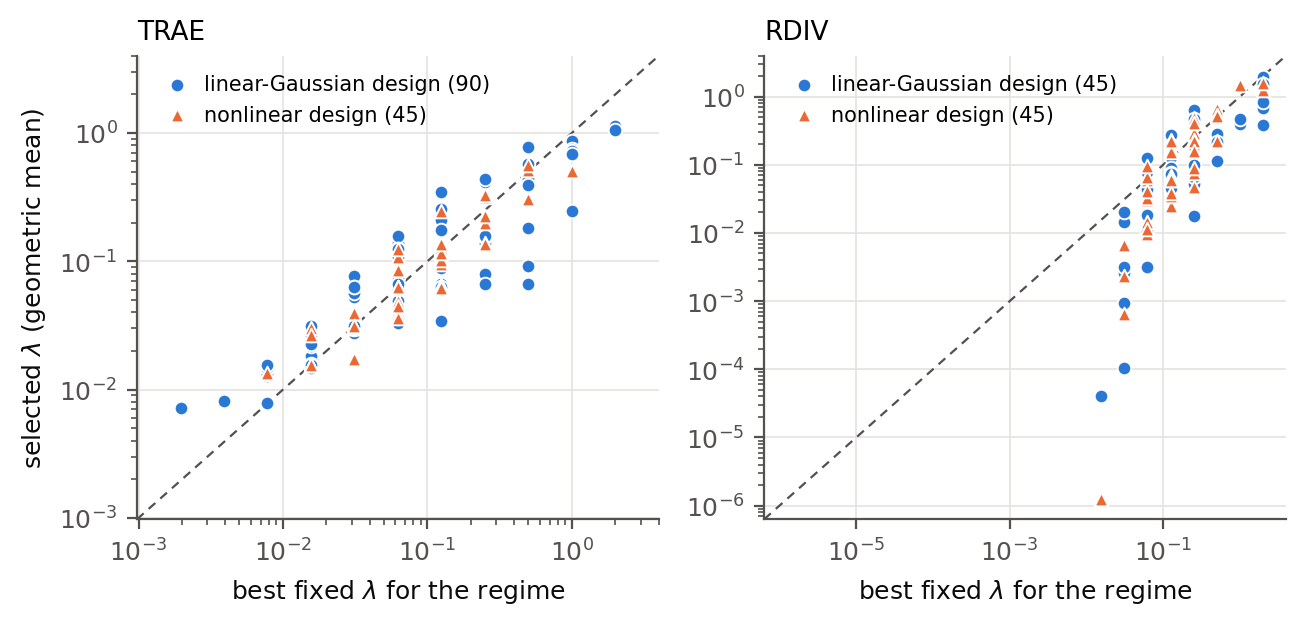
\includegraphics[width=0.9\linewidth]{kernel_tracking.png}
\caption{Selected penalty against the best fixed penalty for the strong error, one point per regime. The selected penalty is the geometric mean over the data sets of a regime. TRAE uses $90$ linear and $45$ nonlinear regimes; RDIV uses $45$ regimes of each design. The lowest RDIV points are regimes in which some searches reached the end of the grid. The dashed line is the diagonal.}
\label{fig:kernel_tracking}
\end{figure}

The fixed-scale rule is less accurate, with geometric mean ratios $1.24$ for the strong error and $1.59$ for the weak error. Its constant also matters: with constant $0.5$ or $2$ in place of one, the worst strong-error ratio becomes $14.8$ or $8.2$. The noise-floor rule has no such constant. At the threshold where the noise-floor rule stopped, the analytic $h_0$ would also have passed in $86\%$ of the data sets. The search never reached the end of the grid and accepted the initial value $\lambda_0=2$ in $3\%$ of the data sets. \Cref{fig:kernel_curves} shows the strong error against $n$ for $s=0.7$. The adaptive curve stays close to the best fixed penalty of each regime, while each fixed penalty is accurate only for some $(\rho,\sigma,n)$: $\lambda=2^{-1}$ at small $n$ and high noise, and $\lambda=2^{-9}$ at large $n$ and low noise.

\begin{figure}[!htp]
\centering
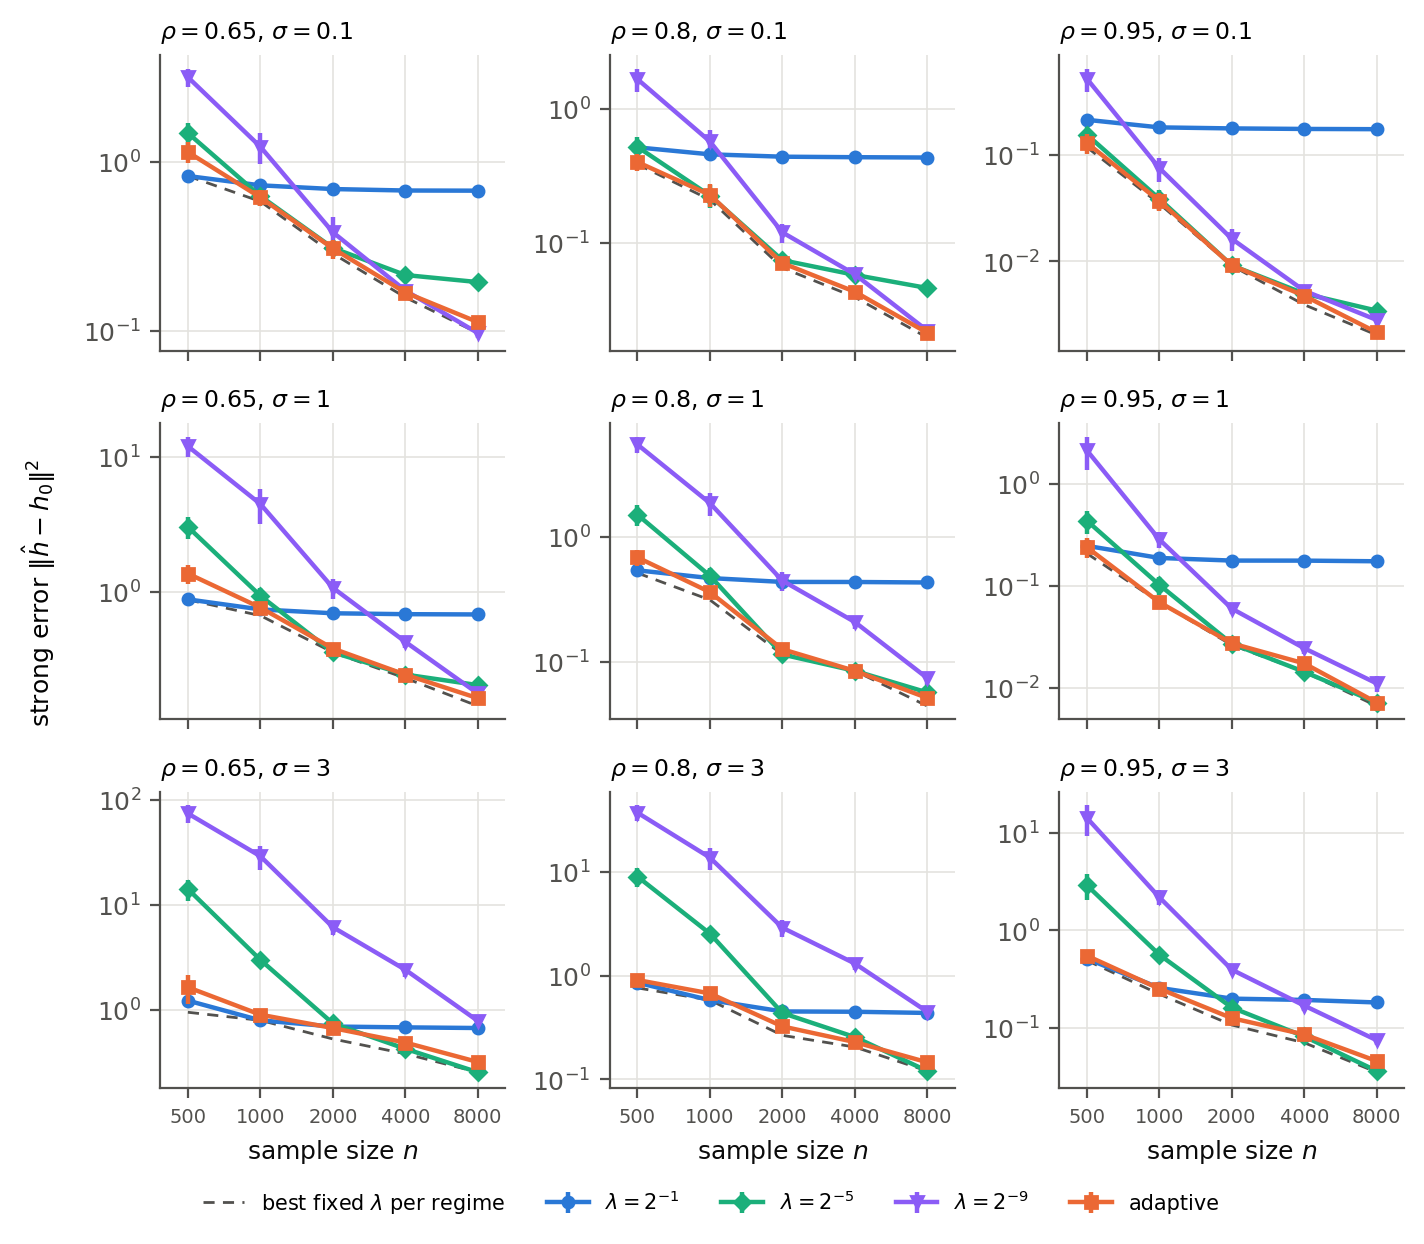
\includegraphics[width=\linewidth]{kernel_curves.png}
\caption{Strong error of TRAE against the sample size in the linear design with $s=0.7$, for three fixed penalties and the noise-floor rule. The dashed curve is the best fixed penalty of each regime. Bars show $\pm1$ Monte Carlo standard error over $50$ data sets.}
\label{fig:kernel_curves}
\end{figure}

\paragraph{Two designs, TRAE and RDIV.}
\Cref{tab:kernel_designs} adds the nonlinear design, RDIV, and the target error. TRAE improves on the best single fixed penalty in both designs and for all three errors. Its worst ratio is at most $2.19$, compared with $4.72$ to $13.43$ for the best single fixed penalty. Its smallest margin is for the weak error in the nonlinear design, $1.31$ against $1.41$.

RDIV improves on the best single fixed penalty in the linear design for all three errors. In the nonlinear design it improves the target error, $1.22$ against $1.40$, is close on the strong error, $1.30$ against $1.26$, and is worse on the weak error, $1.64$ against $1.23$. Its search is also less stable at both ends of the sample-size range. In the linear design it accepted $\lambda_0$ in $53\%$ of the data sets at $n=500$, and it reached the end of the grid in $7\%$ of the data sets overall and in $17\%$ to $20\%$ at $n=8000$, mostly at the lowest noise level. Two features of RDIV may explain the difference. It fits and calibrates on different blocks with an estimated operator, so its statistic need not decrease along the grid. It increased by more than $5\%$ in $18\%$ of the grid steps, while the TRAE statistic never did. Its noise floor also depends on the estimated operator error.

\begin{table}[!htp]
\centering
\caption{Geometric mean risk ratio over $45$ regimes per design, with the largest ratio in parentheses. The linear design uses $s=0.7$. ``Fixed'' is the best single fixed penalty, chosen after seeing the results, separately for each estimator, design, and error. The smaller geometric mean in each pair is in bold.}
\label{tab:kernel_designs}
\small
\setlength{\tabcolsep}{2.5pt}
\begin{tabular}{llcccccc}
\toprule
 & & \multicolumn{2}{c}{Strong error} & \multicolumn{2}{c}{Weak error} & \multicolumn{2}{c}{Target error}\\
\cmidrule(lr){3-4}\cmidrule(lr){5-6}\cmidrule(lr){7-8}
Estimator & Design & Adaptive & Fixed & Adaptive & Fixed & Adaptive & Fixed\\
\midrule
TRAE & Linear & $\mathbf{1.16}$ $(1.73)$ & $1.60$ $(7.78)$ & $\mathbf{1.24}$ $(1.90)$ & $1.59$ $(7.75)$ & $\mathbf{1.23}$ $(2.19)$ & $1.66$ $(13.43)$\\
 & Nonlinear & $\mathbf{1.07}$ $(1.30)$ & $1.48$ $(8.36)$ & $\mathbf{1.31}$ $(1.87)$ & $1.41$ $(4.72)$ & $\mathbf{1.12}$ $(1.80)$ & $1.58$ $(9.58)$\\
% Table spacing omitted for page compatibility.
RDIV & Linear & $\mathbf{1.34}$ $(3.69)$ & $1.43$ $(8.18)$ & $\mathbf{1.38}$ $(3.53)$ & $1.58$ $(12.93)$ & $\mathbf{1.39}$ $(7.81)$ & $1.56$ $(8.00)$\\
 & Nonlinear & $1.30$ $(2.61)$ & $\mathbf{1.26}$ $(3.57)$ & $1.64$ $(2.62)$ & $\mathbf{1.23}$ $(3.36)$ & $\mathbf{1.22}$ $(2.60)$ & $1.40$ $(7.90)$\\
\bottomrule
\end{tabular}
\end{table}

\paragraph{Scope.}
We chose the regimes so that the best penalty changes across them, since this is the setting in which a tuning rule is needed. Within a single regime, the best fixed penalty for that regime is about as accurate as the rule, and usually more accurate. The Gaussian designs violate the boundedness conditions of our theorems, and the noise-floor rule uses a data-driven $A_n$. The experiments therefore show how the rule behaves with exact penalized solutions under conditions that the theory does not cover.

\section{Conclusion}

We develop a discrepancy rule for choosing the regularization level in conditional moment models when the source smoothness is unknown. The rule sets its threshold from prescribed bounds on statistical error and applies to both RDIV and TRAE. Its oracle guarantee reduces the analysis of any such rule to two ingredients: a discrepancy bound and weak- and strong-error bounds, both holding at every grid point. This general principle applies to the noniterative and iterative versions of RDIV and TRAE, and it yields adaptive rates that match known-smoothness comparisons within the smoothness ranges stated in the theorems when the underlying statistical errors are comparable. The threshold still requires valid statistical-error bounds. In simulations with kernel classes, where every candidate is an exact penalized solution, the rule followed the best fixed penalty across settings in which that penalty changed by three orders of magnitude, and it stayed close to the best penalty of each setting. These results use a data-driven noise level. A calibration of the noise level that the theory covers, and the role of optimization error for neural network classes, remain open.

\bibliography{reference.bib}
\bibliographystyle{plainnat}

\newpage

\appendix 

\section{Proof of the General Oracle Guarantee}\label{sec:proof_common_dp}

\begin{proof}[Proof of \cref{thm:common_dp}]
The proof has three steps. First, we prove that the oracle point is always accepted.  The rule therefore stops no later than that point, and acceptance together with monotonicity turns the error bounds into the stated rates.

First, by \eqref{eq:common_discrepancy_bound} and
\eqref{eq:common_oracle_crossing},
\[
D_n(\hat h_{\lambda^\circ})
\leqslant A_n(\lambda^\circ)
+B_n(\lambda^\circ)
\leqslant\frac32 A_n(\lambda^\circ).
\]
Thus $\lambda^\circ$ is accepted, so some candidate clears its threshold and the fallback is not reached. Second, since \cref{alg:discrepancy} searches from larger to smaller regularization and stops at the first acceptance, it returns a point
$\lambda_{\mathrm{dp}}\geqslant\lambda^\circ$.
Third, every grid point between $\lambda^\circ$ and $2$ lies in $\mathcal S_n$, so
\eqref{eq:common_accepted_bounds} applies at the selected point. The rule accepted
$\lambda_{\mathrm{dp}}$, so $D_n(\hat h_{\lambda_{\mathrm{dp}}})\leqslant\tfrac32A_n(\lambda_{\mathrm{dp}})$ and
\[
D_n(\hat h_{\lambda_{\mathrm{dp}}})+A_n(\lambda_{\mathrm{dp}})
\leqslant\frac52 A_n(\lambda_{\mathrm{dp}}).
\]
Because $A_n$ is nonincreasing over the grid points in $[\lambda^\circ,2]$ and $\lambda\mapsto1/\lambda$ decreases, the product $A_n(\lambda)/\lambda$ is nonincreasing there as well, so
\[
A_n(\lambda_{\mathrm{dp}})
\leqslant A_n(\lambda^\circ),
\qquad
\frac{A_n(\lambda_{\mathrm{dp}})}{\lambda_{\mathrm{dp}}}
\leqslant\frac{A_n(\lambda^\circ)}{\lambda^\circ}.
\]
Substituting the last two displays into \eqref{eq:common_accepted_bounds} proves
\eqref{eq:common_rate}.
\end{proof}

The following consequence of the source condition allows us to compare
both one-step estimators directly with $h_0$.

\begin{lemma}[Variational source inequality]\label{lemma:variational_source}
Let $\mathcal A=\mathcal T^*\mathcal T$,
$b=\min\{\beta,1\}$, $p=1+b$, and $\alpha=b/(1+b)$. Under
\cref{asp:source_condition}, every $u\in\widetilde{\mathcal H}$ satisfies
\[
|\langle h_0,u\rangle|
\leqslant \|w_0\|\,\|\mathcal Tu\|^b\|u\|^{1-b}.
\]
Consequently, for every fixed $\epsilon\in(0,1)$ and
$\lambda\in(0,2]$,
\begin{align*}
2\lambda|\langle h_0,u\rangle|
&\leqslant
\epsilon\{\|\mathcal Tu\|^2+\lambda\|u\|^2\}
+C_\epsilon\|w_0\|^2\lambda^p,\\
2|\langle h_0,u\rangle|
&\leqslant
\epsilon\|u\|^2
+C_\epsilon\|w_0\|^{2/(1+b)}
\|\mathcal Tu\|^{2b/(1+b)}.
\end{align*}
\end{lemma}

\begin{proof}
For $0<\beta\leqslant1$, spectral interpolation and
$\|\mathcal A\|\leqslant1$ give
\[
|\langle h_0,u\rangle|
=|\langle w_0,\mathcal A^{\beta/2}u\rangle|
\leqslant
\|w_0\|\,\|\mathcal A^{1/2}u\|^\beta\|u\|^{1-\beta}.
\]
For $\beta>1$, the positive self-adjoint operator $\mathcal A$ has spectrum
in $[0,1]$ because $\|\mathcal A\|\leqslant1$. Let $\mu_u$ denote its
spectral measure associated with $u$. Since $s^\beta\leqslant s$ for
$s\in[0,1]$,
\[
\|\mathcal A^{\beta/2}u\|^2
=\int_{[0,1]}s^\beta\,d\mu_u(s)
\leqslant\int_{[0,1]}s\,d\mu_u(s)
=\|\mathcal A^{1/2}u\|^2.
\]
Since $\|\mathcal A^{1/2}u\|=\|\mathcal Tu\|$, these two cases prove
the first display. To obtain the first consequence, set
$E_\lambda=\|\mathcal Tu\|^2+\lambda\|u\|^2$ and observe that
\[
2\lambda|\langle h_0,u\rangle|
\leqslant 2\|w_0\|\lambda^{(1+b)/2}E_\lambda^{1/2}.
\]
The inequality $2uv\leqslant\epsilon u^2+\epsilon^{-1}v^2$ gives the first consequence with $C_\epsilon=\epsilon^{-1}$, uniformly over $b\in(0,1]$. Its coefficient is independent of $\beta$ and $\|w_0\|$. Applying the weighted form
of the same inequality to
$2\|w_0\|\|\mathcal Tu\|^b\|u\|^{1-b}$ gives the second consequence.
\end{proof}

\section[Proofs for RDIV]{Proofs of \cref{sec:rdiv}}

Throughout the appendix, $R^\lambda(h)=L(h)+\lambda\|h\|^2$ and
$R_n^\lambda(h)=L_n(h)+\lambda\|h\|_{2,n}^2$, where
\[
\|h\|_{2,n}:=\{\mathbb E_n[h(X)^2]\}^{1/2}.
\]
In this section, $\mathbb E_n$ is the average on $I_{\mathrm{fit}}$,
$L(h)=\sigma^2_{Y\mid Z}+\|\mathcal T(h-h_0)\|^2$, and $D_n$ is the projected discrepancy in \eqref{eq:rdiv_projected_loss}. We use the scales in \eqref{eq:delta_deepiv}. Constants may depend on the fixed bounds and population quantities; they are uniform over $n$ and the regularization grid.

\begin{lemma}[Preliminary RDIV nuisance and operator bounds]\label{lemma:t_err_dp}
Under \cref{asp:re_cd,asp:cr_deepiv}, with probability at least $1-\xi$,
\begin{align}
\mathbb E_Z\!\left[H^2\{\hat g(\cdot\mid Z),g_0(\cdot\mid Z)\}\right]
&\leqslant C\delta_{n,\mathcal G}^2,
\label{eq:rdiv_mle_hellinger}\\
\|\hat r-r_0\|_{L_2(Z)}&\leqslant \delta_{n,r},\nonumber\\
\sup_{h\in\mathcal H}
\|(\hat{\mathcal T}-\mathcal T)h\|_{L_2(Z)}
&\leqslant C\delta_{n,\mathcal G},\label{eq:rdiv_op_global}\\
\|(\hat{\mathcal T}-\mathcal T)(h-h')\|_{L_1(Z)}
&\leqslant C\delta_{n,\mathcal G}\|h-h'\|,
\qquad h,h'\in\mathcal H.\label{eq:rdiv_op_relative}
\end{align}
Moreover, if
\[
\widehat L(h):=\mathbb E[(Y-\hat{\mathcal T}h(Z))^2\mid I_{\mathrm{pre}}],
\]
then, uniformly over $h,h'\in\mathcal H$,
\begin{equation}\label{eq:rdiv_first_stage_loss}
|\{\widehat L(h)-\widehat L(h')\}-\{L(h)-L(h')\}| \leqslant C\delta_{n,\mathcal G}\|h-h'\|.
\end{equation}

\emph{Additional conditions.} For the conditional fitting argument in Lemma~\ref{lemma:err_l_dp}, use the following measurable-version convention. Let $Q$ denote the law of one observation $W$, let $a$ denote the preliminary observations, and put $Q_n^{\mathbf w}=n^{-1}\sum_{i=1}^n\delta_{w_i}$ for a fresh fitting tuple $\mathbf w=(w_1,\ldots,w_n)$. Define \[ \ell_{\lambda,a}(h;w)=\{Y(w)-(\hat{\mathcal T}_a h)(Z(w))\}^2+\lambda h(X(w))^2, \qquad S_{n,\lambda,q}(a,\mathbf w)=\sup_{\substack{h\in\mathcal H\\\|h-h_0\|\leqslant q}}\left|(Q_n^{\mathbf w}-Q)\{\ell_{\lambda,a}(h)-\ell_{\lambda,a}(h_0)\}\right|. \] For each $n\geqslant1$, $\lambda\in\Lambda_n$ and positive rational $q$, $S_{n,\lambda,q}$ admits an extended nonnegative version jointly measurable in the preliminary observations and the fresh fitting tuple. This version agrees with $S_{n,\lambda,q}(a,\cdot)$ for $Q^n$-almost every tuple for almost every preliminary realization, and agrees almost surely with $S_{n,\lambda,q}(I_{\mathrm{pre}},(W_i)_{i\in I_{\mathrm{fit}}})$ at the actual independent fitting block. All losses use the same function representatives as the empirical objective. This is only a measurability and evaluation-coherence convention; no deviation bound, rate, countability or separability is assumed. For the fitted conditional density in the RDIV preliminary construction, use a coherent measurable version at independent calibration observations. For each $n\geqslant1$, writing $a=I_{\mathrm{pre}}$, the selected density $\hat g_{n,a}(x\mid z)$ admits a nonnegative version $\bar g_n(a,x,z)$ jointly measurable in the preliminary observations, $x$ and $z$. For almost every preliminary realization $a$, for $P_Z$-almost every $z$, the functions $\bar g_n(a,\cdot,z)$ and $\hat g_{n,a}(\cdot\mid z)$ agree $\mu$-almost everywhere. Almost surely, this same agreement holds at every actual calibration observation $Z_i$, $i\in I_{\mathrm{cal}}$. The empirical objectives and selected maximizer remain those defined using the original supplied representatives: this convention does not replace the optimizer. It supplies only measurability and coherence of the fitted density evaluated on the independent calibration sample; it assumes no normalization event, probability inequality, rate, countability or separability. For the preliminary regression estimate used in the RDIV calibration loss, take a coherent measurable version on the independent calibration sample. For each $n\geqslant1$, writing $a=I_{\mathrm{pre}}$, the selected $L_2(Z)$ pilot has a version $\bar r_n(a,z)$ jointly measurable in the preliminary observations and $z$. For almost every preliminary realization $a$, $\bar r_n(a,z)=\hat r_{n,a}(z)$ for $P_Z$-almost every $z$. Almost surely, the same equality holds simultaneously at every actual calibration observation $Z_i$, $i\in I_{\mathrm{cal}}$, for the supplied representatives used in $D_n$. This is only a measurability and evaluation-coherence convention. It imposes no exact joint measurability on every supplied representative, does not replace an empirical objective or selected optimizer, and supplies no boundedness event, probability inequality, error rate, countability or separability assumption. The existing pilot accuracy and envelope assumptions remain unchanged. Use the following well-definedness convention for the likelihood-transform critical-radius and concentration arguments in Assumption~\ref{asp:cr_deepiv} and Lemma~\ref{lemma:t_err_dp}, separately from the existing hypothesis-class, density-image and fitted-process conventions. Let $Q$ be the true joint law of $(X,Z)$, let $\mathcal G_0$ be the likelihood-transform class already defined in Assumption~\ref{asp:cr_deepiv}, and put \[ \mathcal A_r=\{f\in\operatorname{star}(\mathcal G_0-\mathcal G_0):\|f\|_{L_2(Q)}\leqslant r\}. \] For every integer $n\geqslant1$ and every $r>0$, the three processes \[ \sup_{f\in\mathcal G_0}|(Q_n-Q)f|,\qquad \sup_{f\in\mathcal A_r}|(Q_n-Q)f|,\qquad \sup_{f\in\mathcal A_r}\left|\frac1n\sum_{i=1}^n\epsilon_i f(X_i,Z_i)\right| \] regarded as extended nonnegative quantities, are measurable under $Q^n$ for the first two and under the product of $Q^n$ with the independent Rademacher law for the third. The functions use the same fixed density representatives as the likelihood objective. This convention only makes these empirical processes and their expectations well defined. It supplies no concentration event, deviation inequality, probability bound, rate, countability, separability, or additional statistical restriction.
\end{lemma}

\emph{Additional condition.} For another result of the paper: Use the following well-definedness convention for the likelihood-transform critical-radius and concentration arguments in Assumption~\ref{asp:cr_deepiv} and Lemma~\ref{lemma:t_err_dp}, separately from the existing hypothesis-class, density-image and fitted-process conventions. Let $Q$ be the true joint law of $(X,Z)$, let $\mathcal G_0$ be the likelihood-transform class already defined in Assumption~\ref{asp:cr_deepiv}, and put \[ \mathcal A_r=\{f\in\operatorname{star}(\mathcal G_0-\mathcal G_0):\|f\|_{L_2(Q)}\leqslant r\}. \] For every integer $n\geqslant1$ and every $r>0$, the three processes \[ \sup_{f\in\mathcal G_0}|(Q_n-Q)f|,\qquad \sup_{f\in\mathcal A_r}|(Q_n-Q)f|,\qquad \sup_{f\in\mathcal A_r}\left|\frac1n\sum_{i=1}^n\epsilon_i f(X_i,Z_i)\right| \] regarded as extended nonnegative quantities, are measurable under $Q^n$ for the first two and under the product of $Q^n$ with the independent Rademacher law for the third. The functions use the same fixed density representatives as the likelihood objective. This convention only makes these empirical processes and their expectations well defined. It supplies no concentration event, deviation inequality, probability bound, rate, countability, separability, or additional statistical restriction.

\noindent\textit{Remark (notation).} $H^2(g_1,g_2)=\int(\sqrt{g_1(x)}-\sqrt{g_2(x)})^2\,\mu(dx)$ is defined for probability densities $g_1,g_2$ with respect to the common measure $\mu$ on $\mathcal X$; for conditional densities it is evaluated at each fixed $z$, with any averaging over $Z$ written separately.

\begin{proof}
Allocate failure probability $\xi/2$ to the conditional-density estimator and
$\xi/2$ to the pilot regression. As elsewhere, evaluate the corresponding
deterministic accuracy bounds at these confidence levels and relabel them
$\delta_{n,\mathcal G}$ and $\delta_{n,r}$.
We establish the density bound directly using the Localized Concentration lemma of \citet{li2024regularized}. Write $P=\mathbb E_{X,Z}$ and $P_n=\mathbb E_{n,\mathrm{pre}}$, and define

\[
f_g(x,z)=\sqrt{\frac{g(x\mid z)+g_0(x\mid z)}{2g_0(x\mid z)}},\qquad
\mathcal U=\{f_g-1:g\in\mathcal G\}.
\]

Realizability gives $f_{g_0}=1$, so $0\in\mathcal U$. The density bounds give

\[
2^{-1/2}\leqslant f_g\leqslant M,\qquad
M=\sqrt{\frac{C_G/c_0+1}{2}}.
\]

Thus $\mathcal U$ is uniformly bounded by a fixed constant. Define the globally Lipschitz loss

\[
\ell(v)=-\log\bigl(\max\{1+v,2^{-1/2}\}\bigr).
\]

The maximum map is $1$-Lipschitz, and the derivative of $-\log t$ has absolute value at most $\sqrt2$ for $t\geqslant2^{-1/2}$. Hence $\ell$ is $\sqrt2$-Lipschitz, $\ell(0)=0$, and $\ell(f_g-1)=-\log f_g$. 

We verify the localized complexity condition for this application. Put $\mathcal S=\operatorname{star}(\mathcal G_0-\mathcal G_0)$ and choose a deterministic critical radius $d\leqslant\delta_{n,\mathcal G}$ as supplied by Assumption~\ref{asp:cr_deepiv}. By the critical-radius definition, $\mathfrak R_n(d;\mathcal S)\leqslant d^2$. For $s\geqslant d$, star-shapedness implies that $(d/s)v\in\mathcal S$ and $\|(d/s)v\|_{L_2(X,Z)}\leqslant d$ whenever $v\in\mathcal S$ and $\|v\|_{L_2(X,Z)}\leqslant s$. Scaling inside the Rademacher supremum therefore gives

\[
\mathfrak R_n(s;\mathcal S)
\leqslant\frac{s}{d}\mathfrak R_n(d;\mathcal S)
\leqslant sd.
\]

Since $1\in\mathcal G_0$, we have $\operatorname{star}(\mathcal U)\subseteq\mathcal S$. Taking $s=\delta_{n,\mathcal G}$ yields

\[
\mathfrak R_n\bigl(\delta_{n,\mathcal G};\operatorname{star}(\mathcal U)\bigr)
\leqslant\delta_{n,\mathcal G}d
\leqslant\delta_{n,\mathcal G}^2.
\]

Apply the cited localized concentration lemma with input $(X,Z)$, one coordinate, class $\mathcal U$, fixed comparator $0$, loss $\ell$, and failure probability $\xi/2$. The measurability and logarithmic radius floor are supplied by Assumption~\ref{asp:cr_deepiv}, with the confidence evaluation specified in the proof. Consequently, for a fixed constant $A>0$, with probability at least $1-\xi/2$,

\[
\left|(P_n-P)(-\log f_g)\right|
\leqslant A\left\{\delta_{n,\mathcal G}\|f_g-1\|_{L_2(X,Z)}+\delta_{n,\mathcal G}^2\right\},
\qquad g\in\mathcal G.
\]
 

To use empirical optimality, note that $P_n\log g_0(X\mid Z)$ is finite by the density bounds. Since $\hat g$ maximizes the empirical log likelihood and all candidate densities are bounded above, $\hat g(X_i\mid Z_i)>0$ at every preliminary observation, almost surely. For $a>0$, the arithmetic-geometric mean inequality gives $(a+1)/2\geqslant\sqrt a$, and hence

\[
-\log\sqrt{\frac{a+1}{2}}\leqslant-\frac14\log a.
\]

Taking $a=\hat g(X_i\mid Z_i)/g_0(X_i\mid Z_i)$ and averaging gives

\[
P_n(-\log f_{\hat g})
\leqslant-\frac14P_n\log\frac{\hat g(X\mid Z)}{g_0(X\mid Z)}
\leqslant0.
\]

For every $g\in\mathcal G$, conditional density normalization gives

\[
P f_g^2
=\mathbb E_Z\int\frac{g(x\mid Z)+g_0(x\mid Z)}2\,\mu(dx)=1.
\]

Since $\log t\leqslant t-1$ for $t>0$, it follows that

\[
P(-\log f_g)\geqslant1-Pf_g
=\frac12P(f_g-1)^2.
\]

On the concentration event, put $b=\|f_{\hat g}-1\|_{L_2(X,Z)}$. Combining these inequalities and using Young's inequality gives

\[
\frac{b^2}{2}
\leqslant P(-\log f_{\hat g})
\leqslant A\delta_{n,\mathcal G}b+A\delta_{n,\mathcal G}^2
\leqslant\frac{b^2}{4}+(A^2+A)\delta_{n,\mathcal G}^2.
\]

Thus $b^2\leqslant4(A^2+A)\delta_{n,\mathcal G}^2$. 

Finally, for $t\geqslant0$ and $f=\sqrt{(t^2+1)/2}$, we have $f\leqslant t+1$ and

\[
|t-1|=\frac{2(f+1)}{t+1}|f-1|\leqslant4|f-1|.
\]

Apply this pointwise with $t=\sqrt{\hat g/g_0}$ and integrate under the true joint distribution to obtain

\[
\begin{aligned}
\mathbb E_Z\!\left[H^2\{\hat g(\cdot\mid Z),g_0(\cdot\mid Z)\}\right]
&=P\left(\sqrt{\frac{\hat g(X\mid Z)}{g_0(X\mid Z)}}-1\right)^2\\
&\leqslant16b^2
\leqslant64(A^2+A)\delta_{n,\mathcal G}^2.
\end{aligned}
\]

This proves \eqref{eq:rdiv_mle_hellinger} with probability at least $1-\xi/2$. The
nuisance-rate assumption gives
$\|\hat r-r_0\|_{L_2(Z)}\leqslant\delta_{n,r}$ with probability at least
$1-\xi/2$. Therefore, without requiring independence between $\hat g$ and
$\hat r$, the union bound shows that both inequalities hold simultaneously
with probability at least $1-\xi$. We work on this intersection for
the rest of the proof. Here
\[
H^2(g_1,g_2)=\int\{\sqrt{g_1(x)}-\sqrt{g_2(x)}\}^2\,\mu(dx).
\]

Let $P_X$ be the true marginal distribution of $X$ and let $\hat P_X$ be the marginal induced by $Z\sim P_Z$ and $X\mid Z\sim\hat g(\cdot\mid Z)$. The density bounds in \cref{asp:re_cd} give $\hat g(x\mid z)/g_0(x\mid z)\leqslant C_G/c_0$ and hence
\[
\frac{d\hat P_X}{dP_X}\leqslant \frac{C_G}{c_0}.
\]
The total-variation--Hellinger inequality and $\|h\|_\infty\leqslant B$ give
\[
\|(\hat{\mathcal T}-\mathcal T)h\|^2
\leqslant B^2\mathbb E_Z
\left[\left\{\int|\hat g(x\mid Z)-g_0(x\mid Z)|\,\mu(dx)\right\}^2\right]
\leqslant C B^2\delta_{n,\mathcal G}^2,
\]
which proves \eqref{eq:rdiv_op_global}. For $u=h-h'$, factor
$\hat g/g_0-1=(\sqrt{\hat g/g_0}-1)(\sqrt{\hat g/g_0}+1)$.
Cauchy--Schwarz and the conditional density-ratio bound yield
\begin{align*}
\|(\hat{\mathcal T}-\mathcal T)u\|_1
&\leqslant
\mathbb E\left[|u(X)|
\left|\sqrt{\frac{\hat g(X\mid Z)}{g_0(X\mid Z)}}-1\right|
\left\{\sqrt{\frac{\hat g(X\mid Z)}{g_0(X\mid Z)}}+1\right\}\right]\\
&\leqslant C\|u\|
\mathbb E_Z\!\left[H^2\{\hat g(\cdot\mid Z),g_0(\cdot\mid Z)\}\right]^{1/2}
\leqslant C\delta_{n,\mathcal G}\|u\|,
\end{align*}
which proves \eqref{eq:rdiv_op_relative}. \citet{li2024regularized} use the same operator argument in their MLE analysis.

Finally, write $e_h=(\hat{\mathcal T}-\mathcal T)h$. Pointwise,
\begin{align*}
&(Y-\hat{\mathcal T}h)^2-(Y-\hat{\mathcal T}h')^2
-\{(Y-\mathcal T h)^2-(Y-\mathcal T h')^2\}\\
&\quad=-(\hat{\mathcal T}-\mathcal T)u
(2Y-\hat{\mathcal T}h-\hat{\mathcal T}h')
+\mathcal T u(e_h+e_{h'}).
\end{align*}
The expectation of the first term is at most
$4B\|(\hat{\mathcal T}-\mathcal T)u\|_1$; the second is at most
$\|\mathcal T u\|(\|e_h\|+\|e_{h'}\|)$. Apply
\eqref{eq:rdiv_op_global}, \eqref{eq:rdiv_op_relative}, and conditional Jensen to obtain \eqref{eq:rdiv_first_stage_loss}.
\end{proof}

\begin{lemma}[Uniform RDIV empirical comparisons]\label{lemma:err_l_dp}
Under \cref{asp:range,asp:closeness_deepiv,asp:re_cd,asp:cr_deepiv}, there is an event $\mathcal E_n^{\mathrm R}$ with probability at least $1-\xi$ on which, simultaneously for every $\lambda\in\Lambda_n$ and $h\in\mathcal H$,
\begin{align}
&\left|\{\widehat R^\lambda(h)-\widehat R^\lambda(h_0)\}
-\{R_n^\lambda(h)-R_n^\lambda(h_0)\}\right|
\leqslant C\{\delta_{n,\mathcal H}\|h-h_0\|
+\delta_{n,\mathcal H}^2\},\label{eq:rdiv_fit_comparison}\\
&\left|D_n(\hat h_\lambda)
-\|\mathcal T(\hat h_\lambda-h_0)\|^2\right|
\leqslant C\nu_n\|\mathcal T(\hat h_\lambda-h_0)\|+C\nu_n^2,
\label{eq:rdiv_projected_comparison}
\end{align}
where $\widehat R^\lambda(h)=\widehat L(h)+\lambda\|h\|^2$.

\emph{Additional conditions.} For the conditional fitting argument in Lemma~\ref{lemma:err_l_dp}, use the following measurable-version convention. Let $Q$ denote the law of one observation $W$, let $a$ denote the preliminary observations, and put $Q_n^{\mathbf w}=n^{-1}\sum_{i=1}^n\delta_{w_i}$ for a fresh fitting tuple $\mathbf w=(w_1,\ldots,w_n)$. Define \[ \ell_{\lambda,a}(h;w)=\{Y(w)-(\hat{\mathcal T}_a h)(Z(w))\}^2+\lambda h(X(w))^2, \qquad S_{n,\lambda,q}(a,\mathbf w)=\sup_{\substack{h\in\mathcal H\\\|h-h_0\|\leqslant q}}\left|(Q_n^{\mathbf w}-Q)\{\ell_{\lambda,a}(h)-\ell_{\lambda,a}(h_0)\}\right|. \] For each $n\geqslant1$, $\lambda\in\Lambda_n$ and positive rational $q$, $S_{n,\lambda,q}$ admits an extended nonnegative version jointly measurable in the preliminary observations and the fresh fitting tuple. This version agrees with $S_{n,\lambda,q}(a,\cdot)$ for $Q^n$-almost every tuple for almost every preliminary realization, and agrees almost surely with $S_{n,\lambda,q}(I_{\mathrm{pre}},(W_i)_{i\in I_{\mathrm{fit}}})$ at the actual independent fitting block. All losses use the same function representatives as the empirical objective. This is only a measurability and evaluation-coherence convention; no deviation bound, rate, countability or separability is assumed. For the fitted conditional density in the RDIV preliminary construction, use a coherent measurable version at independent calibration observations. For each $n\geqslant1$, writing $a=I_{\mathrm{pre}}$, the selected density $\hat g_{n,a}(x\mid z)$ admits a nonnegative version $\bar g_n(a,x,z)$ jointly measurable in the preliminary observations, $x$ and $z$. For almost every preliminary realization $a$, for $P_Z$-almost every $z$, the functions $\bar g_n(a,\cdot,z)$ and $\hat g_{n,a}(\cdot\mid z)$ agree $\mu$-almost everywhere. Almost surely, this same agreement holds at every actual calibration observation $Z_i$, $i\in I_{\mathrm{cal}}$. The empirical objectives and selected maximizer remain those defined using the original supplied representatives: this convention does not replace the optimizer. It supplies only measurability and coherence of the fitted density evaluated on the independent calibration sample; it assumes no normalization event, probability inequality, rate, countability or separability. For the preliminary regression estimate used in the RDIV calibration loss, take a coherent measurable version on the independent calibration sample. For each $n\geqslant1$, writing $a=I_{\mathrm{pre}}$, the selected $L_2(Z)$ pilot has a version $\bar r_n(a,z)$ jointly measurable in the preliminary observations and $z$. For almost every preliminary realization $a$, $\bar r_n(a,z)=\hat r_{n,a}(z)$ for $P_Z$-almost every $z$. Almost surely, the same equality holds simultaneously at every actual calibration observation $Z_i$, $i\in I_{\mathrm{cal}}$, for the supplied representatives used in $D_n$. This is only a measurability and evaluation-coherence convention. It imposes no exact joint measurability on every supplied representative, does not replace an empirical objective or selected optimizer, and supplies no boundedness event, probability inequality, error rate, countability or separability assumption. The existing pilot accuracy and envelope assumptions remain unchanged. Use the following well-definedness convention for the likelihood-transform critical-radius and concentration arguments in Assumption~\ref{asp:cr_deepiv} and Lemma~\ref{lemma:t_err_dp}, separately from the existing hypothesis-class, density-image and fitted-process conventions. Let $Q$ be the true joint law of $(X,Z)$, let $\mathcal G_0$ be the likelihood-transform class already defined in Assumption~\ref{asp:cr_deepiv}, and put \[ \mathcal A_r=\{f\in\operatorname{star}(\mathcal G_0-\mathcal G_0):\|f\|_{L_2(Q)}\leqslant r\}. \] For every integer $n\geqslant1$ and every $r>0$, the three processes \[ \sup_{f\in\mathcal G_0}|(Q_n-Q)f|,\qquad \sup_{f\in\mathcal A_r}|(Q_n-Q)f|,\qquad \sup_{f\in\mathcal A_r}\left|\frac1n\sum_{i=1}^n\epsilon_i f(X_i,Z_i)\right| \] regarded as extended nonnegative quantities, are measurable under $Q^n$ for the first two and under the product of $Q^n$ with the independent Rademacher law for the third. The functions use the same fixed density representatives as the likelihood objective. This convention only makes these empirical processes and their expectations well defined. It supplies no concentration event, deviation inequality, probability bound, rate, countability, separability, or additional statistical restriction.
\end{lemma}

\emph{Additional conditions.} For a result cited in the proof of Lemma~\ref{lemma:err_l_dp}: For the conditional fitting argument in Lemma~\ref{lemma:err_l_dp}, use the following measurable-version convention. Let $Q$ denote the law of one observation $W$, let $a$ denote the preliminary observations, and put $Q_n^{\mathbf w}=n^{-1}\sum_{i=1}^n\delta_{w_i}$ for a fresh fitting tuple $\mathbf w=(w_1,\ldots,w_n)$. Define \[ \ell_{\lambda,a}(h;w)=\{Y(w)-(\hat{\mathcal T}_a h)(Z(w))\}^2+\lambda h(X(w))^2, \qquad S_{n,\lambda,q}(a,\mathbf w)=\sup_{\substack{h\in\mathcal H\\\|h-h_0\|\leqslant q}}\left|(Q_n^{\mathbf w}-Q)\{\ell_{\lambda,a}(h)-\ell_{\lambda,a}(h_0)\}\right|. \] For each $n\geqslant1$, $\lambda\in\Lambda_n$ and positive rational $q$, $S_{n,\lambda,q}$ admits an extended nonnegative version jointly measurable in the preliminary observations and the fresh fitting tuple. This version agrees with $S_{n,\lambda,q}(a,\cdot)$ for $Q^n$-almost every tuple for almost every preliminary realization, and agrees almost surely with $S_{n,\lambda,q}(I_{\mathrm{pre}},(W_i)_{i\in I_{\mathrm{fit}}})$ at the actual independent fitting block. All losses use the same function representatives as the empirical objective. This is only a measurability and evaluation-coherence convention; no deviation bound, rate, countability or separability is assumed. For a result cited in the proof of Lemma~\ref{lemma:err_l_dp}: For the fitted conditional density in the RDIV preliminary construction, use a coherent measurable version at independent calibration observations. For each $n\geqslant1$, writing $a=I_{\mathrm{pre}}$, the selected density $\hat g_{n,a}(x\mid z)$ admits a nonnegative version $\bar g_n(a,x,z)$ jointly measurable in the preliminary observations, $x$ and $z$. For almost every preliminary realization $a$, for $P_Z$-almost every $z$, the functions $\bar g_n(a,\cdot,z)$ and $\hat g_{n,a}(\cdot\mid z)$ agree $\mu$-almost everywhere. Almost surely, this same agreement holds at every actual calibration observation $Z_i$, $i\in I_{\mathrm{cal}}$. The empirical objectives and selected maximizer remain those defined using the original supplied representatives: this convention does not replace the optimizer. It supplies only measurability and coherence of the fitted density evaluated on the independent calibration sample; it assumes no normalization event, probability inequality, rate, countability or separability. For a result cited in the proof of Lemma~\ref{lemma:err_l_dp}: For the preliminary regression estimate used in the RDIV calibration loss, take a coherent measurable version on the independent calibration sample. For each $n\geqslant1$, writing $a=I_{\mathrm{pre}}$, the selected $L_2(Z)$ pilot has a version $\bar r_n(a,z)$ jointly measurable in the preliminary observations and $z$. For almost every preliminary realization $a$, $\bar r_n(a,z)=\hat r_{n,a}(z)$ for $P_Z$-almost every $z$. Almost surely, the same equality holds simultaneously at every actual calibration observation $Z_i$, $i\in I_{\mathrm{cal}}$, for the supplied representatives used in $D_n$. This is only a measurability and evaluation-coherence convention. It imposes no exact joint measurability on every supplied representative, does not replace an empirical objective or selected optimizer, and supplies no boundedness event, probability inequality, error rate, countability or separability assumption. The existing pilot accuracy and envelope assumptions remain unchanged. For a result cited in the proof of Lemma~\ref{lemma:err_l_dp}: Use the following well-definedness convention for the likelihood-transform critical-radius and concentration arguments in Assumption~\ref{asp:cr_deepiv} and Lemma~\ref{lemma:t_err_dp}, separately from the existing hypothesis-class, density-image and fitted-process conventions. Let $Q$ be the true joint law of $(X,Z)$, let $\mathcal G_0$ be the likelihood-transform class already defined in Assumption~\ref{asp:cr_deepiv}, and put \[ \mathcal A_r=\{f\in\operatorname{star}(\mathcal G_0-\mathcal G_0):\|f\|_{L_2(Q)}\leqslant r\}. \] For every integer $n\geqslant1$ and every $r>0$, the three processes \[ \sup_{f\in\mathcal G_0}|(Q_n-Q)f|,\qquad \sup_{f\in\mathcal A_r}|(Q_n-Q)f|,\qquad \sup_{f\in\mathcal A_r}\left|\frac1n\sum_{i=1}^n\epsilon_i f(X_i,Z_i)\right| \] regarded as extended nonnegative quantities, are measurable under $Q^n$ for the first two and under the product of $Q^n$ with the independent Rademacher law for the third. The functions use the same fixed density representatives as the likelihood objective. This convention only makes these empirical processes and their expectations well defined. It supplies no concentration event, deviation inequality, probability bound, rate, countability, separability, or additional statistical restriction.

\noindent\textit{Remark (notation).} $\mathcal E_n^{\mathrm R}$ is the intersection of the preliminary, fitting, and calibration events under the paper's confidence convention, with probability at least $1-\xi$, on which the fitting comparisons hold simultaneously for every $h\in\mathcal H$ and $\lambda\in\Lambda_n$, and the projected calibration comparisons hold simultaneously for the fitted candidates $\hat h_\lambda$, $\lambda\in\Lambda_n$.

\begin{proof}
First condition on $I_{\mathrm{pre}}$, so that $\hat{\mathcal T}$ is fixed and the expected critical-radius bounds apply to the independent fitting sample. For each fixed $\lambda\in\Lambda_n$, apply the localized concentration inequality in \citet[Lemma~14]{foster2023orthogonal} to the two-coordinate class
\[
h\longmapsto\{\hat{\mathcal T}h(Z),h(X)\}
\]
at the fixed comparator $h_0$ and to the loss
$\phi_\lambda(y,u,v)=(y-u)^2+\lambda v^2$. This loss is uniformly Lipschitz on the bounded range because $\lambda\leqslant2$. The critical-radius bounds in \cref{asp:cr_deepiv} give
\[
\left|\{\widehat R^\lambda(h)-\widehat R^\lambda(h_0)\}
-\{R_n^\lambda(h)-R_n^\lambda(h_0)\}\right|
\leqslant C\left[\delta_{n,\mathcal H}
\{\|\hat{\mathcal T}(h-h_0)\|+\|h-h_0\|\}
+\delta_{n,\mathcal H}^2\right].
\]
Conditional Jensen and the density-ratio bound in the proof of \cref{lemma:t_err_dp} give
$\|\hat{\mathcal T}u\|\leqslant(C_G/c_0)^{1/2}\|u\|$.
Thus, a union bound over the $K_n+1$ deterministic grid points gives \eqref{eq:rdiv_fit_comparison}. The definition of $\eta_n$ makes its total failure probability at most $\xi$.

For calibration, condition on $I_{\mathrm{pre}}$ and $I_{\mathrm{fit}}$, and set
\[
q_\lambda=\hat r-\hat{\mathcal T}\hat h_\lambda, \qquad u_\lambda=r_0-\mathcal T\hat h_\lambda.
\]
The functions $q_\lambda$ are fixed under this conditioning and bounded by $2B$. Bernstein's inequality and a union bound over $\Lambda_n$ give, with conditional failure probability at most $\xi$,
\[
|D_n(\hat h_\lambda)-\|q_\lambda\|^2|
\leqslant C\{\delta_{n,\xi}\|q_\lambda\|+\delta_{n,\xi}^2\},
\qquad \lambda\in\Lambda_n.
\]
The simultaneous preliminary-sample bounds in \cref{lemma:t_err_dp} give
\[
\|q_\lambda-u_\lambda\|
\leqslant\|\hat r-r_0\|
+\|(\hat{\mathcal T}-\mathcal T)\hat h_\lambda\|
\leqslant \delta_{n,r}+C\delta_{n,\mathcal G}.
\]
The identity $|\|q_\lambda\|^2-\|u_\lambda\|^2|\leqslant
2\|u_\lambda\|\|q_\lambda-u_\lambda\|+\|q_\lambda-u_\lambda\|^2$, together with
$\|q_\lambda\|\leqslant\|u_\lambda\|+\delta_{n,r}+C\delta_{n,\mathcal G}$, proves \eqref{eq:rdiv_projected_comparison}. Combining the preliminary, fitting, and calibration events under the confidence convention gives the stated probability. All remaining RDIV arguments take place on $\mathcal E_n^{\mathrm R}$.
\end{proof}

\begin{lemma}[RDIV population--empirical risk comparison]\label{lemma:err_r_dp}
On $\mathcal E_n^{\mathrm R}$, uniformly over $h\in\mathcal H$ and $\lambda\in\Lambda_n$,
\[
\left|
R^\lambda(h)-R^\lambda(h_0)
-\{R_n^\lambda(h)-R_n^\lambda(h_0)\}
\right|
\leqslant C\{\delta_n\|h-h_0\|+\delta_n^2\}.
\]
\end{lemma}
\begin{proof}
Apply \eqref{eq:rdiv_first_stage_loss} and \eqref{eq:rdiv_fit_comparison}. Since
$\delta_n\geqslant\delta_{n,\mathcal G}+\delta_{n,\mathcal H}$, their sum is bounded by the displayed right-hand side. The fitting event already holds simultaneously over the finite grid.
\end{proof}

\begin{lemma}[Direct RDIV control]\label{lemma:str_dp}
On $\mathcal E_n^{\mathrm R}$, for every $\lambda\in\Lambda_n$,
\[
\|\mathcal T(\hat h_\lambda-h_0)\|^2
+\lambda\|\hat h_\lambda-h_0\|^2
\leqslant C\left\{\frac{\delta_n^2}{\lambda}
+\|w_0\|^2\lambda^p\right\},
\qquad p=\min\{\beta+1,2\}.
\]
\end{lemma}
\begin{proof}
Set $e_\lambda=\hat h_\lambda-h_0$. Since $h_0\in\mathcal H$,
empirical optimality and \cref{lemma:err_r_dp} give
\[
\|\mathcal T e_\lambda\|^2+\lambda\|e_\lambda\|^2
\leqslant
C\{\delta_n\|e_\lambda\|+\delta_n^2\}
+2\lambda|\langle h_0,e_\lambda\rangle|.
\]
Apply the first consequence of \cref{lemma:variational_source} and
$C\delta_n\|e_\lambda\|\leqslant
\lambda\|e_\lambda\|^2/4+C\delta_n^2/\lambda$.
Since $\lambda\leqslant2$, the remaining $\delta_n^2$ term is covered by
$C\delta_n^2/\lambda$. Absorbing the quadratic terms proves the claim.
\end{proof}

\begin{corollary}[RDIV discrepancy bound]\label{cor:rdiv_discrepancy_bound}
Under the assumptions of \cref{thm:deepiv_rate}, the calibrated RDIV scales satisfy \eqref{eq:rdiv_discrepancy_bound} simultaneously for every $\lambda\in\Lambda_n$ on $\mathcal E_n^{\mathrm R}$, for a fixed constant $C_{\mathrm R}>0$.

\emph{Additional conditions.} For the conditional fitting argument in Lemma~\ref{lemma:err_l_dp}, use the following measurable-version convention. Let $Q$ denote the law of one observation $W$, let $a$ denote the preliminary observations, and put $Q_n^{\mathbf w}=n^{-1}\sum_{i=1}^n\delta_{w_i}$ for a fresh fitting tuple $\mathbf w=(w_1,\ldots,w_n)$. Define \[ \ell_{\lambda,a}(h;w)=\{Y(w)-(\hat{\mathcal T}_a h)(Z(w))\}^2+\lambda h(X(w))^2, \qquad S_{n,\lambda,q}(a,\mathbf w)=\sup_{\substack{h\in\mathcal H\\\|h-h_0\|\leqslant q}}\left|(Q_n^{\mathbf w}-Q)\{\ell_{\lambda,a}(h)-\ell_{\lambda,a}(h_0)\}\right|. \] For each $n\geqslant1$, $\lambda\in\Lambda_n$ and positive rational $q$, $S_{n,\lambda,q}$ admits an extended nonnegative version jointly measurable in the preliminary observations and the fresh fitting tuple. This version agrees with $S_{n,\lambda,q}(a,\cdot)$ for $Q^n$-almost every tuple for almost every preliminary realization, and agrees almost surely with $S_{n,\lambda,q}(I_{\mathrm{pre}},(W_i)_{i\in I_{\mathrm{fit}}})$ at the actual independent fitting block. All losses use the same function representatives as the empirical objective. This is only a measurability and evaluation-coherence convention; no deviation bound, rate, countability or separability is assumed. For the fitted conditional density in the RDIV preliminary construction, use a coherent measurable version at independent calibration observations. For each $n\geqslant1$, writing $a=I_{\mathrm{pre}}$, the selected density $\hat g_{n,a}(x\mid z)$ admits a nonnegative version $\bar g_n(a,x,z)$ jointly measurable in the preliminary observations, $x$ and $z$. For almost every preliminary realization $a$, for $P_Z$-almost every $z$, the functions $\bar g_n(a,\cdot,z)$ and $\hat g_{n,a}(\cdot\mid z)$ agree $\mu$-almost everywhere. Almost surely, this same agreement holds at every actual calibration observation $Z_i$, $i\in I_{\mathrm{cal}}$. The empirical objectives and selected maximizer remain those defined using the original supplied representatives: this convention does not replace the optimizer. It supplies only measurability and coherence of the fitted density evaluated on the independent calibration sample; it assumes no normalization event, probability inequality, rate, countability or separability. For the preliminary regression estimate used in the RDIV calibration loss, take a coherent measurable version on the independent calibration sample. For each $n\geqslant1$, writing $a=I_{\mathrm{pre}}$, the selected $L_2(Z)$ pilot has a version $\bar r_n(a,z)$ jointly measurable in the preliminary observations and $z$. For almost every preliminary realization $a$, $\bar r_n(a,z)=\hat r_{n,a}(z)$ for $P_Z$-almost every $z$. Almost surely, the same equality holds simultaneously at every actual calibration observation $Z_i$, $i\in I_{\mathrm{cal}}$, for the supplied representatives used in $D_n$. This is only a measurability and evaluation-coherence convention. It imposes no exact joint measurability on every supplied representative, does not replace an empirical objective or selected optimizer, and supplies no boundedness event, probability inequality, error rate, countability or separability assumption. The existing pilot accuracy and envelope assumptions remain unchanged. Use the following well-definedness convention for the likelihood-transform critical-radius and concentration arguments in Assumption~\ref{asp:cr_deepiv} and Lemma~\ref{lemma:t_err_dp}, separately from the existing hypothesis-class, density-image and fitted-process conventions. Let $Q$ be the true joint law of $(X,Z)$, let $\mathcal G_0$ be the likelihood-transform class already defined in Assumption~\ref{asp:cr_deepiv}, and put \[ \mathcal A_r=\{f\in\operatorname{star}(\mathcal G_0-\mathcal G_0):\|f\|_{L_2(Q)}\leqslant r\}. \] For every integer $n\geqslant1$ and every $r>0$, the three processes \[ \sup_{f\in\mathcal G_0}|(Q_n-Q)f|,\qquad \sup_{f\in\mathcal A_r}|(Q_n-Q)f|,\qquad \sup_{f\in\mathcal A_r}\left|\frac1n\sum_{i=1}^n\epsilon_i f(X_i,Z_i)\right| \] regarded as extended nonnegative quantities, are measurable under $Q^n$ for the first two and under the product of $Q^n$ with the independent Rademacher law for the third. The functions use the same fixed density representatives as the likelihood objective. This convention only makes these empirical processes and their expectations well defined. It supplies no concentration event, deviation inequality, probability bound, rate, countability, separability, or additional statistical restriction.
\end{corollary}

\noindent\textit{Remark.} The assumptions imported from Theorem~\ref{thm:deepiv_rate} are the general hypotheses of Proposition~\ref{prop:exist_lambda_deepiv}, without imposing $h_0=0$.

\begin{proof}
Let $\zeta_\lambda=\|\mathcal T(\hat h_\lambda-h_0)\|$. By
\cref{lemma:err_l_dp,lemma:str_dp},
\[
D_n(\hat h_\lambda)
\leqslant \zeta_\lambda^2+C\nu_n\zeta_\lambda+C\nu_n^2
\leqslant c_{\mathrm R}
\left(\frac{\delta_n^2}{\lambda}+\nu_n^2\right)
+C_{\mathrm R}\|w_0\|^2\lambda^p
\]
for fixed constants $c_{\mathrm R},C_{\mathrm R}>0$, where the second inequality follows from Young's inequality. The constant $c_{\mathrm R}$ depends only on the fixed bounds and population constants. Multiplying both $\delta_n$ and $\nu_n$ by $\sqrt{\max\{c_{\mathrm R},1\}}$ and relabeling the resulting upper bounds gives \eqref{eq:rdiv_discrepancy_bound}. The noise coefficients are independent of $\beta$ and $\|w_0\|$; the source dependence remains in the displayed bias term. These fixed multipliers are chosen in advance under the noise-calibration convention in \cref{sec:dp_regularization}.
\end{proof}

\begin{proof}[Proof of \cref{prop:exist_lambda_deepiv}]
Throughout the proof, we work on $\mathcal E_n^{\mathrm R}$. Since the projected residual is bounded by $2B$,
$D_n(\hat h_\lambda)\leqslant4B^2$. At the terminal grid point,
\[
\frac{\delta_n^2}{\lambda_{K_n}}
\geqslant\frac{\delta_{n,\xi}^2}{\lambda_{K_n}}
\geqslant n\log\{(K_n+1)/\xi\}
\geqslant n\log2.
\]
For $n\geqslant N_{\mathrm R}(B)$, its threshold is therefore at least $4B^2$, so the terminal point is accepted and the algorithm stops within $K_n+1=O(\log n)$ fits.

If $h_0=0$, take the source element $w_0=0$. Then \eqref{eq:rdiv_discrepancy_bound} gives
\[
D_n(\hat h_2)\leqslant\delta_n^2/2+\nu_n^2 \leqslant \tfrac32(\delta_n^2/2+\nu_n^2),
\]
so the initial point is accepted. In general, let $k^*$ be the first accepted index. If $k^*=0$, the algorithm returns through the initial-acceptance branch. If $k^*\geqslant1$, its predecessor is rejected, and $\rho\geqslant1/2$ gives \eqref{eq:discrepancy_principle}.
\end{proof}

\begin{lemma}[RDIV error bounds]\label{lemma:rdiv_accepted_bounds}
Under the assumptions of \cref{thm:deepiv_rate}, for every
$\lambda\in\Lambda_n$, on $\mathcal E_n^{\mathrm R}$,
\begin{align*}
\|\mathcal T(\hat h_\lambda-h_0)\|^2
&\leqslant C \{D_n(\hat h_\lambda)+A_n^{\mathrm R}(\lambda)\},\\
\|\hat h_\lambda-h_0\|^2
&\leqslant C\left[V_n^{\mathrm R}(\lambda)
+\{D_n(\hat h_\lambda)+A_n^{\mathrm R}(\lambda)\}^\alpha\right],
\end{align*}
where the noise level and stability bound are defined in \eqref{eq:rdiv_common_scales} and
$\alpha=\min\{\beta,1\}/\{1+\min\{\beta,1\}\}$.

\emph{Additional conditions.} For the conditional fitting argument in Lemma~\ref{lemma:err_l_dp}, use the following measurable-version convention. Let $Q$ denote the law of one observation $W$, let $a$ denote the preliminary observations, and put $Q_n^{\mathbf w}=n^{-1}\sum_{i=1}^n\delta_{w_i}$ for a fresh fitting tuple $\mathbf w=(w_1,\ldots,w_n)$. Define \[ \ell_{\lambda,a}(h;w)=\{Y(w)-(\hat{\mathcal T}_a h)(Z(w))\}^2+\lambda h(X(w))^2, \qquad S_{n,\lambda,q}(a,\mathbf w)=\sup_{\substack{h\in\mathcal H\\\|h-h_0\|\leqslant q}}\left|(Q_n^{\mathbf w}-Q)\{\ell_{\lambda,a}(h)-\ell_{\lambda,a}(h_0)\}\right|. \] For each $n\geqslant1$, $\lambda\in\Lambda_n$ and positive rational $q$, $S_{n,\lambda,q}$ admits an extended nonnegative version jointly measurable in the preliminary observations and the fresh fitting tuple. This version agrees with $S_{n,\lambda,q}(a,\cdot)$ for $Q^n$-almost every tuple for almost every preliminary realization, and agrees almost surely with $S_{n,\lambda,q}(I_{\mathrm{pre}},(W_i)_{i\in I_{\mathrm{fit}}})$ at the actual independent fitting block. All losses use the same function representatives as the empirical objective. This is only a measurability and evaluation-coherence convention; no deviation bound, rate, countability or separability is assumed. For the fitted conditional density in the RDIV preliminary construction, use a coherent measurable version at independent calibration observations. For each $n\geqslant1$, writing $a=I_{\mathrm{pre}}$, the selected density $\hat g_{n,a}(x\mid z)$ admits a nonnegative version $\bar g_n(a,x,z)$ jointly measurable in the preliminary observations, $x$ and $z$. For almost every preliminary realization $a$, for $P_Z$-almost every $z$, the functions $\bar g_n(a,\cdot,z)$ and $\hat g_{n,a}(\cdot\mid z)$ agree $\mu$-almost everywhere. Almost surely, this same agreement holds at every actual calibration observation $Z_i$, $i\in I_{\mathrm{cal}}$. The empirical objectives and selected maximizer remain those defined using the original supplied representatives: this convention does not replace the optimizer. It supplies only measurability and coherence of the fitted density evaluated on the independent calibration sample; it assumes no normalization event, probability inequality, rate, countability or separability. For the preliminary regression estimate used in the RDIV calibration loss, take a coherent measurable version on the independent calibration sample. For each $n\geqslant1$, writing $a=I_{\mathrm{pre}}$, the selected $L_2(Z)$ pilot has a version $\bar r_n(a,z)$ jointly measurable in the preliminary observations and $z$. For almost every preliminary realization $a$, $\bar r_n(a,z)=\hat r_{n,a}(z)$ for $P_Z$-almost every $z$. Almost surely, the same equality holds simultaneously at every actual calibration observation $Z_i$, $i\in I_{\mathrm{cal}}$, for the supplied representatives used in $D_n$. This is only a measurability and evaluation-coherence convention. It imposes no exact joint measurability on every supplied representative, does not replace an empirical objective or selected optimizer, and supplies no boundedness event, probability inequality, error rate, countability or separability assumption. The existing pilot accuracy and envelope assumptions remain unchanged. Use the following well-definedness convention for the likelihood-transform critical-radius and concentration arguments in Assumption~\ref{asp:cr_deepiv} and Lemma~\ref{lemma:t_err_dp}, separately from the existing hypothesis-class, density-image and fitted-process conventions. Let $Q$ be the true joint law of $(X,Z)$, let $\mathcal G_0$ be the likelihood-transform class already defined in Assumption~\ref{asp:cr_deepiv}, and put \[ \mathcal A_r=\{f\in\operatorname{star}(\mathcal G_0-\mathcal G_0):\|f\|_{L_2(Q)}\leqslant r\}. \] For every integer $n\geqslant1$ and every $r>0$, the three processes \[ \sup_{f\in\mathcal G_0}|(Q_n-Q)f|,\qquad \sup_{f\in\mathcal A_r}|(Q_n-Q)f|,\qquad \sup_{f\in\mathcal A_r}\left|\frac1n\sum_{i=1}^n\epsilon_i f(X_i,Z_i)\right| \] regarded as extended nonnegative quantities, are measurable under $Q^n$ for the first two and under the product of $Q^n$ with the independent Rademacher law for the third. The functions use the same fixed density representatives as the likelihood objective. This convention only makes these empirical processes and their expectations well defined. It supplies no concentration event, deviation inequality, probability bound, rate, countability, separability, or additional statistical restriction.
\end{lemma}

\noindent\textit{Remark.} The assumptions of \cref{thm:deepiv_rate} mean its standing hypotheses inherited from \cref{prop:exist_lambda_deepiv}; the bounds here hold for arbitrary $h_0$, without imposing $h_0=0$.

\begin{proof}
Let $\zeta_\lambda=\|\mathcal T(\hat h_\lambda-h_0)\|$. By \eqref{eq:rdiv_projected_comparison},
\[
\zeta_\lambda^2\leqslant D_n(\hat h_\lambda)
+C\nu_n\zeta_\lambda+C\nu_n^2.
\]
Since $\nu_n^2\leqslant A_n^{\mathrm R}(\lambda)$, Young's inequality therefore yields
\[
\zeta_\lambda^2\leqslant C \{D_n(\hat h_\lambda)+A_n^{\mathrm R}(\lambda)\}.
\]
Set $e_\lambda=\hat h_\lambda-h_0$. Empirical optimality and
\cref{lemma:err_r_dp} give
\[
\lambda\{\|\hat h_\lambda\|^2-\|h_0\|^2\}
\leqslant C\{\delta_n\|e_\lambda\|+\delta_n^2\}.
\]
Using $\|\hat h_\lambda\|^2-\|h_0\|^2
=\|e_\lambda\|^2+2\langle h_0,e_\lambda\rangle$ and dividing by
$\lambda$ yield
\[
\|e_\lambda\|^2
\leqslant C\frac{\delta_n}{\lambda}\|e_\lambda\|
+C\frac{\delta_n^2}{\lambda}
+2|\langle h_0,e_\lambda\rangle|.
\]
Apply the second consequence of \cref{lemma:variational_source}, the
weak bound above, and Young's inequality. Since $\lambda\leqslant2$, this gives
\[
\|e_\lambda\|^2
\leqslant C\left[\frac{\delta_n^2}{\lambda^2}
+\{D_n(\hat h_\lambda)+A_n^{\mathrm R}(\lambda)\}^\alpha\right],
\]
which is the second claim.
\end{proof}

\begin{proof}[Proof of \cref{thm:deepiv_rate}]
If $h_0=0$, \cref{prop:exist_lambda_deepiv} selects $\lambda=2$, and \cref{lemma:str_dp} gives both squared errors of order $\delta_n^2$.

Suppose $h_0\ne0$. If $\max\{\delta_n,\nu_n\}>1$, boundedness and the contraction property of $\mathcal T$ give the stated rates directly. We may therefore assume $\max\{\delta_n,\nu_n\}\leqslant1$. The discrepancy bound \eqref{eq:rdiv_discrepancy_bound} gives
\eqref{eq:common_discrepancy_bound} with
$A_n=A_n^{\mathrm R}$ and $q=p$.
\Cref{lemma:rdiv_accepted_bounds} establishes
\eqref{eq:common_accepted_bounds} on $\mathcal S_n=(0,2]$ with
$\gamma=\alpha$, since $D_n\geqslant0$ and
$V_n^{\mathrm R}(\lambda)\leqslant A_n^{\mathrm R}(\lambda)/\lambda$.
For all sufficiently large $n$, the grid point
$\lambda_{\mathrm R}^\circ$ defined before
\eqref{eq:rdiv_oracle_scales} exists and satisfies
\eqref{eq:common_oracle_crossing}. The noise level in
\eqref{eq:rdiv_common_scales} is nonincreasing. Moreover,
$A_n^{\mathrm R}(\lambda_{\mathrm R}^\circ)/\lambda_{\mathrm R}^\circ
=V_n^{\mathrm R}(\lambda_{\mathrm R}^\circ)+\nu_n^2/\lambda_{\mathrm R}^\circ$, and
$\lambda_{\mathrm R}^\circ\asymp\max\{\delta_n^{2/(p+1)},\nu_n^{2/p}\}$ with $\alpha=(p-1)/p$ give
$\nu_n^2/\lambda_{\mathrm R}^\circ
=O\{V_n^{\mathrm R}(\lambda_{\mathrm R}^\circ)+\varepsilon_{n,\beta}^\alpha\}$.
Apply
\cref{thm:common_dp} and then
\eqref{eq:rdiv_oracle_scales} to obtain the refined weak- and
strong-error bounds. Boundedness covers the remaining finitely many $n$, after we enlarge the fixed constants. Finally,
$(p-1)/p=\alpha$ and $\varepsilon_{n,\beta}\geqslant
\delta_n^{2p/(p+1)}$ imply its simpler stated form.
\end{proof}

\subsection{Iterative RDIV}

The population recursion \eqref{eq:iter_population} uses the squared weak
loss for both RDIV and TRAE. The following spectral calculation gives its
bias bounds.

\begin{lemma}[Iterative Tikhonov bias]\label{lemma:iter_bias}
Let $\mathcal A=\mathcal T^*\mathcal T$ and $r_\lambda(u)=\lambda/(u+\lambda)$. For every $j\geqslant1$,
\begin{align}
h_0-h_{j,\lambda}^*&=r_\lambda(\mathcal A)^j h_0
=\mathcal A^{\beta/2}r_\lambda(\mathcal A)^j w_0,
\label{eq:iter_bias_identity}\\
\|h_{j,\lambda}^*-h_0\|^2
&\leqslant C\|w_0\|^2\lambda^{\min\{\beta,2j\}},
\label{eq:iter_strong_bias}\\
\|\mathcal T(h_{j,\lambda}^*-h_0)\|^2
&\leqslant C\|w_0\|^2\lambda^{\min\{\beta+1,2j\}}.
\label{eq:iter_weak_bias}
\end{align}
Moreover, if $z_{j,\lambda}=r_\lambda(\mathcal A)^jw_0$, then $\|z_{j,\lambda}\|\leqslant\|w_0\|$ and
\begin{equation}\label{eq:iter_bias_interpolation}
\|h_{j,\lambda}^*-h_0\|^2
\leqslant
\|w_0\|^{2/(\beta+1)}
\|\mathcal T(h_{j,\lambda}^*-h_0)\|^{2\beta/(\beta+1)}.
\end{equation}
\end{lemma}

\noindent\textit{Remark (notation).} $r_\lambda(u)=\lambda/(u+\lambda)$ for finite $\lambda>0$ and $u\geqslant0$, and $r_\lambda(\mathcal A)$ denotes this function applied to $\mathcal A$ by spectral functional calculus.

\begin{proof}
The normal equation for \eqref{eq:iter_population} is
\[
(\mathcal A+\lambda I)h_{j,\lambda}^* =\mathcal A h_0+\lambda h_{j-1,\lambda}^*.
\]
Subtracting this identity from $(\mathcal A+\lambda I)h_0$ and iterating from $h_{0,\lambda}^*=0$ gives \eqref{eq:iter_bias_identity}. Conditional Jensen gives $\|\mathcal A\|\leqslant1$. For every $\gamma>0$,
\[
\sup_{0\leqslant u\leqslant1}
u^\gamma\left(\frac{\lambda}{u+\lambda}\right)^{2j}
\leqslant C_{\gamma,j}\lambda^{\min\{\gamma,2j\}}.
\]
When $\gamma\leqslant2j$, substitute $u=\lambda v$ and bound $v^\gamma/(1+v)^{2j}$. When $\gamma>2j$, use $u^{\gamma-2j}\leqslant1$ and $u\lambda/(u+\lambda)\leqslant\lambda$. Functional calculus with $\gamma=\beta$ and $\gamma=\beta+1$ proves \eqref{eq:iter_strong_bias} and \eqref{eq:iter_weak_bias}. Finally, H\"older's inequality for the spectral measure of $\mathcal A$, applied to $\mathcal A^{\beta/2}z_{j,\lambda}$, gives \eqref{eq:iter_bias_interpolation}.
\end{proof}

\begin{lemma}[Recursive RDIV stability]\label{lemma:iter_rdiv_stability}
Under the assumptions of \cref{thm:iter_rdiv_rate}, there is an event $\mathcal E_{n,t}^{\mathrm{IR}}$ with probability at least $1-\xi$ on which, simultaneously for $j=1,\ldots,t$ and $\lambda\in\Lambda_n\cap[\lambda_{\mathrm{IR}}^\circ,2]$,
\begin{align}
\lambda\|\hat h_{j,\lambda}-h_{j,\lambda}^*\|^2
+\|\mathcal T(\hat h_{j,\lambda}-h_{j,\lambda}^*)\|^2
&\leqslant a_j\frac{\delta_n^2}{\lambda},
\label{eq:iter_rdiv_stability}\\
\|\hat h_{j,\lambda}-h_{j,\lambda}^*\|^2
&\leqslant a_j\frac{\delta_n^2}{\lambda^2},
\label{eq:iter_rdiv_strong_stability}
\end{align}
where $a_j\geqslant1$ is a deterministic constant that depends only on $j$
and fixed population quantities.
On the same event, the final fitted candidates also satisfy
\begin{equation}\label{eq:iter_rdiv_projected_comparison}
\left|D_n(\hat h_{t,\lambda})
-\|\mathcal T(\hat h_{t,\lambda}-h_0)\|^2\right|
\leqslant C\nu_n\|\mathcal T(\hat h_{t,\lambda}-h_0)\|+C\nu_n^2
\end{equation}
simultaneously over $\lambda\in\Lambda_n\cap[\lambda_{\mathrm{IR}}^\circ,2]$.

\emph{Additional conditions.} For the conditional fitting argument in Lemma~\ref{lemma:err_l_dp}, use the following measurable-version convention. Let $Q$ denote the law of one observation $W$, let $a$ denote the preliminary observations, and put $Q_n^{\mathbf w}=n^{-1}\sum_{i=1}^n\delta_{w_i}$ for a fresh fitting tuple $\mathbf w=(w_1,\ldots,w_n)$. Define \[ \ell_{\lambda,a}(h;w)=\{Y(w)-(\hat{\mathcal T}_a h)(Z(w))\}^2+\lambda h(X(w))^2, \qquad S_{n,\lambda,q}(a,\mathbf w)=\sup_{\substack{h\in\mathcal H\\\|h-h_0\|\leqslant q}}\left|(Q_n^{\mathbf w}-Q)\{\ell_{\lambda,a}(h)-\ell_{\lambda,a}(h_0)\}\right|. \] For each $n\geqslant1$, $\lambda\in\Lambda_n$ and positive rational $q$, $S_{n,\lambda,q}$ admits an extended nonnegative version jointly measurable in the preliminary observations and the fresh fitting tuple. This version agrees with $S_{n,\lambda,q}(a,\cdot)$ for $Q^n$-almost every tuple for almost every preliminary realization, and agrees almost surely with $S_{n,\lambda,q}(I_{\mathrm{pre}},(W_i)_{i\in I_{\mathrm{fit}}})$ at the actual independent fitting block. All losses use the same function representatives as the empirical objective. This is only a measurability and evaluation-coherence convention; no deviation bound, rate, countability or separability is assumed. For the fitted conditional density in the RDIV preliminary construction, use a coherent measurable version at independent calibration observations. For each $n\geqslant1$, writing $a=I_{\mathrm{pre}}$, the selected density $\hat g_{n,a}(x\mid z)$ admits a nonnegative version $\bar g_n(a,x,z)$ jointly measurable in the preliminary observations, $x$ and $z$. For almost every preliminary realization $a$, for $P_Z$-almost every $z$, the functions $\bar g_n(a,\cdot,z)$ and $\hat g_{n,a}(\cdot\mid z)$ agree $\mu$-almost everywhere. Almost surely, this same agreement holds at every actual calibration observation $Z_i$, $i\in I_{\mathrm{cal}}$. The empirical objectives and selected maximizer remain those defined using the original supplied representatives: this convention does not replace the optimizer. It supplies only measurability and coherence of the fitted density evaluated on the independent calibration sample; it assumes no normalization event, probability inequality, rate, countability or separability. For the preliminary regression estimate used in the RDIV calibration loss, take a coherent measurable version on the independent calibration sample. For each $n\geqslant1$, writing $a=I_{\mathrm{pre}}$, the selected $L_2(Z)$ pilot has a version $\bar r_n(a,z)$ jointly measurable in the preliminary observations and $z$. For almost every preliminary realization $a$, $\bar r_n(a,z)=\hat r_{n,a}(z)$ for $P_Z$-almost every $z$. Almost surely, the same equality holds simultaneously at every actual calibration observation $Z_i$, $i\in I_{\mathrm{cal}}$, for the supplied representatives used in $D_n$. This is only a measurability and evaluation-coherence convention. It imposes no exact joint measurability on every supplied representative, does not replace an empirical objective or selected optimizer, and supplies no boundedness event, probability inequality, error rate, countability or separability assumption. The existing pilot accuracy and envelope assumptions remain unchanged. For the fixed-population-center fitting argument in Lemma~\ref{lemma:iter_rdiv_stability}, use the following measurable-version convention in addition to the existing $h_0$-centered convention. Let $Q$ be the law of $W$, let $a$ be the preliminary observations, and let $Q_n^{\mathbf w}=n^{-1}\sum_{i=1}^n\delta_{w_i}$ for a fresh fitting tuple. For every $n\geqslant1$, $t\geqslant1$, $\lambda\in\Lambda_n$, $1\leqslant j\leqslant t$, and positive rational $q$, define \[ \ell^{(j)}_{\lambda,a}(h;w)=\{Y(w)-(\hat{\mathcal T}_a h)(Z(w))\}^2+\lambda\{h(X(w))-h_{j-1,\lambda}^*(X(w))\}^2 \] and \[ S^{(j)}_{n,\lambda,q}(a,\mathbf w)=\sup_{\substack{h\in\mathcal H\\\lVert h-h_{j,\lambda}^*\rVert\leqslant q}}\left|(Q_n^{\mathbf w}-Q)\{\ell^{(j)}_{\lambda,a}(h)-\ell^{(j)}_{\lambda,a}(h_{j,\lambda}^*)\}\right|. \] For $1\leqslant k\leqslant t$, also define \[ U^{(k)}_{n,\lambda,q}(\mathbf w)=\sup_{\substack{h\in\mathcal H\\\lVert h-h_{k,\lambda}^*\rVert\leqslant q}}\left|(Q_n^{\mathbf w}-Q)\{h(X)-h_{k,\lambda}^*(X)\}^2\right|. \] Each of these suprema admits an extended nonnegative version jointly measurable in the preliminary observations and fresh fitting tuple (with $U^{(k)}$ viewed as constant in $a$). The version agrees with the indicated supremum for $Q^n$-almost every tuple for almost every preliminary realization and agrees almost surely at the actual independent preliminary and fitting blocks. Use exactly the same function representatives as the empirical objective and empirical squared distance. The zero-iterate comparison is the identity $\hat h_{0,\lambda}=h_{0,\lambda}^*=0$ and requires no extra process. This is solely measurability and evaluation coherence for the displayed fixed-center processes; it assumes no deviation inequality, rate, event probability, countability, separability, or additional statistical restriction. Use the following well-definedness convention for the likelihood-transform critical-radius and concentration arguments in Assumption~\ref{asp:cr_deepiv} and Lemma~\ref{lemma:t_err_dp}, separately from the existing hypothesis-class, density-image and fitted-process conventions. Let $Q$ be the true joint law of $(X,Z)$, let $\mathcal G_0$ be the likelihood-transform class already defined in Assumption~\ref{asp:cr_deepiv}, and put \[ \mathcal A_r=\{f\in\operatorname{star}(\mathcal G_0-\mathcal G_0):\|f\|_{L_2(Q)}\leqslant r\}. \] For every integer $n\geqslant1$ and every $r>0$, the three processes \[ \sup_{f\in\mathcal G_0}|(Q_n-Q)f|,\qquad \sup_{f\in\mathcal A_r}|(Q_n-Q)f|,\qquad \sup_{f\in\mathcal A_r}\left|\frac1n\sum_{i=1}^n\epsilon_i f(X_i,Z_i)\right| \] regarded as extended nonnegative quantities, are measurable under $Q^n$ for the first two and under the product of $Q^n$ with the independent Rademacher law for the third. The functions use the same fixed density representatives as the likelihood objective. This convention only makes these empirical processes and their expectations well defined. It supplies no concentration event, deviation inequality, probability bound, rate, countability, separability, or additional statistical restriction.
\end{lemma}

\emph{Additional condition.} For another result of the paper: For the fixed-population-center fitting argument in Lemma~\ref{lemma:iter_rdiv_stability}, use the following measurable-version convention in addition to the existing $h_0$-centered convention. Let $Q$ be the law of $W$, let $a$ be the preliminary observations, and let $Q_n^{\mathbf w}=n^{-1}\sum_{i=1}^n\delta_{w_i}$ for a fresh fitting tuple. For every $n\geqslant1$, $t\geqslant1$, $\lambda\in\Lambda_n$, $1\leqslant j\leqslant t$, and positive rational $q$, define \[ \ell^{(j)}_{\lambda,a}(h;w)=\{Y(w)-(\hat{\mathcal T}_a h)(Z(w))\}^2+\lambda\{h(X(w))-h_{j-1,\lambda}^*(X(w))\}^2 \] and \[ S^{(j)}_{n,\lambda,q}(a,\mathbf w)=\sup_{\substack{h\in\mathcal H\\\lVert h-h_{j,\lambda}^*\rVert\leqslant q}}\left|(Q_n^{\mathbf w}-Q)\{\ell^{(j)}_{\lambda,a}(h)-\ell^{(j)}_{\lambda,a}(h_{j,\lambda}^*)\}\right|. \] For $1\leqslant k\leqslant t$, also define \[ U^{(k)}_{n,\lambda,q}(\mathbf w)=\sup_{\substack{h\in\mathcal H\\\lVert h-h_{k,\lambda}^*\rVert\leqslant q}}\left|(Q_n^{\mathbf w}-Q)\{h(X)-h_{k,\lambda}^*(X)\}^2\right|. \] Each of these suprema admits an extended nonnegative version jointly measurable in the preliminary observations and fresh fitting tuple (with $U^{(k)}$ viewed as constant in $a$). The version agrees with the indicated supremum for $Q^n$-almost every tuple for almost every preliminary realization and agrees almost surely at the actual independent preliminary and fitting blocks. Use exactly the same function representatives as the empirical objective and empirical squared distance. The zero-iterate comparison is the identity $\hat h_{0,\lambda}=h_{0,\lambda}^*=0$ and requires no extra process. This is solely measurability and evaluation coherence for the displayed fixed-center processes; it assumes no deviation inequality, rate, event probability, countability, separability, or additional statistical restriction.

\noindent\textit{Remark (notation).} $\{a_j\}_{j=0}^t$ is a deterministic RDIV propagation sequence initialized at $a_0=0$, with $a_j\geqslant1$ for $1\leqslant j\leqslant t$; each positive-index term depends only on $j$ and fixed population quantities and is independent of $n$ and $\lambda$. $\mathcal E_{n,t}^{\mathrm{IR}}$ is the common preliminary, recursive fitting, and final calibration event constructed with allocation $\eta_{n,t}=\xi/\{t(K_n+1)\}$, of probability at least $1-\xi$, on which the recursive RDIV stability comparisons hold simultaneously for $j=1,\ldots,t$ and $\lambda\in\Lambda_n\cap[\lambda_{\mathrm{IR}}^\circ,2]$, and the projected calibration comparison holds for the final candidates on that same grid segment.

\begin{proof}
Fix $j$ and $\lambda$, and write
\[
e_j=\hat h_{j,\lambda}-h_{j,\lambda}^*, \qquad e_{j-1}=\hat h_{j-1,\lambda}-h_{j-1,\lambda}^*.
\]
Apply the fitting and first-stage comparisons in
\cref{lemma:t_err_dp,lemma:err_l_dp} with fixed comparator
$h_{j,\lambda}^*$ and penalty center $h_{j-1,\lambda}^*$.
The fitting loss is Lipschitz in the two coordinates
$\{\hat{\mathcal T}h(Z),h(X)\}$, uniformly over these bounded centers. This is the fixed-comparator fitting application of \citet[Lemma~14]{foster2023orthogonal}, with comparator $h_{j,\lambda}^*$ and penalty center $h_{j-1,\lambda}^*$.
The critical-radius convention for $\mathcal H$ controls its differences
from the fixed comparator. A union bound over the deterministic
iteration--grid pairs, with probability allocation $\eta_{n,t}$, gives
\begin{align}
&\lambda\|e_j\|^2+\|\mathcal T e_j\|^2\nonumber\\
&\quad\leqslant
R_{n,j}^{\lambda,*}(\hat h_{j,\lambda})
-R_{n,j}^{\lambda,*}(h_{j,\lambda}^*)
+C\{\delta_n\|e_j\|+\delta_n^2\},
\label{eq:iter_rdiv_fixed_center}
\end{align}
where
\[
R_{n,j}^{\lambda,*}(h) =L_n(h)+\lambda\|h-h_{j-1,\lambda}^*\|_{2,n}^2.
\]
Empirical optimality in \eqref{eq:iter_rdiv_estimator} and the identity
\begin{align*}
&\|\hat h_{j,\lambda}-h_{j-1,\lambda}^*\|_{2,n}^2
-\|h_{j,\lambda}^*-h_{j-1,\lambda}^*\|_{2,n}^2\\
&\quad-
\|\hat h_{j,\lambda}-\hat h_{j-1,\lambda}\|_{2,n}^2
+\|h_{j,\lambda}^*-\hat h_{j-1,\lambda}\|_{2,n}^2
=2\langle e_j,e_{j-1}\rangle_n
\end{align*}
show that the empirical difference in \eqref{eq:iter_rdiv_fixed_center} is at most $2\lambda\langle e_j,e_{j-1}\rangle_n$.
Apply the localized squared-loss comparison to
$(h-h_{k,\lambda}^*)^2$, whose comparator and center are fixed. Here the localized squared-loss comparison is the scalar application of \citet[Lemma~14]{foster2023orthogonal} at the fixed comparator $h_{k,\lambda}^*$.
Young's inequality gives, on the same simultaneous event,
\[
\|e_k\|_{2,n}\leqslant C(\|e_k\|+\delta_n), \qquad k=j-1,j.
\]
Young's inequality yields, for a fixed constant $C>1$ independent of
$n$, $\lambda$, $j$, $\beta$, and $\|w_0\|$,
\[
\lambda\|e_j\|^2+\|\mathcal T e_j\|^2
\leqslant
C\frac{\delta_n^2}{\lambda}+C\lambda\|e_{j-1}\|^2.
\]
Starting from $e_0=0$, choose $a_0=0$ and
$a_j=C(1+a_{j-1})$. Induction proves
\eqref{eq:iter_rdiv_stability}; division by $\lambda$ gives
\eqref{eq:iter_rdiv_strong_stability}. Hence, for each fixed $j$, $a_j$
depends only on $j$ and the fixed constants.

For calibration, condition on the preliminary and fitting samples, so the final candidates are fixed functions. The Bernstein and nuisance-comparison argument in the proof of \cref{lemma:err_l_dp}, followed by a union bound over the oracle grid segment, gives \eqref{eq:iter_rdiv_projected_comparison}. Intersecting this calibration event with the recursive fitting event under the confidence allocation $\eta_{n,t}$ gives $\mathcal E_{n,t}^{\mathrm{IR}}$ with probability at least $1-\xi$.
\end{proof}

\begin{corollary}[Iterative RDIV discrepancy bound]\label{cor:iter_rdiv_discrepancy_bound}
Under the assumptions of \cref{thm:iter_rdiv_rate}, on $\mathcal E_{n,t}^{\mathrm{IR}}$, simultaneously for every $\lambda\in\Lambda_n\cap[\lambda_{\mathrm{IR}}^\circ,2]$,
\[
D_n(\hat h_{t,\lambda})
\leqslant
\frac{a_t\delta_n^2}{\lambda}+\nu_n^2
+C_{\mathrm{IR}}\|w_0\|^2\lambda^{q_t},
\qquad q_t=\min\{\beta+1,2t\}.
\]

\emph{Additional conditions.} For the conditional fitting argument in Lemma~\ref{lemma:err_l_dp}, use the following measurable-version convention. Let $Q$ denote the law of one observation $W$, let $a$ denote the preliminary observations, and put $Q_n^{\mathbf w}=n^{-1}\sum_{i=1}^n\delta_{w_i}$ for a fresh fitting tuple $\mathbf w=(w_1,\ldots,w_n)$. Define \[ \ell_{\lambda,a}(h;w)=\{Y(w)-(\hat{\mathcal T}_a h)(Z(w))\}^2+\lambda h(X(w))^2, \qquad S_{n,\lambda,q}(a,\mathbf w)=\sup_{\substack{h\in\mathcal H\\\|h-h_0\|\leqslant q}}\left|(Q_n^{\mathbf w}-Q)\{\ell_{\lambda,a}(h)-\ell_{\lambda,a}(h_0)\}\right|. \] For each $n\geqslant1$, $\lambda\in\Lambda_n$ and positive rational $q$, $S_{n,\lambda,q}$ admits an extended nonnegative version jointly measurable in the preliminary observations and the fresh fitting tuple. This version agrees with $S_{n,\lambda,q}(a,\cdot)$ for $Q^n$-almost every tuple for almost every preliminary realization, and agrees almost surely with $S_{n,\lambda,q}(I_{\mathrm{pre}},(W_i)_{i\in I_{\mathrm{fit}}})$ at the actual independent fitting block. All losses use the same function representatives as the empirical objective. This is only a measurability and evaluation-coherence convention; no deviation bound, rate, countability or separability is assumed. For the fitted conditional density in the RDIV preliminary construction, use a coherent measurable version at independent calibration observations. For each $n\geqslant1$, writing $a=I_{\mathrm{pre}}$, the selected density $\hat g_{n,a}(x\mid z)$ admits a nonnegative version $\bar g_n(a,x,z)$ jointly measurable in the preliminary observations, $x$ and $z$. For almost every preliminary realization $a$, for $P_Z$-almost every $z$, the functions $\bar g_n(a,\cdot,z)$ and $\hat g_{n,a}(\cdot\mid z)$ agree $\mu$-almost everywhere. Almost surely, this same agreement holds at every actual calibration observation $Z_i$, $i\in I_{\mathrm{cal}}$. The empirical objectives and selected maximizer remain those defined using the original supplied representatives: this convention does not replace the optimizer. It supplies only measurability and coherence of the fitted density evaluated on the independent calibration sample; it assumes no normalization event, probability inequality, rate, countability or separability. For the preliminary regression estimate used in the RDIV calibration loss, take a coherent measurable version on the independent calibration sample. For each $n\geqslant1$, writing $a=I_{\mathrm{pre}}$, the selected $L_2(Z)$ pilot has a version $\bar r_n(a,z)$ jointly measurable in the preliminary observations and $z$. For almost every preliminary realization $a$, $\bar r_n(a,z)=\hat r_{n,a}(z)$ for $P_Z$-almost every $z$. Almost surely, the same equality holds simultaneously at every actual calibration observation $Z_i$, $i\in I_{\mathrm{cal}}$, for the supplied representatives used in $D_n$. This is only a measurability and evaluation-coherence convention. It imposes no exact joint measurability on every supplied representative, does not replace an empirical objective or selected optimizer, and supplies no boundedness event, probability inequality, error rate, countability or separability assumption. The existing pilot accuracy and envelope assumptions remain unchanged. Use the following well-definedness convention for the likelihood-transform critical-radius and concentration arguments in Assumption~\ref{asp:cr_deepiv} and Lemma~\ref{lemma:t_err_dp}, separately from the existing hypothesis-class, density-image and fitted-process conventions. Let $Q$ be the true joint law of $(X,Z)$, let $\mathcal G_0$ be the likelihood-transform class already defined in Assumption~\ref{asp:cr_deepiv}, and put \[ \mathcal A_r=\{f\in\operatorname{star}(\mathcal G_0-\mathcal G_0):\|f\|_{L_2(Q)}\leqslant r\}. \] For every integer $n\geqslant1$ and every $r>0$, the three processes \[ \sup_{f\in\mathcal G_0}|(Q_n-Q)f|,\qquad \sup_{f\in\mathcal A_r}|(Q_n-Q)f|,\qquad \sup_{f\in\mathcal A_r}\left|\frac1n\sum_{i=1}^n\epsilon_i f(X_i,Z_i)\right| \] regarded as extended nonnegative quantities, are measurable under $Q^n$ for the first two and under the product of $Q^n$ with the independent Rademacher law for the third. The functions use the same fixed density representatives as the likelihood objective. This convention only makes these empirical processes and their expectations well defined. It supplies no concentration event, deviation inequality, probability bound, rate, countability, separability, or additional statistical restriction.
\end{corollary}
\begin{proof}
By \cref{lemma:iter_bias,lemma:iter_rdiv_stability} and the squared triangle inequality,
\[
\|\mathcal T(\hat h_{t,\lambda}-h_0)\|^2
\leqslant
C\frac{a_t\delta_n^2}{\lambda}
+C\|w_0\|^2\lambda^{q_t}.
\]
The calibration comparison \eqref{eq:iter_rdiv_projected_comparison} applies to the final fitted candidate at each grid point. Young's inequality absorbs its linear term into the displayed weak error and $\nu_n^2$. Enlarging the fixed constants if necessary gives \eqref{eq:iter_rdiv_discrepancy_bound}.
\end{proof}

\begin{lemma}[Iterative RDIV error bounds]\label{lemma:iter_rdiv_accepted_bounds}
Under the assumptions of \cref{thm:iter_rdiv_rate}, for every
$\lambda\in\Lambda_n\cap[\lambda_{\mathrm{IR}}^\circ,2]$, on
$\mathcal E_{n,t}^{\mathrm{IR}}$,
\begin{align*}
\|\mathcal T(\hat h_{t,\lambda}-h_0)\|^2
&\leqslant C_t \{D_n(\hat h_{t,\lambda})+A_{n,t}^{\mathrm R}(\lambda)\},\\
\|\hat h_{t,\lambda}-h_0\|^2
&\leqslant C_t\left[
V_{n,t}^{\mathrm R}(\lambda)
+\{D_n(\hat h_{t,\lambda})+A_{n,t}^{\mathrm R}(\lambda)\}^{\beta/(\beta+1)}
\right],
\end{align*}
where the noise level and stability bound are defined in
\eqref{eq:iter_rdiv_common_scales}.

\emph{Additional conditions.} For the conditional fitting argument in Lemma~\ref{lemma:err_l_dp}, use the following measurable-version convention. Let $Q$ denote the law of one observation $W$, let $a$ denote the preliminary observations, and put $Q_n^{\mathbf w}=n^{-1}\sum_{i=1}^n\delta_{w_i}$ for a fresh fitting tuple $\mathbf w=(w_1,\ldots,w_n)$. Define \[ \ell_{\lambda,a}(h;w)=\{Y(w)-(\hat{\mathcal T}_a h)(Z(w))\}^2+\lambda h(X(w))^2, \qquad S_{n,\lambda,q}(a,\mathbf w)=\sup_{\substack{h\in\mathcal H\\\|h-h_0\|\leqslant q}}\left|(Q_n^{\mathbf w}-Q)\{\ell_{\lambda,a}(h)-\ell_{\lambda,a}(h_0)\}\right|. \] For each $n\geqslant1$, $\lambda\in\Lambda_n$ and positive rational $q$, $S_{n,\lambda,q}$ admits an extended nonnegative version jointly measurable in the preliminary observations and the fresh fitting tuple. This version agrees with $S_{n,\lambda,q}(a,\cdot)$ for $Q^n$-almost every tuple for almost every preliminary realization, and agrees almost surely with $S_{n,\lambda,q}(I_{\mathrm{pre}},(W_i)_{i\in I_{\mathrm{fit}}})$ at the actual independent fitting block. All losses use the same function representatives as the empirical objective. This is only a measurability and evaluation-coherence convention; no deviation bound, rate, countability or separability is assumed. For the fitted conditional density in the RDIV preliminary construction, use a coherent measurable version at independent calibration observations. For each $n\geqslant1$, writing $a=I_{\mathrm{pre}}$, the selected density $\hat g_{n,a}(x\mid z)$ admits a nonnegative version $\bar g_n(a,x,z)$ jointly measurable in the preliminary observations, $x$ and $z$. For almost every preliminary realization $a$, for $P_Z$-almost every $z$, the functions $\bar g_n(a,\cdot,z)$ and $\hat g_{n,a}(\cdot\mid z)$ agree $\mu$-almost everywhere. Almost surely, this same agreement holds at every actual calibration observation $Z_i$, $i\in I_{\mathrm{cal}}$. The empirical objectives and selected maximizer remain those defined using the original supplied representatives: this convention does not replace the optimizer. It supplies only measurability and coherence of the fitted density evaluated on the independent calibration sample; it assumes no normalization event, probability inequality, rate, countability or separability. For the preliminary regression estimate used in the RDIV calibration loss, take a coherent measurable version on the independent calibration sample. For each $n\geqslant1$, writing $a=I_{\mathrm{pre}}$, the selected $L_2(Z)$ pilot has a version $\bar r_n(a,z)$ jointly measurable in the preliminary observations and $z$. For almost every preliminary realization $a$, $\bar r_n(a,z)=\hat r_{n,a}(z)$ for $P_Z$-almost every $z$. Almost surely, the same equality holds simultaneously at every actual calibration observation $Z_i$, $i\in I_{\mathrm{cal}}$, for the supplied representatives used in $D_n$. This is only a measurability and evaluation-coherence convention. It imposes no exact joint measurability on every supplied representative, does not replace an empirical objective or selected optimizer, and supplies no boundedness event, probability inequality, error rate, countability or separability assumption. The existing pilot accuracy and envelope assumptions remain unchanged. Use the following well-definedness convention for the likelihood-transform critical-radius and concentration arguments in Assumption~\ref{asp:cr_deepiv} and Lemma~\ref{lemma:t_err_dp}, separately from the existing hypothesis-class, density-image and fitted-process conventions. Let $Q$ be the true joint law of $(X,Z)$, let $\mathcal G_0$ be the likelihood-transform class already defined in Assumption~\ref{asp:cr_deepiv}, and put \[ \mathcal A_r=\{f\in\operatorname{star}(\mathcal G_0-\mathcal G_0):\|f\|_{L_2(Q)}\leqslant r\}. \] For every integer $n\geqslant1$ and every $r>0$, the three processes \[ \sup_{f\in\mathcal G_0}|(Q_n-Q)f|,\qquad \sup_{f\in\mathcal A_r}|(Q_n-Q)f|,\qquad \sup_{f\in\mathcal A_r}\left|\frac1n\sum_{i=1}^n\epsilon_i f(X_i,Z_i)\right| \] regarded as extended nonnegative quantities, are measurable under $Q^n$ for the first two and under the product of $Q^n$ with the independent Rademacher law for the third. The functions use the same fixed density representatives as the likelihood objective. This convention only makes these empirical processes and their expectations well defined. It supplies no concentration event, deviation inequality, probability bound, rate, countability, separability, or additional statistical restriction.
\end{lemma}
\begin{proof}
Let $\zeta=\|\mathcal T(\hat h_{t,\lambda}-h_0)\|$. By
\eqref{eq:iter_rdiv_projected_comparison},
\[
\zeta^2 \leqslant D_n(\hat h_{t,\lambda}) +C\nu_n\zeta+C\nu_n^2,
\]
and $\nu_n^2\leqslant A_{n,t}^{\mathrm R}(\lambda)$.
Young's inequality proves the first bound. The same bound, the weak part of
\eqref{eq:iter_rdiv_stability}, and the squared triangle inequality give
\[
\|\mathcal T(h_{t,\lambda}^*-h_0)\|^2
\leqslant C_t\{D_n(\hat h_{t,\lambda})+A_{n,t}^{\mathrm R}(\lambda)\}.
\]
Apply \eqref{eq:iter_bias_interpolation} to this bound, combine the result
with \eqref{eq:iter_rdiv_strong_stability}, and use the squared triangle
inequality to obtain the second claim.
\end{proof}

\begin{proof}[Proof of \cref{prop:exist_lambda_iter_rdiv}]
At the terminal point, $D_n(\hat h_{t,\lambda_{K_n}})\leqslant4B^2$, while
\[
\frac{a_t\delta_n^2}{\lambda_{K_n}}
\geqslant\frac{\delta_{n,\xi}^2}{\lambda_{K_n}}
\geqslant n\log2.
\]
Thus the terminal candidate is accepted for $n\geqslant N_{\mathrm R}(B)$. If
$h_0=0$, every population iterate equals $0\in\mathcal H$, so the
discrepancy-bound argument at $\lambda=2$, with $w_0=0$, gives initial acceptance on
the corresponding concentration event. For $h_0\ne0$, the first accepted index is either zero or
has a rejected predecessor in $[\lambda,2\lambda]$. Each candidate requires
$t$ recursive fits, so the total number is at most $t(K_n+1)$.
\end{proof}

\begin{proof}[Proof of \cref{thm:iter_rdiv_rate}]
Write $s=s_{n,t}^{\mathrm R}$ and $q=q_t$. Boundedness gives the result directly when $s>1$ or $\nu_n>1$, so consider
$s\vee\nu_n\leqslant1$. The discrepancy bound
\eqref{eq:iter_rdiv_discrepancy_bound} gives
\eqref{eq:common_discrepancy_bound} with the bounds in
\eqref{eq:iter_rdiv_common_scales}.
\Cref{lemma:iter_rdiv_accepted_bounds} establishes
\eqref{eq:common_accepted_bounds} on
$\mathcal S_n=[\lambda_{\mathrm{IR}}^\circ,2]$ with
$\gamma=\beta/(\beta+1)$, since $D_n\geqslant0$ and
$V_{n,t}^{\mathrm R}(\lambda)\leqslant A_{n,t}^{\mathrm R}(\lambda)/\lambda$.
For all sufficiently large $n$, the point
$\lambda_{\mathrm{IR}}^\circ$ defined in the main text exists and
satisfies \eqref{eq:common_oracle_crossing}. The noise level is
nonincreasing. Applying \cref{thm:common_dp} gives
$\lambda_{\mathrm{dp},t}^{\mathrm R}\geqslant\lambda_{\mathrm{IR}}^\circ$
and the stated weak bound. For the strong bound, use the sharper
method-specific bound in
\cref{lemma:iter_rdiv_accepted_bounds}. Acceptance and the monotonicity of
$A_{n,t}^{\mathrm R}$ and $V_{n,t}^{\mathrm R}$ give
\[
\begin{aligned}
\|\hat h_{t,\lambda_{\mathrm{dp},t}^{\mathrm R}}-h_0\|^2
&\leqslant C_t\left[
V_{n,t}^{\mathrm R}(\lambda_{\mathrm{dp},t}^{\mathrm R})
+\{D_n(\hat h_{t,\lambda_{\mathrm{dp},t}^{\mathrm R}})
+A_{n,t}^{\mathrm R}(\lambda_{\mathrm{dp},t}^{\mathrm R})\}^{\beta/(\beta+1)}
\right]\\
&\leqslant C_t\left[
V_{n,t}^{\mathrm R}(\lambda_{\mathrm{IR}}^\circ)
+A_{n,t}^{\mathrm R}(\lambda_{\mathrm{IR}}^\circ)^{\beta/(\beta+1)}
\right].
\end{aligned}
\]
Now \eqref{eq:iter_rdiv_oracle_scales} proves the stated strong bound.
Boundedness covers the remaining finitely many $n$, after we enlarge the
fixed constants. When $2t\geqslant\beta+1$, $q=\beta+1$.
Under $\nu_n=O(\delta_n)$ and fixed $t$, the strong bound has order
$\delta_n^{2\beta/(\beta+2)}$, and the weak bound has order
$\delta_n^{2(\beta+1)/(\beta+2)}$.
\end{proof}


\section[Proofs for TRAE]{Proofs of \cref{sec:trae}}

Throughout this section, $L_n$ and $L$ denote the TRAE losses, $D_n=L_n$, and $\delta_n$ is the TRAE scale in \eqref{eq:delta_trae}. The finite grid $\Lambda_n=\{2\rho^k:k=0,\ldots,K_n\}$ is defined in \cref{alg:discrepancy}, and $\mathcal E_n$ is the common event defined after \eqref{eq:delta_trae}. All bounds below hold simultaneously on $\mathcal E_n$.

\begin{lemma}[Uniform TRAE loss comparison]\label{lemma:concentrate_l}
Under \cref{asp:closeness,asp:mean_sq_continuity,asp:critical_radius}, on $\mathcal E_n$, the following inequalities hold simultaneously for all $h\in\mathcal H$:
\[
\frac{1}{2} L( h) -O\left( \delta _{n}^{2}\right) \leqslant L_{n}( h) \leqslant \frac{5}{4} L( h) +O\left( \delta _{n}^{2}\right) .
\]

\emph{Additional condition.} Interpret the uniform almost-sure boundedness in Assumption~\ref{asp:critical_radius} using one common null set for the whole function classes: there exists a set $N$ with $\mathbb P(W\in N)=0$ such that, for every $w\notin N$, every $h\in\mathcal H$ and every $f\in\mathcal F$, all three inequalities $|h(X(w))|\leqslant B$, $|f(Z(w))|\leqslant B$ and $|m(w;f)|\leqslant B$ hold simultaneously. The exceptional set does not depend on $h$ or $f$. Apply this convention separately to each primal or exchanged problem whenever that problem is assumed to satisfy Assumption~\ref{asp:critical_radius}.
\end{lemma}

\emph{Additional condition.} For a result cited in the proof of Lemma~\ref{lemma:concentrate_l}: Interpret the uniform almost-sure boundedness in Assumption~\ref{asp:critical_radius} using one common null set for the whole function classes: there exists a set $N$ with $\mathbb P(W\in N)=0$ such that, for every $w\notin N$, every $h\in\mathcal H$ and every $f\in\mathcal F$, all three inequalities $|h(X(w))|\leqslant B$, $|f(Z(w))|\leqslant B$ and $|m(w;f)|\leqslant B$ hold simultaneously. The exceptional set does not depend on $h$ or $f$. Apply this convention separately to each primal or exchanged problem whenever that problem is assumed to satisfy Assumption~\ref{asp:critical_radius}.
\begin{proof}
Let $f_h=\mathcal T(h_0-h)\in\mathcal F$.
The localized concentration bound used in \citet[Lemma~9]{bennett2023source}
gives
\begin{align*}
L( h) &=\sup_{f\in \mathcal{F}}\mathbb{E}\left[ 2( m( W;f) -f( Z) h( X)) -f^{2}( Z)\right] \\
& =\mathbb{E}\left[ 2( m( W;f_{h}) -f_{h}( Z) h( X)) -f_{h}^{2}( Z)\right]\\
 & \leqslant \mathbb{E}_{n}\left[ 2( m( W;f_{h}) -f_{h}( Z) h( X)) -f_{h}^{2}( Z)\right] +O\left( \delta _{n}^{2} +\delta _{n} \| f_{h} \| \right)\\
 & \leqslant \sup_{f\in \mathcal{F}}\mathbb{E}_{n}\left[ 2( m( W;f) -f( Z) h( X)) -f^{2}( Z)\right] +O\left( \delta _{n}^{2} +\delta _{n} \| f_{h} \| \right)\\
 & \leqslant L_{n}( h) +O\left( \delta _{n}^{2} +\delta _{n} \| f_{h} \| \right) .
\end{align*}
Since $\|f_h\|^2=L(h)$, Young's inequality gives
\[
L( h) \leqslant 2L_{n}( h) +O\left( \delta _{n}^{2}\right) .
\]
Similarly, 
\begin{align*}
L_{n}( h)&  =\sup_{f\in \mathcal{F}}\mathbb{E}_{n}\left[ 2( m( W;f) -f( Z) h( X)) -f^{2}( Z)\right] \\
 & \leqslant \sup_{f\in\mathcal F}\left\{\mathbb E\left[2(m(W;f)-f(Z)h(X))-f(Z)^2\right]+C\left(\delta_n^2+\delta_n\|f\|\right)\right\}\\
 & \leqslant \sup_{f\in\widetilde{\mathcal Q}}\mathbb{E}\left[ 2( m( W;f) -f( Z) h( X)) -\frac{4}{5} f^{2}( Z)\right] +O\left( \delta _{n}^{2}\right)\\
 & =\frac{5}{4}\|\mathcal T(h_0-h)\|^2+O\left( \delta _{n}^{2}\right)\\
 & =\frac{5}{4} L( h) +O\left( \delta _{n}^{2}\right) .
\end{align*}
Here Young's inequality bounds $C\delta_n\|f\|$ by $\|f\|^2/5+O(\delta_n^2)$. We then enlarge the supremum from $\mathcal F$ to $\widetilde{\mathcal Q}$ and complete the square. The feasible residual $f_h$ gives the lower bound, and the enlarged supremum gives the upper bound under \cref{asp:closeness}.
\end{proof}

\begin{lemma}[Direct TRAE control]\label{lemma:strong_convexity}
Under the assumptions of \cref{thm:tikhonv_rate}, on $\mathcal E_n$, the
following bound holds simultaneously for all $\lambda\in\Lambda_n$:
\[
L_n(\hat h_\lambda)+\frac{\lambda}{2}
\|\hat h_\lambda-h_0\|^2
\leqslant C\{\delta_n^2+\|w_0\|^2\lambda^p\},
\qquad p=\min\{\beta+1,2\}.
\]
Moreover, for all $\lambda\in\Lambda_n$,
\[
\|\hat h_\lambda-h_0\|^2
\leqslant C\left[\frac{\delta_n^2}{\lambda}
+\{L_n(\hat h_\lambda)+\delta_n^2\}^{\alpha}\right],
\qquad
\alpha=\frac{\min\{\beta,1\}}{1+\min\{\beta,1\}}.
\]

\emph{Additional condition.} Interpret the uniform almost-sure boundedness in Assumption~\ref{asp:critical_radius} using one common null set for the whole function classes: there exists a set $N$ with $\mathbb P(W\in N)=0$ such that, for every $w\notin N$, every $h\in\mathcal H$ and every $f\in\mathcal F$, all three inequalities $|h(X(w))|\leqslant B$, $|f(Z(w))|\leqslant B$ and $|m(w;f)|\leqslant B$ hold simultaneously. The exceptional set does not depend on $h$ or $f$. Apply this convention separately to each primal or exchanged problem whenever that problem is assumed to satisfy Assumption~\ref{asp:critical_radius}.
\end{lemma}

\emph{Additional condition.} For a result cited in the proof of Lemma~\ref{lemma:strong_convexity}: Interpret the uniform almost-sure boundedness in Assumption~\ref{asp:critical_radius} using one common null set for the whole function classes: there exists a set $N$ with $\mathbb P(W\in N)=0$ such that, for every $w\notin N$, every $h\in\mathcal H$ and every $f\in\mathcal F$, all three inequalities $|h(X(w))|\leqslant B$, $|f(Z(w))|\leqslant B$ and $|m(w;f)|\leqslant B$ hold simultaneously. The exceptional set does not depend on $h$ or $f$. Apply this convention separately to each primal or exchanged problem whenever that problem is assumed to satisfy Assumption~\ref{asp:critical_radius}.
\begin{proof}
Write $e_\lambda=\hat h_\lambda-h_0$. The localized squared-norm inequality in \citet[Lemma~14]{foster2023orthogonal}, applied using the squared-loss measurability condition in Assumption~\ref{asp:critical_radius}, gives, uniformly over $h\in\mathcal H$,

\[
\left|\{\|h\|_{2,n}^2-\|h_0\|_{2,n}^2\}
-\{\|h\|^2-\|h_0\|^2\}\right|
\leqslant C\{\delta_n\|h-h_0\|+\delta_n^2\}.
\]

\footnote{Put $M=\max\{1,B\}$, $\mathcal U=\{h/M:h\in\mathcal H\}$, and $u_0=h_0/M$. Assumption~\ref{asp:closeness_deepiv} gives $u_0\in\mathcal U$, and boundedness gives $|u(X)|\leqslant1$ uniformly over $u\in\mathcal U$ on the common full-probability set. The loss

\[
\ell(v)=M^2\bigl(\max\{-1,\min\{v,1\}\}\bigr)^2
\]

is $L$-Lipschitz with $L=2M^2$, since clipping is $1$-Lipschitz and $|a^2-b^2|\leqslant2|a-b|$ for $a,b\in[-1,1]$. Moreover, $\ell(h(X)/M)=h(X)^2$. 

Set $\mathcal S=\operatorname{star}(\mathcal H-\mathcal H)$. By Assumption~\ref{asp:critical_radius} and \eqref{eq:delta_trae}, there is a deterministic critical radius $d\leqslant\delta_n$ for $\mathcal S$. Since $0\in\mathcal S$, we have $\mathcal S\subseteq\operatorname{star}(\mathcal S-\mathcal S)$, so the critical-radius definition implies $\mathfrak R_n(d;\mathcal S)\leqslant d^2$. For $s\geqslant d$, scaling by $d/s$ preserves membership in $\mathcal S$ and gives

\[
\mathfrak R_n(s;\mathcal S)
\leqslant\frac{s}{d}\mathfrak R_n(d;\mathcal S)
\leqslant sd.
\]

Also, $h_0\in\mathcal H$ implies $\operatorname{star}(\mathcal H-h_0)\subseteq\mathcal S$. Thus, for every $s\geqslant\delta_n$,

\[
\begin{split}
\mathfrak R_n\bigl(s;\operatorname{star}(\mathcal U-u_0)\bigr)
&=M^{-1}\mathfrak R_n\bigl(Ms;\operatorname{star}(\mathcal H-h_0)\bigr)\\
&\leqslant M^{-1}\mathfrak R_n(Ms;\mathcal S)
\leqslant sd\leqslant s\delta_n.
\end{split}
\]

In particular, every $r\geqslant\delta_n$ satisfies the anchored fixed-point inequality for the normalized class. 

For $R>0$, define

\[
Z_n(R)=\sup_{\substack{u\in\mathcal U\\\|u-u_0\|\leqslant R}}
\left|(\mathbb E_n-\mathbb E)[\ell(u(X))-\ell(u_0(X))]\right|.
\]

Its empirical and Rademacher suprema are precisely the squared-loss suprema in Assumption~\ref{asp:critical_radius}, with localization radius $MR$, and hence are measurable. The localized concentration inequality used in the proof of \citet[Lemma~14]{foster2023orthogonal}, applied to this measurable loss process and the anchored fixed point, gives universal constants $c_1,c_2>0$ such that, for $R\geqslant r\geqslant\delta_n$ and $v>0$,

\[
\mathbb P\{Z_n(R)\geqslant16LRr+v\}
\leqslant c_1\exp\left\{-\frac{c_2nv^2}{L^2R^2+2Lv}\right\}.
\]

Taking $v=LRr$ and using $r\leqslant R$ gives

\[
\mathbb P\{Z_n(R)\geqslant17LRr\}
\leqslant c_1\exp\{-c_2nr^2/3\}.
\]

Choose $r=a\delta_n$ with a fixed sufficiently large $a\geqslant1$. If $r\geqslant2$, set $J=0$; otherwise set $J=\lceil\log(2/r)/\log2\rceil$. Put $R_j=2^jr$ for $j=0,\ldots,J$. A union bound shows that the measurable event

\[
Z_n(R_j)<17LR_jr,\qquad j=0,\ldots,J,
\]

has failure probability at most $(J+1)c_1\exp\{-c_2nr^2/3\}$. Since $r\geqslant\delta_n\geqslant n^{-1/2}$, there is a universal constant $C_0$ such that $J+1\leqslant C_0\log(en)$. Equation~\eqref{eq:delta_trae} gives $n\delta_n^2\geqslant1$ and a fixed positive lower bound for

\[
\frac{n\delta_n^2}{\log\log(en)+\log(1/\eta_n)}.
\]

Consequently, a fixed sufficiently large $a$ makes this failure probability at most $\eta_n/4$. 

On this event, let $u\in\mathcal U$ and write $b=\|u-u_0\|$. If $b\leqslant r$, the loss increment is bounded by $Z_n(r)<17Lr^2$. If $b>r$, boundedness gives $b\leqslant2$, so there is an index $j\in\{1,\ldots,J\}$ with $R_{j-1}<b\leqslant R_j$. Then $R_j<2b$, and the loss increment is bounded by $Z_n(R_j)<34Lrb$. Thus, in both cases,

\[
\left|(\mathbb E_n-\mathbb E)[\ell(u(X))-\ell(u_0(X))]\right|
\leqslant34Lr(b+r).
\]

Substitution of $u=h/M$, $L=2M^2$, and $r=a\delta_n$ bounds the squared-norm difference by

\[
68M^2a\delta_n\{\|h-h_0\|/M+a\delta_n\}
\leqslant C\{\delta_n\|h-h_0\|+\delta_n^2\},
\]

uniformly over $h\in\mathcal H$. The constant depends only on the fixed boundedness and calibration constants. Allocating $\eta_n/4$ to this comparison at each grid point uses at most $(K_n+1)\eta_n/4=\xi/4$ of the total failure probability, supplying the squared-norm comparison included in $\mathcal E_n$.}
The event $\mathcal E_n$ includes this bound and
$L_n(h_0)\leqslant C\delta_n^2$. Empirical optimality relative to
$h_0\in\mathcal H$ therefore gives
\begin{equation}\label{eq:trae_empirical_optimality}
L_n(\hat h_\lambda)
+\lambda\{\|e_\lambda\|^2+2\langle h_0,e_\lambda\rangle\}
\leqslant C\{\delta_n^2+\lambda\delta_n\|e_\lambda\|\}.
\end{equation}

By \cref{lemma:concentrate_l},
$L(\hat h_\lambda)\leqslant2L_n(\hat h_\lambda)+C\delta_n^2$.
Apply the first consequence of \cref{lemma:variational_source} to the
inner-product term in \eqref{eq:trae_empirical_optimality}. Young's inequality also
gives
$C\lambda\delta_n\|e_\lambda\|
\leqslant\lambda\|e_\lambda\|^2/8+C\delta_n^2$.
Absorbing the resulting empirical-loss and squared-norm terms proves the
first bound.

For the second bound, the lower comparison in
\cref{lemma:concentrate_l} gives
\[
L(\hat h_\lambda)\leqslant2L_n(\hat h_\lambda)+C\delta_n^2
\leqslant C \{L_n(\hat h_\lambda)+\delta_n^2\}.
\]
By \cref{asp:closeness_deepiv,asp:closeness}, taking $h=h_0$ gives
$0=\mathcal T(h_0-h_0)\in\mathcal F$. Hence
$L_n(\hat h_\lambda)\geqslant0$. Drop this term
from \eqref{eq:trae_empirical_optimality}, divide by $\lambda$, and apply Young's
inequality to obtain
\[
\|e_\lambda\|^2
\leqslant C\frac{\delta_n^2}{\lambda}
+C|\langle h_0,e_\lambda\rangle|.
\]
The second consequence of \cref{lemma:variational_source} and the
weak bound above complete the proof.
\end{proof}

\begin{corollary}[TRAE discrepancy bound]\label{cor:trae_discrepancy_bound}
Under the assumptions of \cref{thm:tikhonv_rate}, the calibrated TRAE scale satisfies \eqref{eq:trae_discrepancy_bound} simultaneously for every $\lambda\in\Lambda_n$ on $\mathcal E_n$, for a fixed constant $C_{\mathrm T}>0$.

\emph{Additional condition.} Interpret the uniform almost-sure boundedness in Assumption~\ref{asp:critical_radius} using one common null set for the whole function classes: there exists a set $N$ with $\mathbb P(W\in N)=0$ such that, for every $w\notin N$, every $h\in\mathcal H$ and every $f\in\mathcal F$, all three inequalities $|h(X(w))|\leqslant B$, $|f(Z(w))|\leqslant B$ and $|m(w;f)|\leqslant B$ hold simultaneously. The exceptional set does not depend on $h$ or $f$. Apply this convention separately to each primal or exchanged problem whenever that problem is assumed to satisfy Assumption~\ref{asp:critical_radius}.
\end{corollary}
\begin{proof}
Because $L(h_0)=0$, \cref{lemma:concentrate_l} gives
$L_n(h_0)\leqslant C_0\delta_n^2$. The first bound in
\cref{lemma:strong_convexity} gives
\[
L_n(\hat h_\lambda)
\leqslant a_{\mathrm T}\delta_n^2
+C_{\mathrm T}\|w_0\|^2\lambda^{\min\{\beta+1,2\}}
\]
for fixed constants $a_{\mathrm T},C_{\mathrm T}>0$. The constants $C_0$ and $a_{\mathrm T}$ depend only on the prescribed boundedness and continuity constants, independently of $\beta$ and $\|w_0\|$. Multiplying $\delta_n$ by $\sqrt{\max\{C_0,a_{\mathrm T},1\}}$ and relabeling the resulting upper bound gives \eqref{eq:trae_discrepancy_bound}.
\end{proof}


The next lemma bounds the weak and strong errors at every grid point.
\begin{lemma}[TRAE error bounds]\label{lemma:trae_accepted_bounds}
Suppose that the assumptions of \cref{thm:tikhonv_rate} hold. For every
$\lambda\in\Lambda_n$, on $\mathcal E_n$,
\begin{align*}
\|\mathcal T(\hat h_\lambda-h_0)\|^2
&\leqslant C \{L_n(\hat h_\lambda)+\delta_n^2\},\\
\|\hat h_\lambda-h_0\|^2
&\leqslant C\left[V_n^{\mathrm T}(\lambda)
+\{L_n(\hat h_\lambda)+\delta_n^2\}^\alpha\right],
\end{align*}
where the noise level and stability bound are defined in \eqref{eq:trae_common_scales} and
$\alpha=\min\{\beta,1\}/\{1+\min\{\beta,1\}\}$.

\emph{Additional condition.} Interpret the uniform almost-sure boundedness in Assumption~\ref{asp:critical_radius} using one common null set for the whole function classes: there exists a set $N$ with $\mathbb P(W\in N)=0$ such that, for every $w\notin N$, every $h\in\mathcal H$ and every $f\in\mathcal F$, all three inequalities $|h(X(w))|\leqslant B$, $|f(Z(w))|\leqslant B$ and $|m(w;f)|\leqslant B$ hold simultaneously. The exceptional set does not depend on $h$ or $f$. Apply this convention separately to each primal or exchanged problem whenever that problem is assumed to satisfy Assumption~\ref{asp:critical_radius}.
\end{lemma}

\begin{proof}
\Cref{lemma:concentrate_l} gives
\[
\|\mathcal T(\hat h_\lambda-h_0)\|^2=L(\hat h_\lambda)
\leqslant 2L_n(\hat h_\lambda)+O(\delta_n^2)
\leqslant C \{L_n(\hat h_\lambda)+\delta_n^2\}.
\]
The second conclusion of \cref{lemma:strong_convexity} gives
\[
\|\hat h_\lambda-h_0\|^2
\leqslant C\left[\frac{\delta_n^2}{\lambda}
+\{L_n(\hat h_\lambda)+\delta_n^2\}^{\alpha}\right]
=C\left[V_n^{\mathrm T}(\lambda)
+\{L_n(\hat h_\lambda)+\delta_n^2\}^\alpha\right].
\]
\end{proof}
We first establish termination, then combine the discrepancy and error bounds over the grid to prove the rates.

\begin{proof}[Proof of \cref{prop:exist_lambda}]
Throughout the proof, we work on $\mathcal E_n$. Empirical optimality and $h_0\in\mathcal H$ give
\[
L_n(\hat h_{\lambda_{K_n}})\leqslant L_n(h_0)+\lambda_{K_n}\|h_0\|_{2,n}^2
\leqslant\delta_n^2+B^2n^{-2}.
\]
Here we used \eqref{eq:trae_discrepancy_bound}, $\lambda_{K_n}\leqslant n^{-2}$, and the bound $|h_0|\leqslant B$. Since $\delta_n^2\geqslant n^{-1}$ and $n\geqslant N_{\mathrm T}(B)$,
\[
B^2n^{-2}\leqslant\tfrac12 n^{-1} \leqslant\tfrac12\delta_n^2.
\]
Thus the terminal point passes the threshold, and the algorithm returns an estimator after at most $K_n+1=O(\log n)$ optimization problems.

Let the selected index be
\[
k^*:=\min\{0\leqslant k\leqslant K_n:L_n(\hat h_{2\rho^k})\leqslant \tfrac32\delta_n^2\},
\]
whose existence follows from the preceding argument. If $k^*=0$, the algorithm returns through the initial-acceptance branch. If $k^*\geqslant1$, its minimality gives
\[
L_n(\hat h_{2\rho^{k^*}}) \leqslant \tfrac32\delta_n^2 < L_n(\hat h_{2\rho^{k^*-1}}).
\]
Because $1/2\leqslant\rho<1$, the companion parameter $2\rho^{k^*-1}=\lambda_{\mathrm{dp}}/\rho$ belongs to $[\lambda_{\mathrm{dp}},2\lambda_{\mathrm{dp}}]$. This argument covers both zero and nonzero signals.

\end{proof}

\Cref{thm:common_dp} now combines the discrepancy bound with the weak- and strong-error bounds at every grid point. The same argument is uniform over a fixed source ball $\{(\mathcal T^*\mathcal T)^{\beta/2}w:\|w\|\leqslant \varrho\}$ when the realizability conditions and the concentration event $\mathcal E_n$ hold uniformly over that ball; the stated theorem is pointwise in $h_0$.


\begin{proof}[Proof of \cref{thm:tikhonv_rate}]
Throughout the proof, we work on $\mathcal E_n$ and write $p=\min\{\beta+1,2\}$.
If $\delta_n>1$, boundedness and the contraction property of $\mathcal T$ give both stated rates directly. Suppose $\delta_n\leqslant1$. The discrepancy bound \eqref{eq:trae_discrepancy_bound} gives \eqref{eq:common_discrepancy_bound} with $q=p$ and the bounds in \eqref{eq:trae_common_scales}. \Cref{lemma:trae_accepted_bounds} establishes \eqref{eq:common_accepted_bounds} on $\mathcal S_n=(0,2]$ with $\gamma=(p-1)/p$, since $D_n=L_n\geqslant0$ and $V_n^{\mathrm T}(\lambda)=A_n^{\mathrm T}(\lambda)/\lambda$. For all sufficiently large $n$, the point $\lambda_{\mathrm T}^\circ$ defined in the main text exists and satisfies \eqref{eq:common_oracle_crossing}; the noise level is nonincreasing. Apply \cref{thm:common_dp} and \eqref{eq:trae_oracle_scales}. The strong bound has order $\delta_n^{2(p-1)/p}$, which is the stated rate because $p-1=\min\{\beta,1\}$. Boundedness covers the remaining finitely many $n$, after we enlarge the fixed constants.
\end{proof}

\subsection{Iterative TRAE}

For this subsection, $\mathcal E_{n,t}^{\mathrm{IT}}$ denotes the common concentration event formed with probability allocation $\eta_{n,t}=\xi/\{t(K_n+1)\}$. The additional class $\operatorname{star}(\mathcal H-\mathcal H)$ in \cref{asp:critical_radius} controls the random centers in the iterative penalties.

\noindent\textit{Remark (notation).} $\mathcal E_{n,t}^{\mathrm{IT}}$ is the common iterative TRAE concentration event obtained by intersecting the requisite iteration--grid concentration events with failure-probability allocation $\eta_{n,t}=\xi/\{t(K_n+1)\}$, with probability at least $1-\xi$ under the paper's confidence convention. In Lemma~\ref{eq:iter_trae_strong_propagation}, Corollary~\ref{cor:iter_trae_discrepancy_bound}, Lemma~\ref{lemma:iter_trae_accepted_stability}: The concentration comparisons are simultaneous over the oracle-relevant grid segment $\Lambda_n\cap[\lambda_{\mathrm{IT}}^\circ,2]$, including the recursive comparisons for $j=1,\ldots,t$.


\begin{lemma}[Iterative TRAE propagation]
Under the assumptions of \cref{thm:iter_trae_rate}, there is a nondecreasing deterministic sequence with $b_0=0$ and $b_j\geqslant2$, $j=1,\ldots,t$, where each $b_j$ depends only on $j$ and the prescribed boundedness and mean-square-continuity constants, independently of $\beta$ and $\|w_0\|$. This sequence may be calibrated so that, on $\mathcal E_{n,t}^{\mathrm{IT}}$, simultaneously for $\lambda\in\Lambda_n\cap[\lambda_{\mathrm{IT}}^\circ,2]$,
\begin{align}
\|\hat h_{j,\lambda}-h_{j,\lambda}^*\|^2
&\leqslant C\frac{b_j\delta_n^2}{\lambda^2},
\qquad j=1,\ldots,t,
\label{eq:iter_trae_strong_propagation}\\
L(\hat h_{t,\lambda})
&\leqslant C\left[
\delta_n^2+\min\left\{\lambda,
\frac{b_t\delta_n^2}{\lambda}\right\}
+\|w_0\|^2\lambda^{q_t}
\right].
\label{eq:iter_trae_weak_propagation}
\end{align}

\emph{Additional conditions.} Interpret the uniform almost-sure boundedness in Assumption~\ref{asp:critical_radius} using one common null set for the whole function classes: there exists a set $N$ with $\mathbb P(W\in N)=0$ such that, for every $w\notin N$, every $h\in\mathcal H$ and every $f\in\mathcal F$, all three inequalities $|h(X(w))|\leqslant B$, $|f(Z(w))|\leqslant B$ and $|m(w;f)|\leqslant B$ hold simultaneously. The exceptional set does not depend on $h$ or $f$. Apply this convention separately to each primal or exchanged problem whenever that problem is assumed to satisfy Assumption~\ref{asp:critical_radius}. With $\mathcal U$ and $\ell_B$ as in Assumption~\ref{asp:critical_radius}, for every fixed iteration--grid pair $(j,\lambda)$ under consideration and every $r>0$, both $\sup_{u\in\mathcal U,\,\|u-u_{j,\lambda}^*\|_{L_2(W;\mathbb R^3)}\leqslant r}|(\mathbb E_n-\mathbb E)\{\ell_B(u(W))-\ell_B(u_{j,\lambda}^*(W))\}|$ and $\sup_{u\in\mathcal U,\,\|u-u_{j,\lambda}^*\|_{L_2(W;\mathbb R^3)}\leqslant r}|n^{-1}\sum_{i=1}^n\epsilon_i\{\ell_B(u(W_i))-\ell_B(u_{j,\lambda}^*(W_i))\}|$ are measurable under the fitting-sample law and its product with the independent Rademacher law, respectively, where $f_j^*=\mathcal T(h_0-h_{j,\lambda}^*)$ and $u_{j,\lambda}^*(W)=(m(W;f_j^*),h_{j,\lambda}^*(X)f_j^*(Z),f_j^*(Z))$.
\end{lemma}

\emph{Additional condition.} For another result of the paper: Interpret the uniform almost-sure boundedness in Assumption~\ref{asp:critical_radius} using one common null set for the whole function classes: there exists a set $N$ with $\mathbb P(W\in N)=0$ such that, for every $w\notin N$, every $h\in\mathcal H$ and every $f\in\mathcal F$, all three inequalities $|h(X(w))|\leqslant B$, $|f(Z(w))|\leqslant B$ and $|m(w;f)|\leqslant B$ hold simultaneously. The exceptional set does not depend on $h$ or $f$. Apply this convention separately to each primal or exchanged problem whenever that problem is assumed to satisfy Assumption~\ref{asp:critical_radius}.

\noindent\textit{Remark (notation).} $\{b_j\}_{j=0}^t$ is a nondecreasing deterministic propagation sequence with $b_0=0$ and $b_j\geqslant2$ for $1\leqslant j\leqslant t$, each positive-index term depending only on $j$ and the fixed boundedness and mean-square-continuity constants, independently of $\beta$ and $\|w_0\|$.

\begin{proof}
We adapt the iterative argument of \citet[Theorem~6]{bennett2023source} to the finite grid and give the recursive comparison explicitly. Fix $j$ and $\lambda$, and set
\[
e_j=\|\hat h_{j,\lambda}-h_{j,\lambda}^*\|,
\qquad
u_j=\|\mathcal T(\hat h_{j,\lambda}-h_{j,\lambda}^*)\|,
\qquad
f_j^*=\mathcal T(h_0-h_{j,\lambda}^*).
\]
Also define
\[
M_{\leqslant j} =\max_{1\leqslant\ell\leqslant j}
\left\{\lambda,\|f_\ell^*\|_\infty^2\right\}.
\]
By \cref{asp:iter_realizability_trae,asp:closeness}, $f_\ell^*\in\mathcal F$. The boundedness part of \cref{asp:critical_radius} therefore gives
$M_{\leqslant j}\leqslant\max\{2,B^2\}$ for every grid point under
consideration.

To track the random penalty center, write
\begin{align*}
I_{n,j}
&=\|h_{j,\lambda}^*-\hat h_{j-1,\lambda}\|_{2,n}^2
-\|\hat h_{j,\lambda}-\hat h_{j-1,\lambda}\|_{2,n}^2,\\
I_j
&=\|h_{j,\lambda}^*-h_{j-1,\lambda}^*\|^2
-\|\hat h_{j,\lambda}-h_{j-1,\lambda}^*\|^2.
\end{align*}
We derive the excess-loss comparison directly. Write $g=h_{j,\lambda}^*$, $k=f_j^*$, $\bar f=\mathcal T(h_0-\hat h_{j,\lambda})$, and

\[
\ell(h,f)=2m(W;f)-2h(X)f(Z)-f(Z)^2.
\]

By \cref{asp:closeness,asp:iter_realizability_trae}, $k,\bar f\in\mathcal F$. For every $h\in\mathcal H$ and $f\in\mathcal F$, the Riesz identity in Section~\ref{sec:pre} and the definition of the projected operator give

\[
\mathbb E[\ell(h,f)]
=2\langle\mathcal T(h_0-h),f\rangle-\|f\|^2
=\|\mathcal T(h_0-h)\|^2-\|f-\mathcal T(h_0-h)\|^2.
\]

Indeed, $f\in\widetilde{\mathcal Q}$ implies $\mathbb E[h(X)f(Z)]=\langle\mathcal T h,f\rangle$, and $\mathbb E[m(W;f)]=\langle r_0,f\rangle=\langle\mathcal T h_0,f\rangle$. 

Apply the localized concentration inequality of \citet[Lemma~9]{bennett2023source} to the product and moment-image classes in \cref{asp:critical_radius}, and apply its bounded Lipschitz version to the squared test functions. With the deterministic anchors $g$ and $k$, these inequalities give, uniformly over $h\in\mathcal H$ and $f\in\mathcal F$,

\[
\begin{split}
&\left|(\mathbb E_n-\mathbb E)[\ell(h,f)-\ell(g,k)]\right|\\
&\quad\leqslant C\delta_n\left\{
\bigl(\mathbb E[m(W;f-k)^2]\bigr)^{1/2}
+\|h(X)f(Z)-g(X)k(Z)\|_{L_2(W)}
+\|f-k\|\right\}+C\delta_n^2\\
&\quad\leqslant C\left\{\delta_n\|h-g\|\|k\|_\infty
+\delta_n\|f-k\|+\delta_n^2\right\}.
\end{split}
\]

For the second inequality, \cref{asp:iter_mean_sq_continuity} bounds the first norm by $C\|f-k\|$, while

\[
h(X)f(Z)-g(X)k(Z)
=h(X)(f-k)(Z)+(h-g)(X)k(Z)
\]

implies that the product norm is at most $B\|f-k\|+\|h-g\|\|k\|_\infty$. The square map is $2B$-Lipschitz on the range of the test functions. Also, $h_0\in\mathcal H$ and \cref{asp:closeness} imply $0\in\mathcal F$. Applying the same concentration inequality with zero moment, product, and test-function anchors, and using \cref{asp:mean_sq_continuity}, gives

\[
\left|(\mathbb E_n-\mathbb E)\ell(h,f)\right|
\leqslant C\{\delta_n\|f\|+\delta_n^2\},
\qquad h\in\mathcal H,\ f\in\mathcal F.
\]

Allocate fixed fractions of $\eta_{n,t}$ to these finitely many concentration inequalities and to the comparison of Lemma~\ref{lemma:concentrate_l} used below, absorbing the resulting fixed constants into the calibrated scale. 

Taking $h=g$ in the increment bound and using the population identity yields

\[
\begin{split}
\mathbb E_n[\ell(g,f)-\ell(g,k)]
&\leqslant-\|f-k\|^2+C\delta_n\|f-k\|+C\delta_n^2\\
&\leqslant C\delta_n^2.
\end{split}
\]

Taking the supremum over $f\in\mathcal F$ therefore proves

\[
0\leqslant L_n(g)-\mathbb E_n\ell(g,k)\leqslant C\delta_n^2,
\]

without requiring an empirical maximizing test function. Next, $\|\bar f-k\|=u_j$, so the increment bound at $(\hat h_{j,\lambda},\bar f)$ gives

\[
\begin{split}
L(\hat h_{j,\lambda})-L(g)
&\leqslant\mathbb E_n[\ell(\hat h_{j,\lambda},\bar f)-\ell(g,k)]
+C\{\delta_ne_j\|k\|_\infty+\delta_nu_j+\delta_n^2\}\\
&\leqslant L_n(\hat h_{j,\lambda})-L_n(g)
+C\{\delta_ne_j\|k\|_\infty+\delta_nu_j+\delta_n^2\}.
\end{split}
\]

Empirical optimality relative to $g\in\mathcal H$ gives $L_n(\hat h_{j,\lambda})-L_n(g)\leqslant\lambda I_{n,j}$, including when the penalty center is random. Consequently,
\begin{equation}\label{eq:iter_trae_biasless}
L(\hat h_{j,\lambda})-L(h_{j,\lambda}^*)
\leqslant \lambda I_{n,j}
+C\left\{
\delta_ne_j\|f_j^*\|_\infty
+\delta_nu_j+\delta_n^2
\right\}.
\end{equation}
This comparison uses the localized bounds for
$\operatorname{star}(\mathcal H\cdotp\mathcal F)$,
$\operatorname{star}(m\circ\mathcal F)$, and
$\operatorname{star}(\mathcal F)$ from \cref{asp:critical_radius}, together
with \cref{asp:iter_mean_sq_continuity}. In
particular, that bound controls
$\mathbb E[m(W;f_{\hat h_{j,\lambda}}-f_j^*)^2]$ by $Cu_j^2$,
where $f_h=\mathcal T(h_0-h)$.
The population normal equation for $h_{j,\lambda}^*$ gives the exact quadratic lower bound
\begin{equation}\label{eq:iter_trae_population_curvature}
\lambda e_j^2+u_j^2 \leqslant L(\hat h_{j,\lambda})-L(h_{j,\lambda}^*)-\lambda I_j.
\end{equation}
The quadratic identity for \eqref{eq:iter_population}, together with
$L(h)=\|\mathcal T(h-h_0)\|^2$ on $\mathcal H$, proves this bound.

Expanding the squared penalties separates the center error as
$2\langle\hat h_{j,\lambda}-h_{j,\lambda}^*,
\hat h_{j-1,\lambda}-h_{j-1,\lambda}^*\rangle_n$.
For the fixed-center squared-loss comparisons, apply the same localized concentration inequality of \citet[Lemma~9]{bennett2023source} to the bounded clipped losses corresponding to $(h-h_{j-1,\lambda}^*)^2$ at comparator $h_{j,\lambda}^*$ and $(h-h_{k,\lambda}^*)^2$ at comparator $h_{k,\lambda}^*$, for the fixed iteration--grid pairs under consideration. The fixed-population-center squared-loss measurability condition in Assumption~\ref{asp:critical_radius} supplies measurable localized empirical and Rademacher suprema for these applications. 

Here is the scalar specialization and the penalty expansion. Put $M=\max\{1,B\}$ and $\mathcal U=\mathcal H/M$. For each deterministic center $c=h_{j-1,\lambda}^*$ or $c=h_{k,\lambda}^*$, use the loss

\[
\ell_c(v;X)=\{M\max\{-1,\min\{v,1\}\}-c(X)\}^2.
\]

On the common full-probability set, $|c(X)|\leqslant M$, including $c=h_{0,\lambda}^*=0$, so this loss is $4M^2$-Lipschitz in $v$ and agrees with $(h(X)-c(X))^2$ at $v=h(X)/M$.
For a comparator $g\in\mathcal H$, the inclusion $\operatorname{star}(\mathcal H-g)\subseteq\mathcal S:=\operatorname{star}(\mathcal H-\mathcal H)$ supplies the anchored complexity. Indeed, if $d\leqslant\delta_n$ is a critical radius for $\mathcal S$, then $\mathfrak R_n(d;\mathcal S)\leqslant d^2$ because $0\in\mathcal S$ and $\mathcal S\subseteq\operatorname{star}(\mathcal S-\mathcal S)$. Star scaling gives $\mathfrak R_n(s;\mathcal S)\leqslant sd$ for $s\geqslant d$. Hence, for $s\geqslant\delta_n$,

\[
\mathfrak R_n(s;\operatorname{star}(\mathcal U-g/M))
\leqslant M^{-1}\mathfrak R_n(Ms;\mathcal S)
\leqslant s\delta_n.
\]

The measurable squared-loss processes in Assumption~\ref{asp:critical_radius} are exactly the loss-increment processes for the stated centers and comparators, after this normalization. Lemma~9 therefore gives, on the allocated concentration event,

\[
\left|(\mathbb E_n-\mathbb E)
\bigl[\{h(X)-h_{j-1,\lambda}^*(X)\}^2
-\{h_{j,\lambda}^*(X)-h_{j-1,\lambda}^*(X)\}^2\bigr]\right|
\leqslant C\{\delta_n\|h-h_{j,\lambda}^*\|+\delta_n^2\},
\]

and, for $k=1,\ldots,t$,

\[
\left|\|h-h_{k,\lambda}^*\|_{2,n}^2-\|h-h_{k,\lambda}^*\|^2\right|
\leqslant C\{\delta_n\|h-h_{k,\lambda}^*\|+\delta_n^2\}.
\]

Allocate fixed fractions of $\eta_{n,t}$ to these scalar comparisons. Their constants depend only on the fixed class bounds. 

Write $\Delta_j=\hat h_{j,\lambda}-h_{j,\lambda}^*$ and $\Delta_0=0$. Expansion gives

\[
\begin{split}
I_{n,j}-I_j
={}&(\mathbb E_n-\mathbb E)
\bigl[\{h_{j,\lambda}^*-h_{j-1,\lambda}^*\}^2
-\{\hat h_{j,\lambda}-h_{j-1,\lambda}^*\}^2\bigr]
+2\mathbb E_n[\Delta_j(X)\Delta_{j-1}(X)].
\end{split}
\]

The first term is at most $C(\delta_ne_j+\delta_n^2)$. The second scalar comparison and $2\delta_ne_k\leqslant e_k^2+\delta_n^2$ give
$\|\Delta_k\|_{2,n}\leqslant C(e_k+\delta_n)$ for $k\geqslant1$; this bound also holds for $k=0$ because $\Delta_0=0$. Empirical Cauchy--Schwarz thus bounds the last term by

\[
2\|\Delta_j\|_{2,n}\|\Delta_{j-1}\|_{2,n}
\leqslant 2Ce_je_{j-1}+C\delta_n(e_j+e_{j-1})+C\delta_n^2.
\]

Combining these bounds yields
\begin{equation}\label{eq:iter_trae_center_comparison}
I_{n,j}-I_j \leqslant C\delta_n(e_j+e_{j-1})+C\delta_n^2+2Ce_je_{j-1}.
\end{equation}
Combining \eqref{eq:iter_trae_biasless}--\eqref{eq:iter_trae_center_comparison}
and applying Young's inequality gives
\[
e_j^2\leqslant C\frac{\delta_n^2M_{\leqslant j}}{\lambda^2}+Ce_{j-1}^2.
\]
All terms proportional to $\delta_n^2$, including those multiplied by $\lambda\leqslant2$, are covered by
$\delta_n^2M_{\leqslant j}/\lambda$ before division by $\lambda$.
Since $e_0=0$ and $M_{\leqslant j}$ is uniformly bounded, enlarge the fixed
constant $C\geqslant2$ if necessary, set $b_0=0$, and recursively choose
$b_j=C(1+b_{j-1})$. Induction gives
\eqref{eq:iter_trae_strong_propagation}. Thus each $b_j$ depends only on $j$
and the fixed constants.

For the weak bound, put $v_j=\|\mathcal T(h_{j,\lambda}^*-h_0)\|=\|k\|$. The absolute concentration inequality established in this proof, evaluated at the feasible residual $\bar f$, gives

\[
L(\hat h_{j,\lambda})
\leqslant L_n(\hat h_{j,\lambda})
+C\{\delta_n\|\bar f\|+\delta_n^2\}.
\]

The assumptions of Lemma~\ref{lemma:concentrate_l} are inherited from the assumptions of \cref{thm:iter_trae_rate}. Its upper comparison, applied to $g=h_{j,\lambda}^*\in\mathcal H$ with the allocated confidence level, gives

\[
L_n(g)\leqslant\frac54L(g)+C\delta_n^2
=\frac54v_j^2+C\delta_n^2.
\]

Empirical optimality, $L(g)=v_j^2$, and $\|\bar f\|\leqslant v_j+u_j$ therefore imply

\[
\begin{split}
L(\hat h_{j,\lambda})-L(g)
&\leqslant\lambda I_{n,j}+\frac14v_j^2
+C\delta_n(v_j+u_j)+C\delta_n^2\\
&\leqslant\lambda I_{n,j}+C\{v_j^2+\delta_nu_j+\delta_n^2\},
\end{split}
\]

where the last inequality uses $\delta_nv_j\leqslant(v_j^2+\delta_n^2)/2$. Combining this with \eqref{eq:iter_trae_population_curvature} gives

\[
\lambda e_j^2+u_j^2 \leqslant C\{v_j^2+\delta_nu_j+\delta_n^2\} +\lambda(I_{n,j}-I_j).
\]
Substituting \eqref{eq:iter_trae_center_comparison} and absorbing the linear terms gives
\[
\frac{\lambda}{2}e_j^2+\frac12u_j^2 \leqslant C\left(v_j^2+\delta_n^2+\lambda e_{j-1}^2\right).
\]
At the final iteration, boundedness of $\mathcal H$ and
\eqref{eq:iter_trae_strong_propagation} give the two simultaneous bounds
\[
\lambda e_{t-1}^2\leqslant C\lambda,
\qquad
\lambda e_{t-1}^2
\leqslant C\frac{b_t\delta_n^2}{\lambda}.
\]
Taking their minimum, applying the squared triangle inequality, and using the
weak-bias bound \eqref{eq:iter_weak_bias} prove
\eqref{eq:iter_trae_weak_propagation}. The argument used only
$\lambda\in(0,2]$, with the upper endpoint absorbed into fixed constants.
Each comparison is applied to the fixed iteration--grid pairs in the
oracle-relevant segment.
The definition of $\eta_{n,t}$ and a union bound give the simultaneous event.
\end{proof}

\begin{corollary}[Iterative TRAE discrepancy bound]\label{cor:iter_trae_discrepancy_bound}
Under the assumptions of \cref{thm:iter_trae_rate}, the calibrated iterative TRAE scales satisfy \eqref{eq:iter_trae_discrepancy_bound} simultaneously for all $\lambda\in\Lambda_n\cap[\lambda_{\mathrm{IT}}^\circ,2]$ on $\mathcal E_{n,t}^{\mathrm{IT}}$.

\emph{Additional condition.} Interpret the uniform almost-sure boundedness in Assumption~\ref{asp:critical_radius} using one common null set for the whole function classes: there exists a set $N$ with $\mathbb P(W\in N)=0$ such that, for every $w\notin N$, every $h\in\mathcal H$ and every $f\in\mathcal F$, all three inequalities $|h(X(w))|\leqslant B$, $|f(Z(w))|\leqslant B$ and $|m(w;f)|\leqslant B$ hold simultaneously. The exceptional set does not depend on $h$ or $f$. Apply this convention separately to each primal or exchanged problem whenever that problem is assumed to satisfy Assumption~\ref{asp:critical_radius}.
\end{corollary}
\begin{proof}
On the oracle grid segment,
$\lambda\geqslant\sqrt{s_{n,t}^{\mathrm T}}$, so
$A_{n,t}^{\mathrm T}(\lambda)=\delta_n^2+b_t\delta_n^2/\lambda$.
Use the propagated branch $b_t\delta_n^2/\lambda$ in
\eqref{eq:iter_trae_weak_propagation} and apply the upper comparison in
\cref{lemma:concentrate_l}. Calibrate the coefficients of $\delta_n^2$
and $b_t\delta_n^2/\lambda$ into the prescribed scales. The remaining
bias term has coefficient $C_{\mathrm{IT}}\|w_0\|^2$, which proves
\eqref{eq:iter_trae_discrepancy_bound} on this segment.
\end{proof}

The next lemma establishes error bounds at every grid point in the stable branch of the iterative noise level.

\begin{lemma}[Iterative TRAE error bounds]\label{lemma:iter_trae_accepted_stability}
Let $\lambda\in\Lambda_n\cap[\lambda_{\mathrm{IT}}^\circ,2]$ satisfy
$\lambda\geqslant\sqrt{s_{n,t}^{\mathrm T}}$. On
$\mathcal E_{n,t}^{\mathrm{IT}}$,
\begin{align}
&\|\mathcal T(\hat h_{t,\lambda}-h_0)\|^2
\leqslant C_t \{D_n(\hat h_{t,\lambda})+A_{n,t}^{\mathrm T}(\lambda)\},
\label{eq:iter_trae_accepted_total}\\
&\|\hat h_{t,\lambda}-h_0\|^2
\leqslant C_t\left[
\frac{1}{\lambda}\{D_n(\hat h_{t,\lambda})+A_{n,t}^{\mathrm T}(\lambda)\}
+\{D_n(\hat h_{t,\lambda})+A_{n,t}^{\mathrm T}(\lambda)\}^{\beta/(\beta+1)}
\right],
\label{eq:iter_trae_accepted_total_strong}\\
&\lambda\|\hat h_{t,\lambda}-h_{t,\lambda}^*\|^2
+\|\mathcal T(\hat h_{t,\lambda}-h_{t,\lambda}^*)\|^2
\leqslant C_t \{D_n(\hat h_{t,\lambda})+A_{n,t}^{\mathrm T}(\lambda)\},
\label{eq:iter_trae_accepted_variance}\\
&\|\mathcal T(h_{t,\lambda}^*-h_0)\|^2
\leqslant C_t \{D_n(\hat h_{t,\lambda})+A_{n,t}^{\mathrm T}(\lambda)\},
\label{eq:iter_trae_accepted_bias}\\
&\|\hat h_{t,\lambda}-h_{t,\lambda}^*\|^2
\leqslant \frac{C_t}{\lambda} \{D_n(\hat h_{t,\lambda})+A_{n,t}^{\mathrm T}(\lambda)\}.
\label{eq:iter_trae_accepted_strong}
\end{align}

\emph{Additional condition.} Interpret the uniform almost-sure boundedness in Assumption~\ref{asp:critical_radius} using one common null set for the whole function classes: there exists a set $N$ with $\mathbb P(W\in N)=0$ such that, for every $w\notin N$, every $h\in\mathcal H$ and every $f\in\mathcal F$, all three inequalities $|h(X(w))|\leqslant B$, $|f(Z(w))|\leqslant B$ and $|m(w;f)|\leqslant B$ hold simultaneously. The exceptional set does not depend on $h$ or $f$. Apply this convention separately to each primal or exchanged problem whenever that problem is assumed to satisfy Assumption~\ref{asp:critical_radius}.
\end{lemma}

\noindent\textit{Remark.} The constant $C_t$ may depend on the prescribed $t$ and fixed population quantities, including $\beta$ and $\|w_0\|$, but is independent of $n$, $\lambda$, and the realized fitting observations.

\begin{proof}
Set
\[
e=\|\hat h_{t,\lambda}-h_{t,\lambda}^*\|,
\quad
u=\|\mathcal T(\hat h_{t,\lambda}-h_{t,\lambda}^*)\|,
\quad
v=\|\mathcal T(h_{t,\lambda}^*-h_0)\|.
\]
Let
\begin{align*}
Q_t^\lambda(h)
&=L(h)+\lambda\|h-h_{t-1,\lambda}^*\|^2,\\
\widetilde Q_{n,t}^\lambda(h)
&=L_n(h)+\lambda\|h-h_{t-1,\lambda}^*\|_{2,n}^2,\\
Q_{n,t}^\lambda(h)
&=L_n(h)+\lambda\|h-\hat h_{t-1,\lambda}\|_{2,n}^2.
\end{align*}
The loss comparison in \cref{lemma:concentrate_l} and the localized
squared-norm comparison, applied at the fixed comparator
$h_{t,\lambda}^*\in\mathcal H$, give
\begin{align*}
&Q_t^\lambda(\hat h_{t,\lambda})-Q_t^\lambda(h_{t,\lambda}^*)
-\{\widetilde Q_{n,t}^\lambda(\hat h_{t,\lambda})
-\widetilde Q_{n,t}^\lambda(h_{t,\lambda}^*)\}\\
&\qquad\leqslant
L_n(\hat h_{t,\lambda})+\frac14v^2
+C\{\delta_n^2+\lambda\delta_ne\}.
\end{align*}
Empirical optimality gives
$Q_{n,t}^\lambda(\hat h_{t,\lambda})
\leqslant Q_{n,t}^\lambda(h_{t,\lambda}^*)$.
Expanding the two empirical penalties yields
\[
\left|
\{\widetilde Q_{n,t}^\lambda(\hat h_{t,\lambda})
-\widetilde Q_{n,t}^\lambda(h_{t,\lambda}^*)\}
-\{Q_{n,t}^\lambda(\hat h_{t,\lambda})
-Q_{n,t}^\lambda(h_{t,\lambda}^*)\}
\right|
\leqslant2\lambda\|e_t\|_{2,n}\|e_{t-1}\|_{2,n},
\]
where $e_j=\hat h_{j,\lambda}-h_{j,\lambda}^*$ in this display.
The localized norm comparison and \eqref{eq:iter_trae_strong_propagation}
bound the last expression together with the term $C\lambda\delta_ne$
in the fixed-center comparison by
\[
\epsilon\lambda e^2 +C_{\epsilon,t}\left( \delta_n^2+\frac{b_t\delta_n^2}{\lambda}\right)
\]
for any fixed $\epsilon\in(0,1)$. Thus $\epsilon$ is the total absorption
allocated to both terms. Taking $\epsilon=1/4$ and using the
population quadratic identity \eqref{eq:iter_trae_population_curvature} yields
\begin{equation}\label{eq:iter_trae_refined_convexity}
\frac34\lambda e^2+u^2
\leqslant
L_n(\hat h_{t,\lambda})+\frac14v^2
+C_t\left(\delta_n^2+\frac{b_t\delta_n^2}{\lambda}\right).
\end{equation}
On the branch $\lambda\geqslant\sqrt{s_{n,t}^{\mathrm T}}$,
\[
A_{n,t}^{\mathrm T}(\lambda) =\delta_n^2+\frac{s_{n,t}^{\mathrm T}}{\lambda}.
\]
Since $D_n=L_n$, \eqref{eq:iter_trae_refined_convexity} therefore gives
\begin{equation}\label{eq:iter_trae_before_absorb}
\frac34\lambda e^2+u^2 \leqslant \frac14v^2+C_t\{D_n(\hat h_{t,\lambda})+A_{n,t}^{\mathrm T}(\lambda)\}.
\end{equation}
The lower comparison in \cref{lemma:concentrate_l} implies
\[
L(\hat h_{t,\lambda})
\leqslant2L_n(\hat h_{t,\lambda})+C\delta_n^2
\leqslant C_t\{D_n(\hat h_{t,\lambda})+A_{n,t}^{\mathrm T}(\lambda)\}.
\]
This proves \eqref{eq:iter_trae_accepted_total}.
Since $v^2\leqslant2L(\hat h_{t,\lambda})+2u^2$, substituting \eqref{eq:iter_trae_before_absorb} on the right gives
\[
v^2\leqslant C_t\{D_n(\hat h_{t,\lambda})+A_{n,t}^{\mathrm T}(\lambda)\}+\frac12v^2.
\]
Absorb the last term to obtain \eqref{eq:iter_trae_accepted_bias}, and substitute it into \eqref{eq:iter_trae_before_absorb}. Multiplying the resulting bound by $4/3$ gives \eqref{eq:iter_trae_accepted_variance}. Dividing \eqref{eq:iter_trae_accepted_variance} by $\lambda$ proves
\eqref{eq:iter_trae_accepted_strong}. Apply
\eqref{eq:iter_bias_interpolation} to
\eqref{eq:iter_trae_accepted_bias} and combine the result with
\eqref{eq:iter_trae_accepted_strong} by the squared triangle inequality.
This proves \eqref{eq:iter_trae_accepted_total_strong}.
\end{proof}

\begin{proof}[Proof of \cref{prop:exist_lambda_iter_trae}]
Throughout the proof, we work on $\mathcal E_{n,t}^{\mathrm{IT}}$. At the terminal grid point, empirical optimality at the final iteration and $h_0\in\mathcal H$ give
\[
L_n(\hat h_{t,\lambda_{K_n}})
\leqslant L_n(h_0)+\lambda_{K_n}\|h_0-\hat h_{t-1,\lambda_{K_n}}\|_{2,n}^2
\leqslant\delta_n^2+4B^2n^{-2}.
\]
Since $A_{n,t}^{\mathrm T}(\lambda)\geqslant\delta_n^2$, $\delta_n^2\geqslant n^{-1}$, and $n\geqslant N_{\mathrm{IT}}(B)$, the terminal point is accepted. The first accepted index is therefore well defined; it is either zero or has a rejected predecessor in $[\lambda,2\lambda]$. Each grid candidate requires $t$ minimax problems.
\end{proof}

\begin{proof}[Proof of \cref{thm:iter_trae_rate}]
Write $s=s_{n,t}^{\mathrm T}$ and $q=q_t$. Boundedness gives the result directly when $s>1$, so consider $s\leqslant1$. The discrepancy bound \eqref{eq:iter_trae_discrepancy_bound} gives \eqref{eq:common_discrepancy_bound} with the bounds in \eqref{eq:iter_trae_scale}. \Cref{lemma:iter_trae_accepted_stability} establishes \eqref{eq:common_accepted_bounds} for every $\lambda\in\mathcal S_n=[\lambda_{\mathrm{IT}}^\circ,2]$ with $\gamma=\beta/(\beta+1)$. For all sufficiently large $n$, the point $\lambda_{\mathrm{IT}}^\circ$ defined in the main text exists and satisfies \eqref{eq:common_oracle_crossing}. Since $\lambda_{\mathrm{IT}}^\circ\geqslant\sqrt{s}$, on $\mathcal S_n$,
\[
A_{n,t}^{\mathrm T}(\lambda)=\delta_n^2+\frac{s}{\lambda},
\qquad
V_{n,t}^{\mathrm T}(\lambda)=\frac{s}{\lambda^2}.
\]
The noise level is therefore nonincreasing, and $b_t\geqslant2$ with $\lambda\leqslant2$ give $A_{n,t}^{\mathrm T}(\lambda)/\lambda\leqslant CV_{n,t}^{\mathrm T}(\lambda)$ on that segment. Apply \cref{thm:common_dp} and \eqref{eq:iter_trae_oracle_scales}. The weak bound follows directly, while the source-bias contribution to the strong bound satisfies
\[
(s^{q/(q+1)})^{\beta/(\beta+1)} \leqslant s^{(q-1)/(q+1)}
\]
because $q\leqslant\beta+1$. This proves the two stated rates. Boundedness covers the remaining finitely many $n$, after we enlarge the fixed constants. Finally, $2t\geqslant\beta+1$ gives $q=\beta+1$ and the displayed unsaturated rates.
\end{proof}

\begin{proof}[Proof of \cref{cor:normality}]
Apply \cref{thm:tikhonv_rate} to both nuisance estimators at the
prescribed confidence levels $\xi_n/2$. Their rate bounds then hold on
a common event with probability at least $1-\xi_n\to1$. Because
$\beta_h,\beta_q>0$ and $\delta_n\to0$, these bounds give
\begin{equation}\label{eq:conv_hq}
\| \hat{h} -h_{0} \| =o_{p}( 1) ,\qquad \| \hat{q} -q_{0}\| =o_{p}( 1) .
\end{equation}
The remaining bias condition is
\begin{equation}\label{eq:square_root}
\sqrt{n}\mathbb{E}[(\hat{q}( Z) -q_{0}( Z))(\hat{h}( X) -h_{0}( X))] =o_{p}( 1) .
\end{equation}
Suppose first that $\beta_m=\beta_h\geqslant\beta_q$. By the adjoint identity and the Cauchy--Schwarz inequality,
\begin{align*}
\left|\mathbb{E}[(\hat{q}( Z) -q_{0}( Z))(\hat{h}( X) -h_{0}( X))]\right| & \leqslant \|\hat h-h_0\|\,\|\mathcal T^*(\hat q-q_0)\|\\
 & =O_{p}\left( \delta _{n}^{\min\{\beta _{m} ,1\} /( 1+\min\{\beta _{m} ,1\})} \cdot \delta _{n}\right)\\
 & =O_{p}\left( \delta _{n}^{1+\min\{\beta _{m} ,1\} /( 1+\min\{\beta _{m} ,1\})}\right) .
\end{align*}
If $\beta_m=\beta_q\geqslant\beta_h$, the symmetric bound
\[
\left|\mathbb{E}[(\hat{q}( Z) -q_{0}( Z))(\hat{h}( X) -h_{0}( X))]\right|
\leqslant \|\hat q-q_0\|\,\|\mathcal T(\hat h-h_0)\|
\]
gives the same rate. By assumption, $\delta _{n} =o\left( n^{-( 1+\min\{\beta _{m} ,1\}) /( 2+4\min\{\beta _{m} ,1\})}\right)$, and hence
\[
\left|\mathbb{E}[(\hat{q}( Z) -q_{0}( Z))(\hat{h}( X) -h_{0}( X))]\right| =o_{p}\left( n^{-1/2}\right),
\]
which proves \eqref{eq:square_root}.

Use the jointly measurable version of $d_n$ stipulated in Corollary~\ref{cor:normality}. Its agreement with the fitted score difference for almost every training realization and almost every fresh observation identifies its conditional population integrals with those of the score difference. Its almost sure agreement at every evaluation observation identifies its evaluation average with the difference of the two evaluated score averages.
Conditional on the nuisance-training data, the evaluation observations
are independent and identically distributed. Boundedness of the nuisance
classes and the score continuity assumptions imply
\[
\mathbb E[d_n(W)^2\mid\text{training}]
\leqslant C\left\{
\|\hat h-h_0\|^{\gamma_h}+\|\hat q-q_0\|^{\gamma_q}
+\|\hat h-h_0\|^2+\|\hat q-q_0\|^2
\right\}=o_p(1).
\]
Conditional Chebyshev's inequality therefore gives
$\sqrt n(\mathbb E_{n,\mathrm{eval}}-\mathbb E)d_n=o_p(1)$,
where $\mathbb E d_n$ integrates a fresh observation conditional on
the training data. The primal and dual moment equations give
\[
\mathbb E d_n
=-\mathbb E[(\hat h(X)-h_0(X))(\hat q(Z)-q_0(Z))].
\]
Combining this identity with \eqref{eq:square_root} yields
\[
\sqrt n\{\hat\theta(\hat h,\hat q)-\theta_0\}
=\frac1{\sqrt n}\sum_{i=1}^n\psi_0(W_i)+o_p(1).
\]
The moment equations also imply $\mathbb E\psi_0(W)=0$. The
classical central limit theorem applies because
$0<\mathbb E[\psi_0(W)^2]<\infty$, proving the stated normal limit.
\end{proof}


\section{Additional Experiment Details}\label{sec:experiment_details}

\paragraph{Source condition in the linear design.}
Let $\phi_k=\mathrm{He}_k/\sqrt{k!}$ denote the normalized probabilists' Hermite polynomials, an orthonormal basis of $L_2(N(0,1))$. Since $(X,Z)$ is a standard bivariate normal pair with correlation $\rho$, Mehler's formula gives $\mathbb E[\phi_k(X)\mid Z]=\rho^k\phi_k(Z)$, so $\mathcal T^*\mathcal T\phi_k=\rho^{2k}\phi_k$. The function $h_s$ is even and centered, so $\langle h_s,\phi_0\rangle=0$ and $\langle h_s,\phi_{2k+1}\rangle=0$. For $k\geqslant1$, a direct calculation gives
\[
\langle h_s,\phi_{2k}\rangle=\frac{m_s}{d_s}\,\frac{(-1)^k\sqrt{(2k)!}}{2^k\,k!\,(1+s^2)^k}.
\]
The source condition $h_s=(\mathcal T^*\mathcal T)^{\beta/2}w_0$ holds if and only if
\[
\|w_0\|^2=\sum_{k\geqslant1}\frac{\langle h_s,\phi_{2k}\rangle^2}{\rho^{4k\beta}}
=\frac{m_s^2}{d_s^2}\sum_{k\geqslant1}\binom{2k}{k}\frac{q^k}{4^k}
=\frac{m_s^2}{d_s^2}\left\{(1-q)^{-1/2}-1\right\},
\qquad
q=\frac{\rho^{-4\beta}}{(1+s^2)^2},
\]
is finite, that is, if and only if $q<1$. This is the condition $\beta<\beta_{\max}(s,\rho)$ in \cref{sec:experiment_design}. \Cref{tab:experiment_beta} gives its values.

\begin{table}[!htp]
\centering
\caption{Upper end $\beta_{\max}(s,\rho)$ of the source exponents satisfied by $h_s$ in the linear design. The source condition holds for every $\beta<\beta_{\max}$ and fails at $\beta_{\max}$.}
\label{tab:experiment_beta}
\begin{tabular}{lccc}
\toprule
 & $\rho=0.65$ & $\rho=0.8$ & $\rho=0.95$\\
\midrule
$s=0.7$ & $0.46$ & $0.89$ & $3.89$\\
$s=2.2$ & $2.05$ & $3.95$ & $17.2$\\
\bottomrule
\end{tabular}
\end{table}

\paragraph{Errors.}
Strong errors use a trapezoid rule on $2001$ points in $[-8,8]$ for the standard normal regressor. Weak errors integrate the analytic conditional law of $X$ given the instrument over a grid in $(Z,V)$ on $[-6,6]^2$, with $241\times161$ points in the $90$-regime study and $121\times81$ points in the two-design study. In the nonlinear design, both errors use a joint grid over $(A,Z,V)$ weighted by $\mathbb P(A\mid Z)$. The plug-in target uses the second half of the sample for TRAE and the last quarter for RDIV. In the nonlinear design, the continuous regressor is standardized with the mean and standard deviation of the first half of the sample.

\paragraph{RDIV nuisances and noise level.}
The mixture density network has $20$ components and hidden width $64$. It is trained by Adam with learning rate $10^{-3}$ and weight decay $10^{-4}$ for at most $300$ epochs and stops after $25$ epochs without improvement on a quarter of the preliminary block. The pilot $\hat r$ is kernel ridge regression on the preliminary block, with the kernel of \cref{sec:experiment_estimators} and ridge $10^{-3}$. Fifty draws per observation from the fitted density, frozen across candidates, define $\hat{\mathcal T}$.

Let $G$ and $G_{\mathrm{cal}}$ be the matrices that map the coordinates $\boldsymbol b$ of a hypothesis to $\hat{\mathcal T}h$ on the fitting and calibration blocks, and write $G^\top G=W\operatorname{diag}(\mu_j)W^\top$. The candidate is $\hat{\boldsymbol b}_\lambda=(G^\top G+\lambda I)^{-1}G^\top\boldsymbol y$. Let $\hat\sigma^2$ be the mean squared difference between $\boldsymbol y$ and $\hat r(Z)$ on the fitting block. Treating the noise as homoskedastic with variance $\hat\sigma^2$, the variance of $\hat{\mathcal T}\hat h_\lambda$ on the calibration block is
\[
\hat\sigma^2\sum_j\frac{\mu_j}{(\mu_j+\lambda)^2}\,\frac{\|G_{\mathrm{cal}}W\boldsymbol e_j\|^2}{N_{\mathrm{cal}}},
\]
where $\boldsymbol e_j$ is the $j$th unit vector. The pilot has the form $\hat r(z)=\boldsymbol w(z)^\top\boldsymbol y_{\mathrm{pre}}$, and its variance term is $\hat\nu^2=\hat\sigma^2N_{\mathrm{cal}}^{-1}\sum_{i\in I_{\mathrm{cal}}}\|\boldsymbol w(Z_i)\|^2$. For the operator error, the difference $\hat h_\lambda(X_i)-\hat{\mathcal T}\hat h_\lambda(Z_i)$ has conditional mean $\{(\mathcal T-\hat{\mathcal T})\hat h_\lambda\}(Z_i)$ given $Z_i$. On the calibration block, we evaluate the TRAE statistic with the kernel critic on $Z$ at this difference, subtract its sign-flip level, and take the positive part. The noise level $A_n(\lambda)$ is the sum of the three terms.

\noindent\textit{Remark (notation).} $\boldsymbol y$ denotes the vector of outcomes on the fitting block, on the outcome scale used by the fit. In Proposition~\ref{prop:rkhs_qp}: $\boldsymbol y=(Y_1,\ldots,Y_N)^\top$, with $N=n_1$ the fitting-sample size.


\paragraph{Grids.}
\Cref{tab:experiment_grid} lists the fitting-block sizes and grid lengths. Every grid starts at $\lambda_0=2$ and halves at each step. The best fixed penalty of a regime is taken over its whole grid, and the best single fixed penalty over the grid values present at every sample size.

\begin{table}[!htp]
\centering
\caption{Fitting-block sizes and grid lengths. $M=K_N+1$ is the number of candidates, and the grid ends at $2^{1-K_N}$.}
\label{tab:experiment_grid}
\small
\begin{tabular}{r r r c r r c}
\toprule
$n$ & $N_{\mathrm{TRAE}}$ & $M$ & Final $\lambda$ & $N_{\mathrm{RDIV}}$ & $M$ & Final $\lambda$\\
\midrule
500 & 250 & 18 & $2^{-16}$ & 125 & 16 & $2^{-14}$\\
1000 & 500 & 20 & $2^{-18}$ & 250 & 18 & $2^{-16}$\\
2000 & 1000 & 22 & $2^{-20}$ & 500 & 20 & $2^{-18}$\\
4000 & 2000 & 24 & $2^{-22}$ & 1000 & 22 & $2^{-20}$\\
8000 & 4000 & 26 & $2^{-24}$ & 2000 & 24 & $2^{-22}$\\
\bottomrule
\end{tabular}
\end{table}

\paragraph{Pilot runs.}
Two pilot runs on seeds $1001$--$1008$ fixed the noise-floor rule before the main seeds $2001$--$2050$ were drawn. The first used $12$ regimes of the linear design, with $\rho\in\{0.65,0.95\}$, $s=0.7$, $\sigma\in\{0.1,3\}$, and $n\in\{500,2000,8000\}$; the second used $16$ regimes of both designs at $n\in\{1000,4000\}$. For RDIV, the operator-error term was added after the pilot showed that without it the search reached the end of the grid in up to $38\%$ of the data sets. On the pilot, the fixed-scale RDIV level $\delta_N^2/\lambda+\nu_N^2$ performed about as well on the strong error and worse on the weak and target errors.

\paragraph{Provenance.}
The two studies are \texttt{20261001-\allowbreak gaussian-\allowbreak regimes} ($90$ regimes, TRAE) and \texttt{20261001-\allowbreak regimes-\allowbreak v2} (two designs, TRAE and RDIV) in the project's experiment directory at source revision \texttt{5985a2c}. Both contain every fitted candidate with its discrepancy, noise level, and errors, so all tables and figures can be rebuilt from them. In both studies the linear-design TRAE fits at $s=0.7$ coincide. The kernel computations ran on CPUs; the mixture density networks for RDIV ran on GPUs.

\subsection{RKHS computation}\label{sec:rkhs_computation}

Let $N=n_1$ be the fitting-sample size, $\boldsymbol y=(Y_1,\ldots,Y_N)^\top$, and define the Gram matrices
\[
[K_{\mathcal H}]_{ij}=k_{\mathcal H}(X_i,X_j),
\qquad
[K_{\mathcal F}]_{ij}=k_{\mathcal F}(Z_i,Z_j),
\qquad
P_\eta=K_{\mathcal F}(K_{\mathcal F}+N\eta I_N)^{-1}.
\]
For the minimum-RKHS-norm representative $h_\alpha(x)=\sum_{j=1}^N\alpha_j k_{\mathcal H}(X_j,x)$, the critic can be profiled out in closed form. Before the spectral restriction below, the RKHS TRAE fit at a positive candidate $\lambda$ solves the convex quadratic program
\begin{equation}
\label{eq:rkhs_qp}
\widehat\alpha_\lambda
\in\arg\min_{\alpha\in\mathbb R^N}
\left\{
(\boldsymbol y-K_{\mathcal H}\alpha)^\top P_\eta
(\boldsymbol y-K_{\mathcal H}\alpha)
+\lambda\alpha^\top K_{\mathcal H}^2\alpha
\right\}.
\end{equation}
Equivalently, after dropping the constant $\boldsymbol y^\top P_\eta\boldsymbol y$, the objective is
\[
\alpha^\top(K_{\mathcal H}P_\eta K_{\mathcal H}
+\lambda K_{\mathcal H}^2)\alpha
-2\alpha^\top K_{\mathcal H}P_\eta\boldsymbol y.
\]
Both $P_\eta$ and $K_{\mathcal H}$ are positive semidefinite, so this objective is convex and its stationarity condition
\begin{equation}\label{eq:rkhs_normal}
\left(K_{\mathcal H}P_\eta K_{\mathcal H}+\lambda K_{\mathcal H}^{2}\right)\alpha
=K_{\mathcal H}P_\eta\boldsymbol y
\end{equation}
identifies the minimizer. \Cref{prop:rkhs_qp} gives its minimum-Euclidean-norm solution, $\widehat\alpha_\lambda=(K_{\mathcal H}P_\eta K_{\mathcal H}+\lambda K_{\mathcal H}^{2})^{\dagger}K_{\mathcal H}P_\eta\boldsymbol y$. Each candidate therefore costs a linear solve, with no iterative optimization.

A change of variable gives a well-conditioned computation on a prescribed spectral subspace. Let $Q_{\mathcal H}$ contain the orthonormal eigenvectors of $K_{\mathcal H}$ whose eigenvalues exceed $\epsilon_{\mathcal H}\lambda_{\max}(K_{\mathcal H})$, and let $D_{\mathcal H}$ contain those eigenvalues. The default relative tolerance is $\epsilon_{\mathcal H}=\sqrt{N\epsilon_{\mathrm{mach}}}$. Restrict the hypothesis to the corresponding kernel span. Its fitting values have the form $\boldsymbol v=Q_{\mathcal H}\boldsymbol a$, and its coefficients are $\alpha=Q_{\mathcal H}D_{\mathcal H}^{-1}\boldsymbol a$. With
\[
M=Q_{\mathcal H}^\top P_\eta Q_{\mathcal H},
\qquad
\boldsymbol b=Q_{\mathcal H}^\top P_\eta\boldsymbol y,
\]
the restricted quadratic program becomes
\begin{equation}\label{eq:rkhs_value_program}
\widehat{\boldsymbol a}_\lambda
=\arg\min_{\boldsymbol a}
\left\{(\boldsymbol y-Q_{\mathcal H}\boldsymbol a)^\top P_\eta
(\boldsymbol y-Q_{\mathcal H}\boldsymbol a)+\lambda\|\boldsymbol a\|^2\right\},
\qquad
(M+\lambda I)\widehat{\boldsymbol a}_\lambda=\boldsymbol b.
\end{equation}
The matrix $M$ is positive semidefinite with spectrum in $[0,1)$, so the system has condition number at most $(1+\lambda)/\lambda$ for $\lambda>0$.

Write $M=V\operatorname{diag}(m_i)V^\top$ and $\boldsymbol t=V^\top\boldsymbol b$. Then the whole regularization path follows from
\begin{equation}\label{eq:rkhs_path}
\widehat{\boldsymbol a}_\lambda
=V\operatorname{diag}\!\left(\frac{1}{m_i+\lambda}\right)\boldsymbol t,
\qquad
L_{N,\eta}(\widehat h_\lambda)
=\frac1N(\boldsymbol y-Q_{\mathcal H}\widehat{\boldsymbol a}_\lambda)^\top
P_\eta(\boldsymbol y-Q_{\mathcal H}\widehat{\boldsymbol a}_\lambda).
\end{equation}
At $\lambda=0$, we use the minimum-Euclidean-norm solution after retaining compressed eigenvalues larger than the absolute numerical tolerance $10^{-12}$. The selection statistic and predictions use the same fitted function, since $K_{\mathcal H}\widehat\alpha_\lambda=Q_{\mathcal H}\widehat{\boldsymbol a}_\lambda$ on the retained subspace. Kernel and compressed-matrix eigendecompositions are computed once; each subsequent candidate costs at most $O(N^2)$ operations. The computed fit minimizes the objective on the retained hypothesis span, up to numerical error. This restriction is an additional regularization choice and must be included in the experiment settings.

For RDIV, let $\boldsymbol y$ be the standardized outcomes on the fitting block, and restrict the hypothesis to the retained span as above, with coordinates $\boldsymbol b$. Averaging the hypothesis features over the frozen draws from the fitted density gives a matrix $G$ with $G\boldsymbol b=(\hat{\mathcal T}h(Z_i))_{i=1}^N$. The candidate minimizes $N^{-1}\{\|\boldsymbol y-G\boldsymbol b\|^2+\lambda\|\boldsymbol b\|^2\}$, so that
\[
(G^\top G+\lambda I)\widehat{\boldsymbol b}_\lambda=G^\top\boldsymbol y,
\]
and one eigendecomposition of $G^\top G$ gives the whole path. The discrepancy is $N_{\mathrm{cal}}^{-1}\|\hat{\boldsymbol r}_{\mathrm{cal}}-G_{\mathrm{cal}}\widehat{\boldsymbol b}_\lambda\|^2$, where $G_{\mathrm{cal}}$ is formed in the same way on the calibration block and $\hat{\boldsymbol r}_{\mathrm{cal}}$ contains the pilot values there. The retained span and the critic ridge are computational choices; the guarantees for bounded classes do not follow from these reductions alone.


\subsection{RKHS reduction}

For the kernel TRAE estimator in \cref{sec:experiment_estimators}, define the ridge-stabilized empirical adversarial loss
\begin{equation}
\label{eq:rkhs_adversarial_loss}
L_{N,\eta}(h)
:=\sup_{f\in\mathcal F}
\left\{
\frac{2}{N}\sum_{i=1}^N\{Y_i-h(X_i)\}f(Z_i)
-\frac{1}{N}\sum_{i=1}^N f(Z_i)^2
-\eta\|f\|_{\mathcal F}^2
\right\},
\end{equation}
where $\mathcal F$ is the RKHS generated by $k_{\mathcal F}$ and $\eta>0$. The fitted hypothesis minimizes
\[
L_{N,\eta}(h)+\frac{\lambda}{N}\sum_{i=1}^N h(X_i)^2.
\]

\begin{proposition}[RKHS quadratic reduction]
\label{prop:rkhs_qp}
Let $\mathcal H$ and $\mathcal F$ be the RKHSs generated by $k_{\mathcal H}$ and $k_{\mathcal F}$, and let $K_{\mathcal H}$, $K_{\mathcal F}$, and $P_\eta$ be defined as in \cref{sec:rkhs_computation}. Among functions with the same fitting-sample evaluations, take the representative with minimum RKHS norm. Then the minimizer of
\[
L_{N,\eta}(h)+\lambda\mathbb E_N[h(X)^2]
\]
has the form $\widehat h_\lambda(\cdot)=\sum_{j=1}^N\widehat\alpha_{\lambda,j}k_{\mathcal H}(X_j,\cdot)$, where $\widehat\alpha_\lambda$ solves \eqref{eq:rkhs_qp}. The minimum-Euclidean-norm coefficient vector is
\begin{equation}
\label{eq:rkhs_closed_form}
\widehat\alpha_\lambda
=\left(K_{\mathcal H}P_\eta K_{\mathcal H}
+\lambda K_{\mathcal H}^2\right)^\dagger
K_{\mathcal H}P_\eta\boldsymbol y,
\end{equation}
where $A^\dagger$ denotes the Moore--Penrose pseudoinverse of $A$.
\end{proposition}

\begin{proof}
Fix $h$ and write $\boldsymbol r_h=(Y_i-h(X_i))_{i=1}^N$. The representer theorem gives a maximizing critic of the form
\[
f_\gamma(\cdot)=\sum_{j=1}^N\gamma_j k_{\mathcal F}(Z_j,\cdot).
\]
Its fitting-sample evaluations are $K_{\mathcal F}\gamma$ and its squared RKHS norm is $\gamma^\top K_{\mathcal F}\gamma$. Substitution into \eqref{eq:rkhs_adversarial_loss} gives
\[
\sup_{\gamma\in\mathbb R^N}
\left\{
\frac{2}{N}\boldsymbol r_h^\top K_{\mathcal F}\gamma
-\frac{1}{N}\gamma^\top K_{\mathcal F}^2\gamma
-\eta\gamma^\top K_{\mathcal F}\gamma
\right\}.
\]
The first-order condition is
\[
K_{\mathcal F}
\{(K_{\mathcal F}+N\eta I_N)\gamma-\boldsymbol r_h\}=0.
\]
We may therefore take
\[
\widehat\gamma_h=(K_{\mathcal F}+N\eta I_N)^{-1}\boldsymbol r_h.
\]
Evaluating the objective at this coefficient vector yields
\begin{equation}
\label{eq:rkhs_profiled_loss}
L_{N,\eta}(h)
=\frac{1}{N}\boldsymbol r_h^\top
K_{\mathcal F}(K_{\mathcal F}+N\eta I_N)^{-1}
\boldsymbol r_h
=\frac{1}{N}\boldsymbol r_h^\top P_\eta\boldsymbol r_h.
\end{equation}

The objective depends on $h$ only through its fitting-sample evaluations. Its minimum-RKHS-norm representative consequently has the form $h_\alpha(\cdot)=\sum_{j=1}^N\alpha_j k_{\mathcal H}(X_j,\cdot)$, with evaluation vector $K_{\mathcal H}\alpha$. Combining \eqref{eq:rkhs_profiled_loss} with
\[
\mathbb E_N[h_\alpha(X)^2]
=\frac{1}{N}\alpha^\top K_{\mathcal H}^2\alpha
\]
and multiplying the objective by $N$ gives \eqref{eq:rkhs_qp}. Since $P_\eta$ is positive semidefinite, this is a convex quadratic program. Its first-order condition is
\[
\left(K_{\mathcal H}P_\eta K_{\mathcal H}
+\lambda K_{\mathcal H}^2\right)\alpha
=K_{\mathcal H}P_\eta\boldsymbol y.
\]
The Moore--Penrose solution in \eqref{eq:rkhs_closed_form} is the minimum-Euclidean-norm solution of this system.
\end{proof}




\end{document}
